\documentclass[11pt]{amsart}
\usepackage{geometry,amsmath,amssymb,amsthm,cite,mathtools,float, caption}                % See geometry.pdf to learn the layout options. There are lots.
\usepackage[numbers, sort&compress]{natbib}
\geometry{letterpaper}                   % ... or a4paper or a5paper or ... 
%\geometry{landscape}                % Activate for for rotated page geometry
%\usepackage[parfill]{parskip}    % Activate to begin paragraphs with an empty line rather than an indent
\usepackage{graphicx}
\usepackage{amssymb}
\usepackage{epstopdf}
\usepackage[parfill]{parskip}
\setlength{\parskip}{1ex}
\newtheorem{lemma}{Lemma}
\newtheorem{theorem}{Theorem}
\newtheorem{prop}{Proposition}
\DeclareGraphicsRule{.tif}{png}{.png}{`convert #1 `dirname #1`/`basename #1 .tif`.png}


\title{A compositional model to assess expression changes from
 single-cell RNA-seq data\footnote{Department of Biostatistics and Medical Informatics, UW Madison, Technical Report TR***-v1, December **, 2017.}} 

\author{Xiuyu Ma,  and Christina Kendziorski, and Michael A. Newton}
 
\email{newton@biostat.wisc.edu}
\begin{document}
\maketitle
\section{Introduction}

The ability to measure genome-wide gene expression at single-cell resolution 
has accelerated the pace of biological discovery\cite{scs}.  Overcoming data
analysis challenges caused by the scale and unique variation properties of single-cell
data will surely fuel further advances in immunology (cite), developmental
biology (cite), and cancer (cite)(unsure about which paper to cite).  Computational tools and statistical methodologies 
created for data of lower-resolution (e.g. bulk RNA-seq) or lower dimension 
(e.g. flow cytometry)  guide our response to 
 the data science demands of new measurement platforms,
but they are not adequate for efficient knowledge discovery in this
rapidly advancing domain\cite{Bacher:2016aa}.

An important feature of single-cell studies that could be leveraged better
statistically is the fact that cells populate distinct, identifiable subtypes
determined by lineage history, epigenetic state, the activity
of various transcriptional programs (e.g. burst states), or other 
distinguishing factors. Lots of efforts have been made to clustering cells
into different cell subtypes, SC3\cite{sc3}, CIDR\cite{CIDR} and ZIFA\cite{ZIFA}.
Whether or not a determination of cellular subtypes and their frequencies 
is a task of interest in a given application, we hypothesize that such
subtype information may be injected into other inferences in order
 to improve their operating characteristics.

Assessing the magnitude and statistical significance of changes in gene
expression associated with different cellular conditions has been a central
statistical problem in genomics for which new tools specific to
the single-cell RNAseq data structure have been deployed: MAST (\cite{ref:MAST}),
DESEQ2 (\cite{ref:Des}), SCDD (\cite{ref:scDD} ), other.  These tools respond
to scRNAseq characteristics, such as high prevelance of zero counts and
gene-level multimodality, but none takes explicit advanatage of cellular subtype
information.  We present a simple procedure and supporting theoretical
analyses for this purpose.  A notable technical innovation is a new prior
distribution over pairs of multinomial probability vectors that conveys
both marginal Dirichlet conjugacy as well as
 dependence induced through sharp equalities on aggregated 
 subtype probabilities, which turns out to be key in formulating 
 the posterior probability of changes in expression distributions between conditions.
 
 **what else do we do...test on a bunch of data sets...
 find improved sensitivity sometimes??** 

We developed scDDboost utilizing inference on proportions change among subtypes to detect distributional change between two conditions 
and we found improved sensitivity on simulated and real data(sometimes). Esepcially, scDDboost 
are sensitive to change of states of burst.

\section{Modeling}
\subsection{Data structure, sampling model, and parameters}
In modeling scRNASeq data, we
imagine that each cell falls into one of $K>1$ classes, which we think of as
subtypes or subpopulations of cells.   Knowledge of this class structure
 prior to measurement is not required, as it will be inferred as necessary from
 available genomic data.  We also assume that cells arise from multiple
experimental conditions, such as by treatment-control status or some other factor
 measured at the cell level, and we present our development for the special
case of two conditions, noting in Section ** how to proceed more generally.
Let's say conditions 1 and 2 contain $n_1$ and $n_2$ cells, respectively, and
let $z^j_k$ denote the number of cells of subtype $k$ in condition $j$.
Count vectors $z^1 = (z^1_1, z^1_2, \cdots, z^1_K )$ and 
$z^2 = (z^2_1, z^2_2, \cdots, z^2_K)$ we treat as independent multinomial
vectors, reflecting the common, two-condition experimental design.
Explicitly,
\begin{eqnarray*}
z^1 \sim \text{Multinomial}_K( n_1, \phi ) \quad {\mbox {\rm and}} \quad
z^2 \sim \text{Multinomial}_K( n_2, \psi )
\end{eqnarray*}
for probability vectors 
$\phi = (\phi_1, \phi_2, \cdots, \phi_K)$ and 
 $\psi = ( \psi_1, \psi_2, \cdots, \psi_K)$ that characterize the populations of
cells from which the $n_1+n_2$ observed cells are sampled.
As for data, the 
normalized expression of gene $g$ in cell $c$, say $X_{g,c}$, is one entry
in a typically large data matrix; and we record cell condition with the binary
label $y_c$.   

Our working hypothesis is that any differences in the distribution of $X_{g,c}$ 
between $y_c=1$ and $y_c=2$ (i.e., any condition effects) are attributable 
to differences between the conditions 
in the underlying composition of cell types; i.e.,
owing to $\phi \neq \psi$.  We reckon that cells of any given subtype $k$ will
present data according to a distribution reflecting technical 
and biological variation specific to that class of cells, regardless of the 
condition the cell finds itself in.   Some care is needed in this, as an overly
broad cell subtype (e.g. {\em epithelial cells}) could have
further subtypes that show differential response to some treatment, for example,
and so cellular condition (treatment) would then affect the distribution of 
expression data within the subtype, which is contrary to our working hypothesis.
On the other hand, we could then refine the subtype definition to allow more
population classes $K$ in order to mitigate that problem.
We revisit the issue in Section **, but for now proceed assuming that cellular 
condition affects the composition of subtypes but not the distribution of expression
within a subtype.

With this working hypothesis, let $f_{g,k}(x)$ denote the sampling distribution
of expression measurement $X_{g,c}$ assuming that cell $c$ is from subtype $k$.
Then in the two cellular conditions, the marginal distributions over subtypes are
\begin{eqnarray*}
f_g^1(x) = \sum_{k=1}^K \phi_k f_{g,k} (x) \quad {\mbox {\rm and}} \quad
f_g^2(x) = \sum_{k=1}^K \psi_k f_{g,k} (x).
\end{eqnarray*}
We say that gene $g$ is {\em differentially distributed}, denote ${\rm DD}_g$,
if $f_g^1(x) \neq f_g^2(x)$ for some $x$, and otherwise it is equivalently distributed
(${\rm ED}_g$). Motivated by findings from bulk RNAseq data analysis, we further
set each $f_{g,k}$ to have a a Negative Binomial form, say with mean $\mu_{g,k}$
and shape parameter $\alpha_g$ [cites, including Leng et al 2013?]. This choice
proves to be effective in our numerical experiments though it is not critical to
the modeling formulation.

We seek a useful methodology to prioritize genes for evidence
of ${\rm DD}_g$.  Interestingly, even if we have evidence for condition effects
on the subtype frequencies, it does not follow that a given
gene will have $f^1_g \neq f^2_g$; that depends on whether or not the subtypes
show the right pattern of {\em differential expression} at $g$, to use the 
standard terminology from bulk RNAseq.  For example, if two subtypes have 
different frequencies between the two conditions ($\phi_1 \neq \psi_1$ and 
 $\phi_2 \neq \psi_2$) but the same aggregate frequency
($\phi_1+\phi_2 = \psi_1 + \psi_2$),  and also  if $\mu_{g,1} = \mu_{g,2}$
then, other things being equal, $f^1_g = f^2_g$ even though $\phi \neq \psi$.
Simply, a gene that does not distinguish two subtypes will also not distinguish
the cellular conditions if those subtypes appear in the same aggregate frequency
in the two conditions, regardless of changes in the individual subtype 
frequencies. We formalize this idea in order that our methodology
has the necessary functionality.  First, consider the parameter space 
\begin{eqnarray*}
\Theta = \{ (\phi, \psi,\mu, \sigma)  \}
\end{eqnarray*}
where $\phi=(\phi_1, \phi_2, \cdots, \phi_K)$ and $\psi=(\psi_1, \psi_2, \cdots, \psi_K)$,
as before, where $\mu = \{ \mu_{g,k} \}$, all the subtype-and-gene-specific expected
values, and where $\sigma = \{ \sigma_g \}$ holds all the gene-specific Negative binomial
shape parameters.  We define special subsets of $\Theta$ using
partitions of the $K$ cell subtypes.  A single partition, say $\pi$, is a set of
mutually exclusive and exhaustive blocks, $b$, say, each a subset of $\{1, 2, 
\cdots, K\}$, and we write $\pi = \{ b \}$.  We recall 
that the set $\Pi$ containing all partitions $\pi$ of $\{1,2, \cdots, K\}$
has cardinality that grows rapidly with $K$. 
 We'll carry along an example
involving $K=7$ cell types, and one three-block partition taken
from the set of 877 possible partitions of $\{1, 2, \cdots, 7\}$ (Figure 1).

For any partition $\pi=\{b\}$ we have aggregate subtype frequencies
\begin{eqnarray*}
\Phi_b = \sum_{k\in b} \phi_k \quad {\mbox {\rm  and}} \quad 
 \Psi_b = \sum_{k\in b} \psi_k.
\end{eqnarray*}
We'll also use the notation $\Phi_\pi = \{ \Phi_b: b \in \pi \}$ and similarly
for $\Psi_\pi$.   As long as $\pi$ is not the most refined partition,
the mapping from $( \phi, \psi )$ to $( \Phi_\pi, \Psi_\pi)$ is many-to-one
(Figure 2).
Define
\begin{eqnarray*}
A_\pi = \{ \theta\in \Theta: \; \Phi_b = \Psi_b  \, \forall b \in \pi \}.
\end{eqnarray*}
and
\begin{eqnarray*}
B_\pi = \{ \theta \in \Theta: \; \mu_{g,k} = \mu_{g,k'} \iff k,k' \in b, b \in \pi \}.
\end{eqnarray*}
Indeed, these are precisely the
structures needed to address differential distribution DD$_g$ (and
it complement, equivalent distribution, ${\rm ED}_g$) at a given gene
$g$: 

\begin{theorem}  At a given gene, equivalent distribution is
\begin{eqnarray*}
\text{ED}_g = \bigcup_{\pi \in \Pi}\left[ A_\pi \cap B_\pi \right].
\end{eqnarray*}
\end{theorem}


**
\subsection{Clustering method}
To identify subtypes of cells, we pool cells from two biological conditions. At each gene level, we do a Poison-Gamma model extended from modal clustering\cite{ref:dahl}. After gene level clustering, we use the cluster-based similarity partition algorithm (CSPA\cite{ref:cspa}). For each individual clustering result, a binary similarity matrix is constructed from the corresponding cell labels: if two cells belong to the same cluster, their similarity is 1; otherwise their similarity is 0. We obtain a consensus similarity matrix $M1$ by averaging all similarity matrices of individual clusterings. Another distance matrix $M2$ calculated by Pearson distance between cells. A final similarity matrix is obtained by weighted combining $M1$ and $M2$. Cells are classified into subtypes by K-medoids based on the final similarity matrix.



\subsection{Empirical Bayes prior}

**
Here I describe a prior $p(\phi,\psi)$ that is conjugate to multinomial
sampling but that also enables downstream gene-specific inferences about
differential distribution when certain 
cell types do not differ in their expression
distributions.  


For our purposes, the prior will have a *spike-slab* structure that mixes
over distinct patterns of equality of $\pi$-associated
accummulated probabilities:
\begin{eqnarray*}
p(\phi,\psi) = \sum_{\pi \in \Pi} P(A_\pi) \, p(\phi,\psi| A_\pi )
\end{eqnarray*}
Unfortunately, we could not define the prior of $(\phi,\psi)$ on the whole space. 
Upon setting up a prior $p(\phi,\psi)$ that can mix over structures
$A_\pi$, and by combining cell-type counts $z^1$ and $z^2$ with
expression data $x_g$ at a gene, we may compute 
$P(\text{ED}_g|\text{data})$ 
at each gene:
\begin{align}
P(\text{ED}_g|\text{data}) = \sum_{\pi \in \Pi} P(A_\pi|z^1, z^2) \, 
P(B_\pi|x_g).
\end{align}

Initially, the multitude of $P(A_\pi)$'s will be preset constants.To complete the prior specification $p(\phi,\psi)$, consider further scalers
$\alpha_k>0$ for each class $k$ and $\beta_b>0$ for each potential block $b$.
(Extending the notational convention, $\alpha_b$ is the vector of $\alpha_k$
for $k\in b$, and $\beta_\pi$ is the vector of $\beta_b$ for $b \in \pi$.)
For any block $b$ consider conditional probabilities
\begin{eqnarray*}
\tilde{\phi}_b = \frac{\phi_b}{\Phi_b} \qquad \tilde{\psi}_b = \frac{\psi_b}{\Psi_b}
\end{eqnarray*}
which indicate the conditional probability of each class $k$ given that
the cell is of one of the types in $b$.  Assume that conditional upon 
$A_\pi$,
\begin{eqnarray*}
\Phi_\pi \sim \text{Dirichet}_{N(\pi)}[   \beta_\pi   ]
\end{eqnarray*}
where $N(\pi)$ is the number of blocks $b$ in $\pi$,
and further that accumulated probabilities are the same between
the two source conditions: $\Phi_\pi = \Psi_\pi$.
Finally, assume that for each $b \in \pi$,
\begin{eqnarray*}
\tilde \phi_b, \tilde \psi_b \sim_{\text{i.i.d.}}
  \text{Dirichlet}_{N(b)}[ \alpha_b ]
\end{eqnarray*}
where $N(b)$ is the number of cell types in block $b$.
In other words, if $A_\pi$ is the active structure, then
accumulated probability vectors $\Phi_\pi$ and $\Psi_\pi$ are equal
between the two source conditions, though the sub-block class-specific
rates $\phi_k$ and $\psi_k$ may differ, as would (re-normalized)
independent Dirichlet-distributed vectors.
Taken together,
\begin{eqnarray*}
p(\phi,\psi|A_\pi) =
         p( \Phi_\pi, \Psi_\pi | A_\pi ) \, \prod_{b \in \pi}  \left[
         p( \tilde \phi_b ) p( \tilde \psi_b ) \right]
\end{eqnarray*}
with
\begin{eqnarray*}
p( \Phi_\pi, \Psi_\pi | A_\pi )
= \frac{\Gamma(\sum_{b\in \pi} \beta_b)}{
 \prod_{b \in \pi} \Gamma( \beta_b )} \left[\prod_{b \in \pi} \Phi_b^{\beta_b-1} \right] \,
 1\left[ \Phi_\pi = \Psi_\pi \right]
\end{eqnarray*}
and
\begin{eqnarray*}
p( \tilde \phi_b ) =
\frac{ \Gamma( \sum_{k\in b} \alpha_k ) }{ \prod_{k\in b} \Gamma(\alpha_k) }
 \prod_{k \in b} \tilde \phi_k^{\alpha_k -1 },
\qquad
p( \tilde \psi_b )
=
\frac{ \Gamma( \sum_{k\in b} \alpha_k ) }{ \prod_{k\in b} \Gamma(\alpha_k) }
\prod_{k \in b} \tilde \psi_k^{\alpha_k -1 }.
\end{eqnarray*}



\subsection{Predictive and posterior probabilities:}
For notation, we use $\phi_b$ for the vector of values $\phi_k$ for $k \in b$,
and similarly for $\psi_b$. Analogously, $\Phi_\pi$ and $\Psi_\pi$
 are vectors of 
accumulated class probabilities $\phi_b$ and $\psi_b$ for all $b \in \pi$,
 respectively. \\
In order to get the posterior probability $p(A_\pi | z^1,z^2)$, we need to calculate 
\[
\begin{split}
p(A_\pi | z^1,z^2)\propto p(A_\pi, z^1,z^2) &= \int_{A_\pi} p(z^1,z^2|\phi,\psi)p(\phi,\psi) d\phi d\psi\\ 
&= \sum_{\pi'\in \Pi}\int_{A_\pi} p(z^1,z^2|\phi,\psi)p(\phi, \psi | A_{\pi'})p(A_{\pi'})d\phi d\psi
\end{split}
\]
we need to compute any single component:
\[
\int_{A_\pi} p(z^1,z^2|\phi,\psi)p(\phi, \psi | A_{\pi'})d\phi d\psi = \int_{A_\pi\cap A_{\pi'}}p(z^1,z^2|\phi,\psi)p(\phi, \psi | A_{\pi'})d\phi d\psi
\]
\\
where $p(z^1,z^2|\phi,\psi) = p(z^1|\phi)p(z^1|\psi)$, $z^1|\phi \sim \text{multinomial}(n_1, \phi), z^2|\psi \sim \text{multinomial}(n_2, \psi)$. Recall the definition of $A_\pi = \{(\phi,\psi): \Phi_b = \Psi_b\}$ and $A_\pi$ is a simplex. Denote the finest partition as $\pi_{F} = \{ \{1\}, \{2\},...,\{K\}\}$, associated simplex $A_{\pi_{F}} = \{(\phi, \psi): \phi_i = \psi_i, i = 1,...,K\}$ for any two partition $\pi_1$ and $\pi_2$, intersection of their associated simplex must not be empty since $A_{\pi_{F}}\subset A_{\pi_1}\cap A_{\pi_2} \neq \emptyset$.  To discuss the issue of overlapping of simplex $A_\pi$, we first introduce some notations. The whole space $\Omega = \{ (\phi,\psi), \phi_i,\psi_i > 0 \text{ and } \sum_{i=1}^K \phi_i = \sum_{i=1}^K \psi_i = 1\}$ and we define the refinement and coarseness relationship between partitions, we say a partition $\tilde{\pi}$ refines another partition $\pi$ if $\forall b \in \pi$ there exists $s \subset \tilde{\pi}$  such that $\cup_{b'\in s} b' = b$. When $\tilde{\pi}$ refines $\pi$, we say $\tilde{\pi}$ is a refinement of(finer than) $\pi$ or $\pi$ is a coarseness of(coarser than) $\tilde{\pi}$. 
Observe that if $\pi'$ refines $\pi$, then $A_\pi \cap A_{\pi'} = A_{\pi'}$, $\int_{A_\pi\cap A_{\pi'}} p(z^1,z^2|\phi,\psi)p(\phi, \psi | A_{\pi'})d\phi d\psi = \int_{A_{\pi'}} p(z^1,z^2|\phi,\psi)p(\phi, \psi | A_{\pi'})d\phi d\psi $. When $\pi'$ is not refinement of $\pi$, we need to know the dimension of $A_\pi\cap A_{\pi'}$. Consider a map $f: b \rightarrow v$, which maps the block $b$ to a vector $v\in \{0, 1\}^K$, the ith component of $v$ is $1_{\{i\in b\}}$. And denote $\text{dim}(S)$ be the dimension of space $S$. $A_\pi$ can be equivalently defined as $A_\pi =  \{(\phi,\psi): M_\pi * (\phi - \psi) = 0\}$, $M_\pi$ is a matrix with rows be $v_b = f(b), \forall b\in \pi$, that is to say $(\phi,\psi)$ are in the null space of linear transformation $M_\pi$.  We have following lemma\\
\begin{lemma}
If $\pi_2$ is not refinement of $\pi_1$ then $A_{\pi_1} \cap A_{\pi_2}$ is a lower dimensional subset of $A_{\pi_2}$
\end{lemma}
\hfill\\
Consequently, we have 
\begin{prop}
\begin{eqnarray*}
\int_{A_\pi} p(z^1,z^2|\phi,\psi)p(\phi,\psi | A_{\pi'})d\phi d\psi =  \left\{
              \begin{array}{ll}
                 \int_{A_{\pi'}}p(z^1,z^2|\phi,\psi)p(\phi,\psi|A_{\pi'})d\phi d\psi \quad \text{if } \pi' \text{ refines } \pi \\
                 0 \quad \text{otherwise}\\             
                \end{array}
                \right.
\end{eqnarray*}
\end{prop}
\hfill\\
For posterior probability $p(A_\pi | z^1,z^2)$, let $RF(\pi)$ be the collection of finer partition of $\pi$
\[
\begin{split}
p(A_\pi | z^1,z^2)\propto p(A_\pi, z^1,z^2) &= \int_{A_\pi} p(z^1,z^2 | \phi, \psi) * p(\phi,\psi) d\phi d\psi\\
&= \int_{A_\pi} p(z^1,z^2 | \phi, \psi) * \sum_{\pi' \in \Pi} p(A_{\pi'}) \, p(\phi,\psi| A_{\pi'} ) d\phi d\psi\\
&= \sum_{\pi' \in \Pi} \int_{A_\pi} p(z^1,z^2 | \phi, \psi) *p(\phi,\psi| A_{\pi'} )p(A_{\pi'}) d\phi d\psi\\
&= \sum_{\pi' \in \Pi} \int_{A_\pi\cap A_{\pi'}} p(z^1,z^2 | \phi, \psi) *p(\phi,\psi| A_{\pi'} )p(A_{\pi'}) d\phi d\psi\\
&= \sum_{\pi' \in RF(\pi)} \int_{A_{\pi'}}p(z^1,z^2 | \phi, \psi) * p(\phi,\psi | A_{\pi'}) p(A_{\pi'}) d\phi d\psi
\end{split}
\]
Using the Dirichlet-Multinomial conjugacy and the collapsing property of
these distributions (\cite{ref:Dickey}), we get closed formulas for the predictive
probability of cell-type counts $z^1$ and $z^2$.  Fixing $\pi$,
let $t^j_b = \sum_{k\in b} z^j_k$, for cell conditions $j=1,2$, 
record the total numbers of cells accumulated over all types in block $b$.
And following our notation convention, $t^j_\pi$ is the vector of these
counts over $b \in \pi$.  From the prior and model structure
\begin{eqnarray*}
\int_{A_{\pi'}}p(z^1,z^2 | \phi, \psi) * p(\phi,\psi | A_{\pi'}) p(A_{\pi'}) d\phi d\psi = p(z^1 | t^1_{\pi'})\, p(z^2|  t^2_{\pi'} )
 \, p( t^1_{\pi'}, t^2_{\pi'} | A_{\pi'} ) p(A_{\pi'}).
\end{eqnarray*}
Conditional independence of $z^1$ and $z^2$ given the block-level totals
$t^1_{\pi'}$ and $t^2_{\pi'}$ on $A_{\pi'}$ reflects the possible differential 
class proportion structure within blocks but between cell conditions.
For either cellular group $j=1,2$,
we find, after some simplification, the following Dirichlet-Multinomial masses: 
\begin{align}
p(z^j|t^j_{\pi'}) = \prod_{b \in \pi'} \left\{
\left[ \frac{ \Gamma(t^j_b +1 ) }{\prod_{k \in b} \Gamma( z^j_k + 1 ) } 
\right]
\left[ \frac{\Gamma( \sum_{k \in b} \alpha_k )}{
		\prod_{k\in b} \Gamma( \alpha_k ) } \right] 
       \left[        \frac{ \prod_{k \in b} \Gamma(\alpha_k + z^j_k)  }{
		\Gamma(t^j_b + \sum_{k\in b} \alpha_k ) )}\right]
 \right\}
\end{align}
and
\begin{align}
p(t^1_{\pi'},t^2_{\pi'}| A_{\pi'}) =
 \left[ \frac{ \Gamma(n_1+1) \Gamma(n_2+1) }{ \prod_{b \in \pi'} \Gamma(t^1_b+1) 
   \Gamma( t^2_b + 1 )} \right] 
\left[ \frac{\Gamma( \sum_{b \in \pi'} \beta_b  )}{
   \prod_{b \in \pi'} \Gamma(\beta_b )} \right] 
 \left[ \frac{ \prod_{b \in \pi'} \Gamma( \beta_b + t^1_b + t^2_b )}{
	\Gamma( n_1 + n_2 + \sum_{b \in \pi'} \beta_b  )} \right].
\end{align}
\hfill\\
Let's look at some special cases to dissect this result. \\
**Check 1:** If $\pi'$ has a single block equal to the entire
 set of cell types $\{1,2, \cdots, K\}$,  then $t^j_b=n_j$ for both $j=1,2$,
and the second formula reduces, correctly, to 
$p(t^1_{\pi'},t^2_{\pi'}| A_{\pi'}) = 1$.  Further,
\begin{eqnarray*}
p(z^j|t^j_{\pi'}) = 
\left[ \frac{ \Gamma(n_j +1 ) }{ \Gamma( n_1 + \sum_{k=1}^K \alpha_k ) }
\right]
\left[ \frac{\Gamma( \sum_{k =1}^K \alpha_k )}{
                \prod_{k=1}^K \Gamma( \alpha_k ) } \right]
       \left[    \prod_{k=1}^K    \frac{  \Gamma(\alpha_k + z^j_k)}{
                \Gamma(z^j_k + 1 )}\right]
\end{eqnarray*}
which is the well-known Dirichlet-multinomial predictive distribution
for counts $z^j$ \cite{Wag}.  E.g, taking $\alpha_k=1$ for all types $k$ 
we get the uniform distribution
\begin{eqnarray*}
p(z^j|t^j_{\pi'}) = 
 \frac{ \Gamma(n_j +1 ) \Gamma(K) }{ \Gamma( n_j + K ) }.
\end{eqnarray*}
**Check 2:** At the opposite extreme, $\pi'$  has one block $b$ for each
 class $k$. Then $t^j_b = z^j_k$, and $p(z^j|t^j_{\pi'}) = 1$, and 
further, assuming $\beta_b = \alpha_k$,
\begin{eqnarray*}
p(t^1_{\pi'},t^2_{\pi'}| A_{\pi'}) =
 \left[ \frac{ \Gamma(n_1+1) \Gamma(n_2+1) }{ \prod_{k=1}^K 
   \Gamma(z^1_k+1) 
   \Gamma( z^2_k + 1 )} \right] 
\left[ \frac{\Gamma( \sum_{k=1}^K \alpha_k  )}{
   \prod_{k=1}^K \Gamma(\alpha_k )} \right] 
 \left[ \frac{ \prod_{k=1}^K \Gamma( \alpha_k + z^1_k + z^2_k )}{
	\Gamma( n_1 + n_2 + \alpha_k  )} \right].
\end{eqnarray*}
\cite{ref:bayesC}
Regardless of the partition,
log scale probabilities are readily evaluated 
given hyper-parameters $\{ \alpha_k \}$ and $\{ \beta_b \}$ and for
cell-type counts $z^1$ and $z^2$. \\
Let prior of $A_\pi$ be discrete uniform distribution, we obtain posterior:
\begin{align}
p(A_\pi | z^1, z^2) = c*\sum_{\pi' \text{ refines } \pi} p(z^1 | t^1_{\pi'})\, p(z^2|  t^2_{\pi'} )
 \, p( t^1_{\pi'}, t^2_{\pi'} | A_{\pi'} )
\end{align}
for a normalizing constant $\frac{1}{c} = \underset{\pi' \in \Pi}\sum p(z^1 | t^1_{\pi'})\, p(z^2|  t^2_{\pi'} )
 \, p( t^1_{\pi'}, t^2_{\pi'} | A_{\pi'} )$, since for the coarsest partition $\pi$ that contains a single block equal to the entire
 set of cell types. Every possible partition $\pi'$ is a refinement of $\pi$ and $A_\pi = \Omega$ is the whole space of $(\phi,\psi)$, thus $p(A_\pi | z^1, z^2) = 1$
\\
\subsection{asymptotic properties}\hfill\\
There is a subset of $\Omega$ we lack posterior inference. Let us first see an example:
\begin{figure}[h]
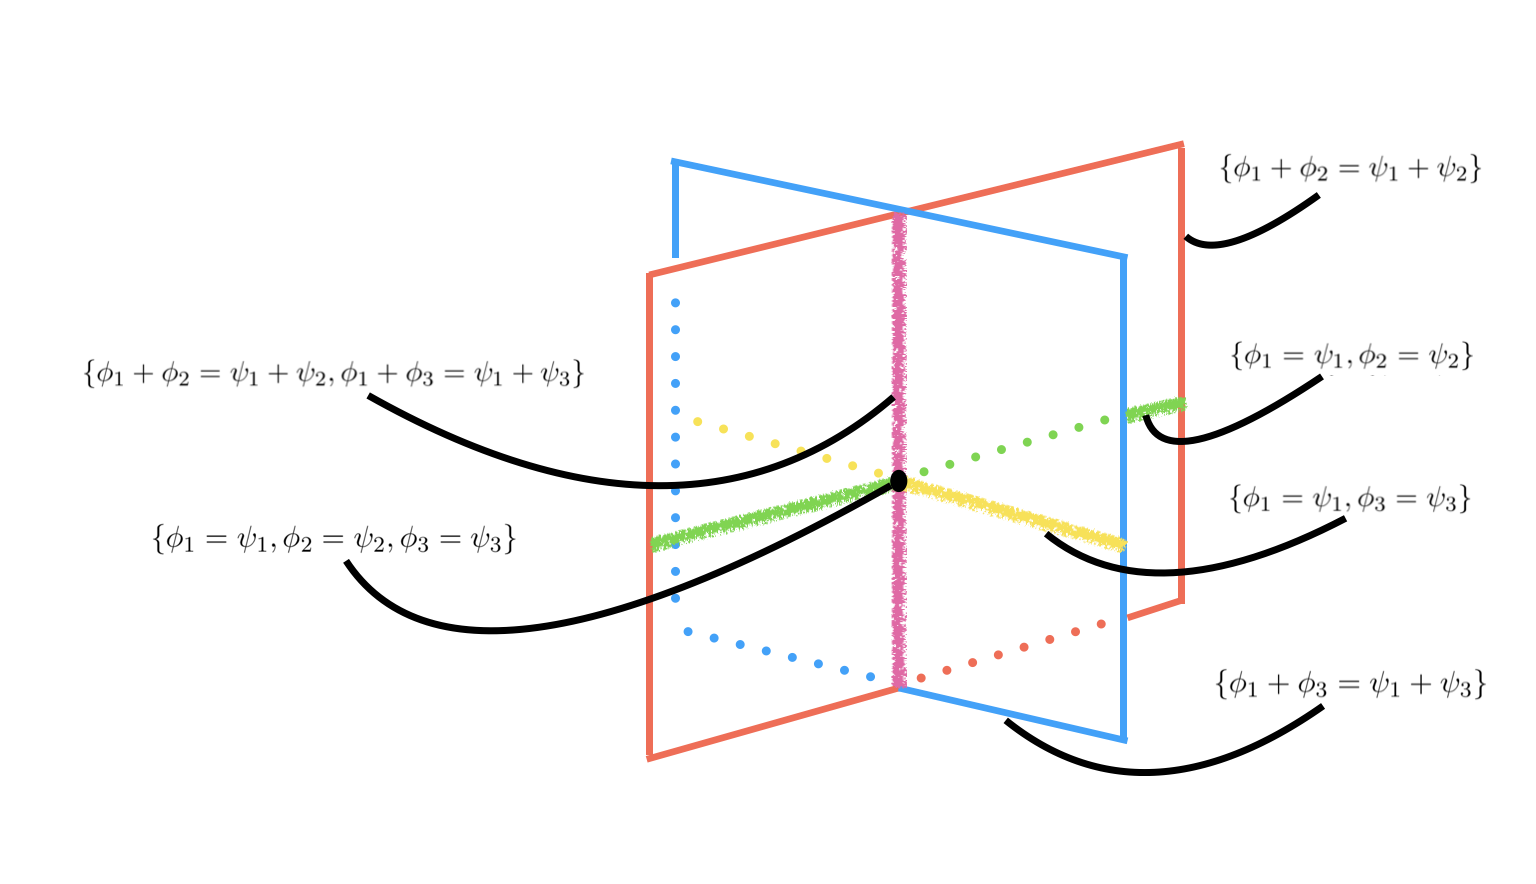
\includegraphics[scale = 0.5]{overlap.png}
 \caption{Four subtypes of cells,  simplexes of $(\phi,\psi)$ satisfying different constraints.}
  \label{fig:1}
\end{figure}
\hfill\\
In figure 1, there are four subtypes, the rectangle with magenta boundary is a simplex $A_{\pi_1} = \{(\phi,\psi) : \phi_1 + \phi_2 = \psi_1 + \psi_2\}$, the rectangle with blue boundary is a simplex $A_{\pi_2} = \{(\phi,\psi) : \phi_1 + \phi_3 = \psi_1 + \psi_3\}$. The green line refers to $A_{\pi_3} = \{(\phi,\psi) : \phi_1 = \psi_1, \phi_2 = \psi_2\}$, the yellow line refers to $A_{\pi_4} = \{(\phi,\psi) : \phi_1 = \psi_1, \phi_3 = \psi_3\}$, the purple line refers to $A_{\pi_5} = \{(\phi,\psi) : \phi_1 + \phi_2 = \psi_1 + \psi_2, \phi_1 + \phi_3 = \psi_1 + \psi_3\}$, which is the intersection of $A_{\pi_1}$ and $A_{\pi_2}$, and finally the black dot which is the intersection of those three lines refers to the simplex with finest partitions, $\phi_i = \psi_i, \forall i = 1,..,4$. We lack posterior inference for $(\phi,\psi)$ along the purple line except the black dot. While on the green line, yellow line and black dot, we have consistent posterior inference(theorem 2). To explain why some space lacking posterior inference and define such space, we define a special subset $A_\pi^*$ of simplex $A_\pi$. $A_\pi^* = A_\pi\setminus \underset{\tilde{\pi} \text{ is not coarser than } \pi }\cup A_{\tilde{\pi}}$, $A_\pi^*$ is obtained by removing all intersection with other $A_{\tilde{\pi}}$(excluding those $A_{\tilde{\pi}}$ that is superset of $A_\pi$) from $A_\pi$. Since we removed those intersection parts. It is intuitive that $A_\pi^*$ will be disjoint subsets of $\Omega$.\\
\begin{prop}
if $\pi_1 \neq \pi_2$, then $A_{\pi_1}^*\cap A_{\pi_2}^* = \emptyset$
\end{prop}
\hfill\\
Let $Q = \Omega\setminus \underset{\pi\in \Pi}\cup A_\pi^*$, first thing to check is whether $Q$ exists.\\
\begin{prop}
Let $K$ be number of subtypes. When $K >  3, Q_2 \neq \emptyset$, when $K \leq 3, Q_2 = \emptyset$
\end{prop}
\hfill\\
When number of subtypes bigger than three, we lack posterior inference on $Q$. To see that we can rewrite $A_\pi^*$ as $A_\pi^* = A_\pi\setminus \underset{\tilde{\pi} \text{ is not coarser than } \pi }\cup (A_{\tilde{\pi}}\cap A_\pi)$, $\tilde{\pi}$ is not coarser than $\pi$, which is equivalently to say $\pi$ is not refinement of $\tilde{\pi}$. By lemma 1, $A_{\tilde{\pi}}\cap A_\pi$ is a lower dimensional subset of $A_\pi$. So $A_\pi \setminus A_\pi^*$ is a lower dimensional subset of $A_\pi$. For posterior on $Q$, it degenerates to integral on a lower dimensional subset of the simplex associating with densities, which will vanish\\
\begin{prop}
When $K >  3$, $p(Q | z^1, z^2) = 0$
\end{prop}
\hfill\\
But for $(\phi, \psi)\in \Omega\setminus Q$, we have consistent posterior inference. Assuming $\alpha_i = 1, \forall i$ in (2) and $\beta_b = \Sigma_{i\in b} \alpha_i$ in (3), plug in (4) then we have simplified 
\begin{align}
p(A_\pi| z^1, z^2) = \frac{1}{c'}\sum_{\pi' \in \text{RF}(\pi)}\prod_{b\in \pi'}\frac{ \Gamma(\beta_b + t_b^1 + t_b^2)}{\Gamma(\beta_b + t_b^1)\Gamma(\beta_b + t_b^2)}
\end{align}
$c' = c/\frac{\Gamma(n + 1)\Gamma(n+1)\Gamma(K)}{\Gamma(2n + K)}$ And we have theorem 2.\\
\begin{theorem} Let $n = min(n_1, n_2)$ be the smaller number of cells of two conditions and $n_1 = O(n_2)$, when parameter $(\phi, \psi)\in \Omega\setminus Q $ we have 
\begin{eqnarray*}
    p(A_{\pi} | z^1, z^2) \xrightarrow[n\rightarrow\infty]{\text{a.s.}}\left\{
                \begin{array}{ll}
                 1 \quad \text{if }(\phi,\psi) \in A_\pi\\
                 0 \quad \text{otherwise}\\             
                \end{array}
              \right.
\end{eqnarray*}
\end{theorem}
\hfill\\
Things become more complicate when $(\phi, \psi)$ falling into $Q$, we know $p(Q | z^1, z^2) = 0$, but $p(A_\pi | z^1, z^2)$ may not vanish even the sample size is sufficiently large. Recall $N(\pi)$ represents number of blocks $b$ in $\pi$. Let $S = \{\pi,  (\phi, \psi) \in A_\pi\}$, which is the collection of partitions whose associated simplexes covering $(\phi,\psi)$. Let $N^* = \underset{\pi\in S}\max$ $N(\pi)$, which is the max number of blocks of partitions from $S$. Let $S^* = \{\pi,  (\phi, \psi) \in A_\pi \text{ and } N(\pi) = N^*\}$, which is the collection of partitions that covering $(\phi, \psi)$ with number of blocks equal to the max number $N^*$. For example, when $K = 7$, For a $(\phi, \psi)\in A_{\pi_1} \cap A_{\pi_2} \cap A_{\pi_3}$, $\pi_1 = \{\{1,2,3\}, \{4,5,6,7\}\}, \pi_2 = \{\{1,6,7\}, \{2,4\},\{3,5\}\}, \pi_3 = \{\{1,2,3,4,5,6\}\}$, and also $(\phi, \psi)$ does not belong to any other simplex $A_\pi$. Then $S = \{\pi_1, \pi_2, \pi_3\}$, $N^* = 3$, $S^* = \{\pi_2\}.$ Denote components from right hand side of (5): $\frac{1}{c'}\underset{b\in \pi}\prod\frac{ \Gamma(\beta_b + t_b^1 + t_b^2)}{\Gamma(\beta_b + t_b^1)\Gamma(\beta_b + t_b^2)} = w(z^1,z^2,\pi).$  We have theorem 3.\\
\begin{theorem} Following the setting in theorem 2, when parameter $(\phi, \psi)\in Q$,  and we have 
\begin{eqnarray*}
    w(z^1,z^2,\pi) \xrightarrow[n\rightarrow\infty]{\text{a.s.}}\left\{
                \begin{array}{ll}
                 m(\pi) \quad  \pi \in S^* \\
                 0 \quad \text{otherwise}\\             
                \end{array}
              \right.
\end{eqnarray*}
and $\underset{\pi\in S^*}\sum m(\pi) = 1, m(\pi) > 0$\\
\end{theorem}\hfill\\
proofs are in the appendix.\\
Still using above example, in limiting case, we have $p(A_{\pi_3} | z^1, z^2) = 1$, $p(A_{\pi_2} | z^1, z^2) = 1$ and $p(A_{\pi_1}| z^1, z^2) = 0$. When the DE pattern is $B_{\pi_1}$ for some genes. Since our underestimation of $p(A_{\pi_1}| z^1, z^2) = 0$, we will falsely classify those genes as differential distributed.



\section{Data analysis workflow} 
\subsection{simulated data}\hfill\\
Here's an example using the probabilities $\phi$ and $\psi$ from Figure 2;
\begin{figure}[h!]
  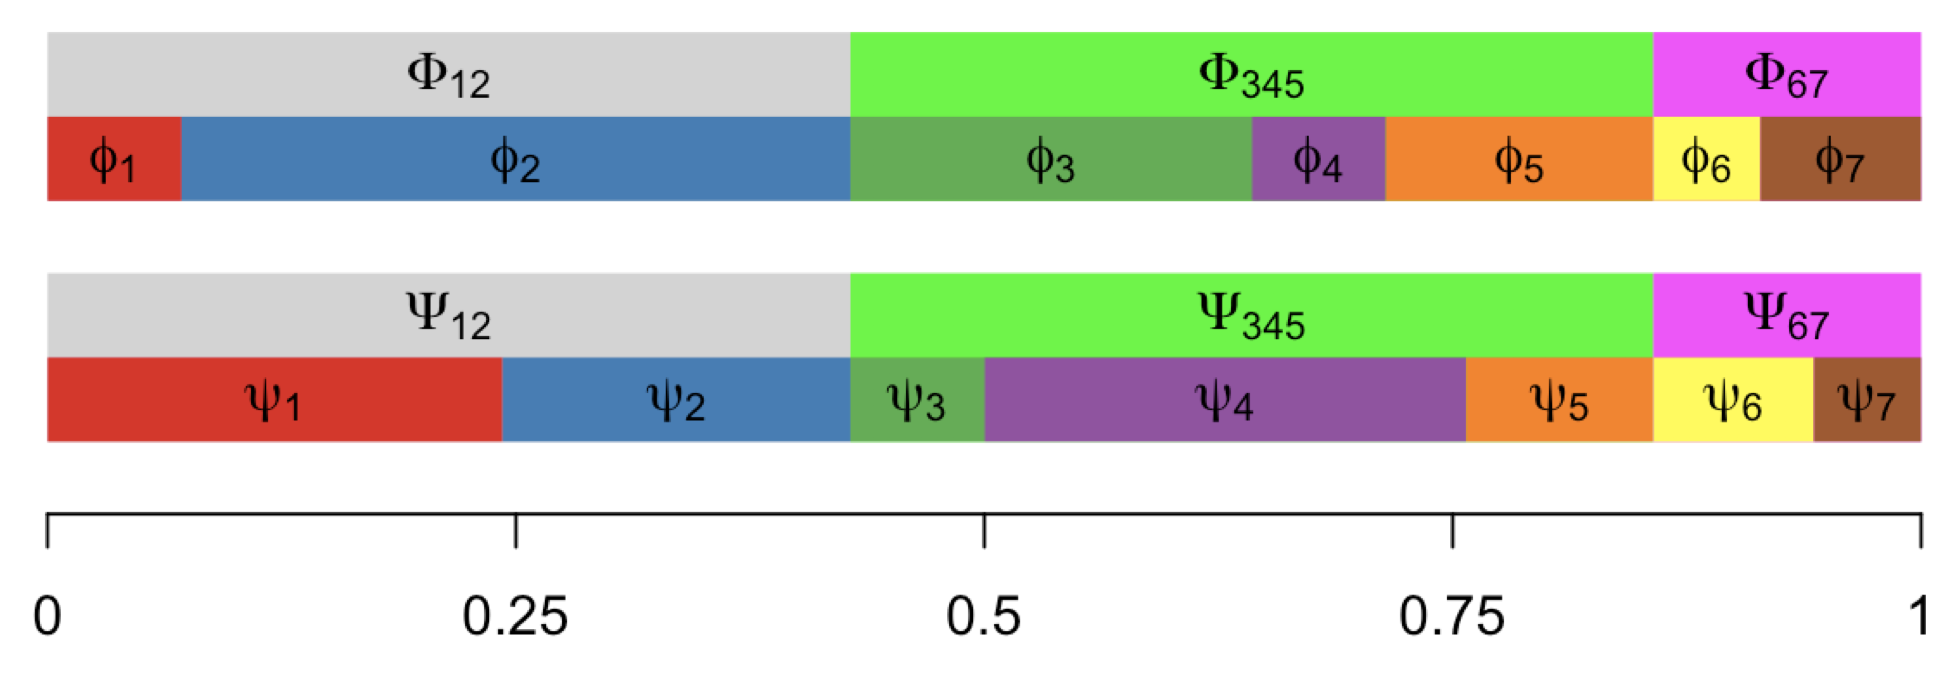
\includegraphics[height = 4cm, width=\linewidth]{prop.png}
  \caption{proportions of subtypes change in different conditions.}
  \label{fig:2}
\end{figure}
We simulate data by splatter\cite{ref:Zappia} with $n_1=n_2=200$, and 7 subtypes among two conditions with constraints of proportions: $\phi_1 + \phi_2 = \psi_1 + \psi_2$, $\phi_3 + \phi_4 +\phi_5 = \psi_3 + \psi_4 + \psi_5$ and $\phi_6 + \phi_7 = \psi_6 + \psi_7$\\
We view the differences among subtypes by projecting transcripts profiles of cells into its first two principal components(figure 3)
\begin{figure}[h!]
  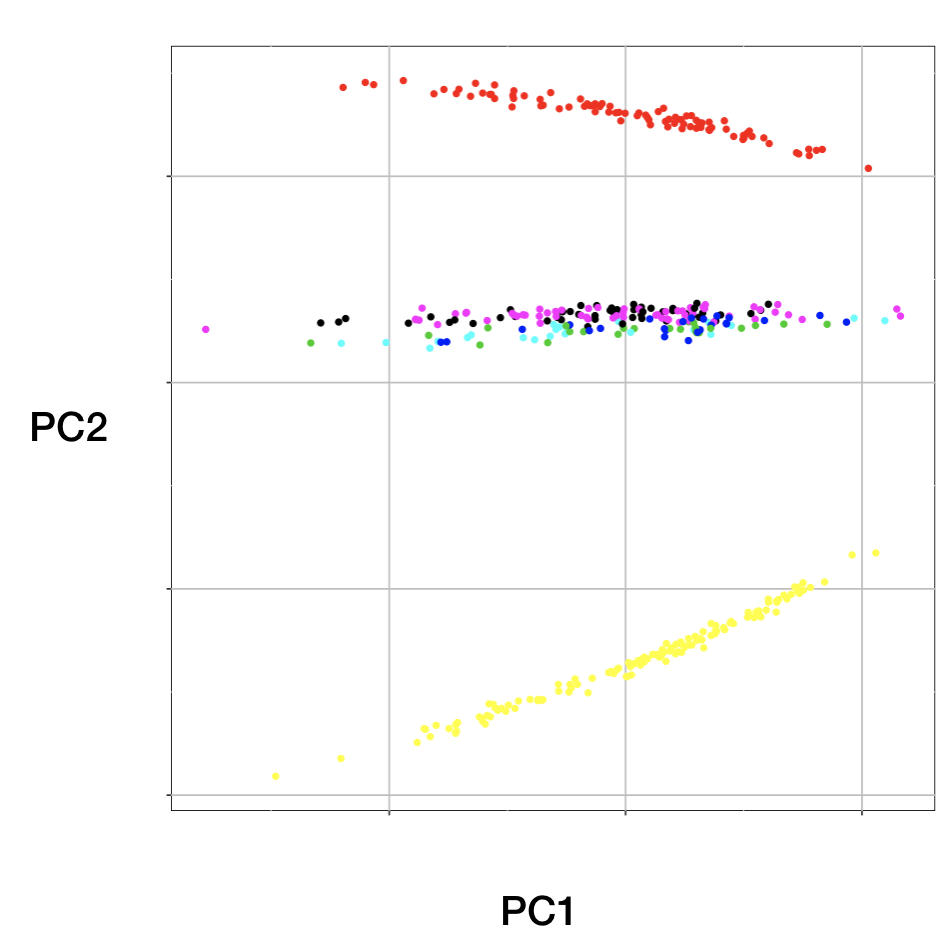
\includegraphics[height=8cm, width=8cm]{pca.png}
  \caption{first two principal components of transcripts, which demonstrates the difference between subtypes. Even if we projected transcripts of cells into two dimensional space, we observe subtypes are separated.}
  \label{fig:4}
\end{figure}


\subsection{The scDDboost modeling framework}\hfill\\
1.\textit{Normalization.} Raw transcripts are normalized by SCnorm\cite{ref:Rhonda} adjusted for technical sources of variation including amplification bias and sequencing depth\\
2.\textit{Distance calculation.} We use the clustering method in section 2 to calculate distances between cells.\\
3.\textit{Clustering} Given a number of clusters, do K-medoids based on distance matrix calculated in step 2.\\   
4.\textit{DE analysis.} After clustering of cells, we obtain posterior inference on differential expression pattern among subtypes via EBSeq\cite{ref:Leng}\\
5.\textit{Posterior of proportion.} We obtain posterior inference on proportion change via the double dirichlet prior in section 2. \\
6.\textit{Posterior of DD.} Combine results from step 4 and 5 to compute posterior probabilities of genes being differential distributed\\
We determine the number of clusters by searching a range of candidates (from 1 to 9 based on our empirical experience). Given a number of cluster, we compute the posterior probabilities of genes being differential distributed by step 4 - 6. We visualize the change between posterior probabilities under number of clusters $i$ and $i + 1$($i$ from 1 to 8). It typically remains stable when number of cluster is above a number smaller than 9 (figure 4)\\
In the splatter simulation setting, there are 7 groups and 10\% genes each group are DE genes. There are in total 9067 DD genes and 8306 ED genes.\\
Below are numbers of DD or DE genes identified by four methods with target FDR at 5 \%. \\
\begin{tabular}{ |p{3cm}|p{3cm}|p{3cm}|p{3cm}|p{3cm}|}
\hline
 & scDDboost & scDD & MAST & DESeq2\\
\hline
\hline
DD or DE genes & 6073 & 3038 & 2468 & 2076\\
\hline
True positive & 4774 & 2724 & 2442 & 2073\\
\hline
false positive & 1299 & 314 & 26 & 3\\
\hline
\end{tabular}\\
\captionof{table}{number of true positive and false positive genes identified by four methods. Target FDR at 5\%}
scDDboost identified most true DD genes, the reason is that some DE genes in the simulation have small log fold change and make the regular two sample test difficult to detect the change, especially when method did not consider mixture of subtypes, which could further make the change insignificant. scDDboost could correctly identify the subtypes of cells and thus are more sensitive to the mean expression change among subtypes. We also compare roc curves of scDDboost, scDD, MAST and DESeq2. (figure 5)
\begin{figure}[h]
\vspace{-\parskip}
\minipage{0.5\textwidth}
  \includegraphics[width=\textwidth]{sim_67.png}
\endminipage\hfill
\minipage{0.5\textwidth}
  \includegraphics[width=\textwidth]{sim_78.png}
  \endminipage
\caption{comparison of posterior probabilities of being DD among different number of subtypes, when we underestimate the number of subtypes, the difference is huge, see PDD between 6 subtypes and 7 subtypes. When we overestimate the number of subtypes, though inflating PDD (intercept is greater than 0 in the right panel) but the variation of difference is small, we observe a linear relation between PDD of 7 subtypes and 8 subtypes}
\end{figure}
\begin{figure}[h]
  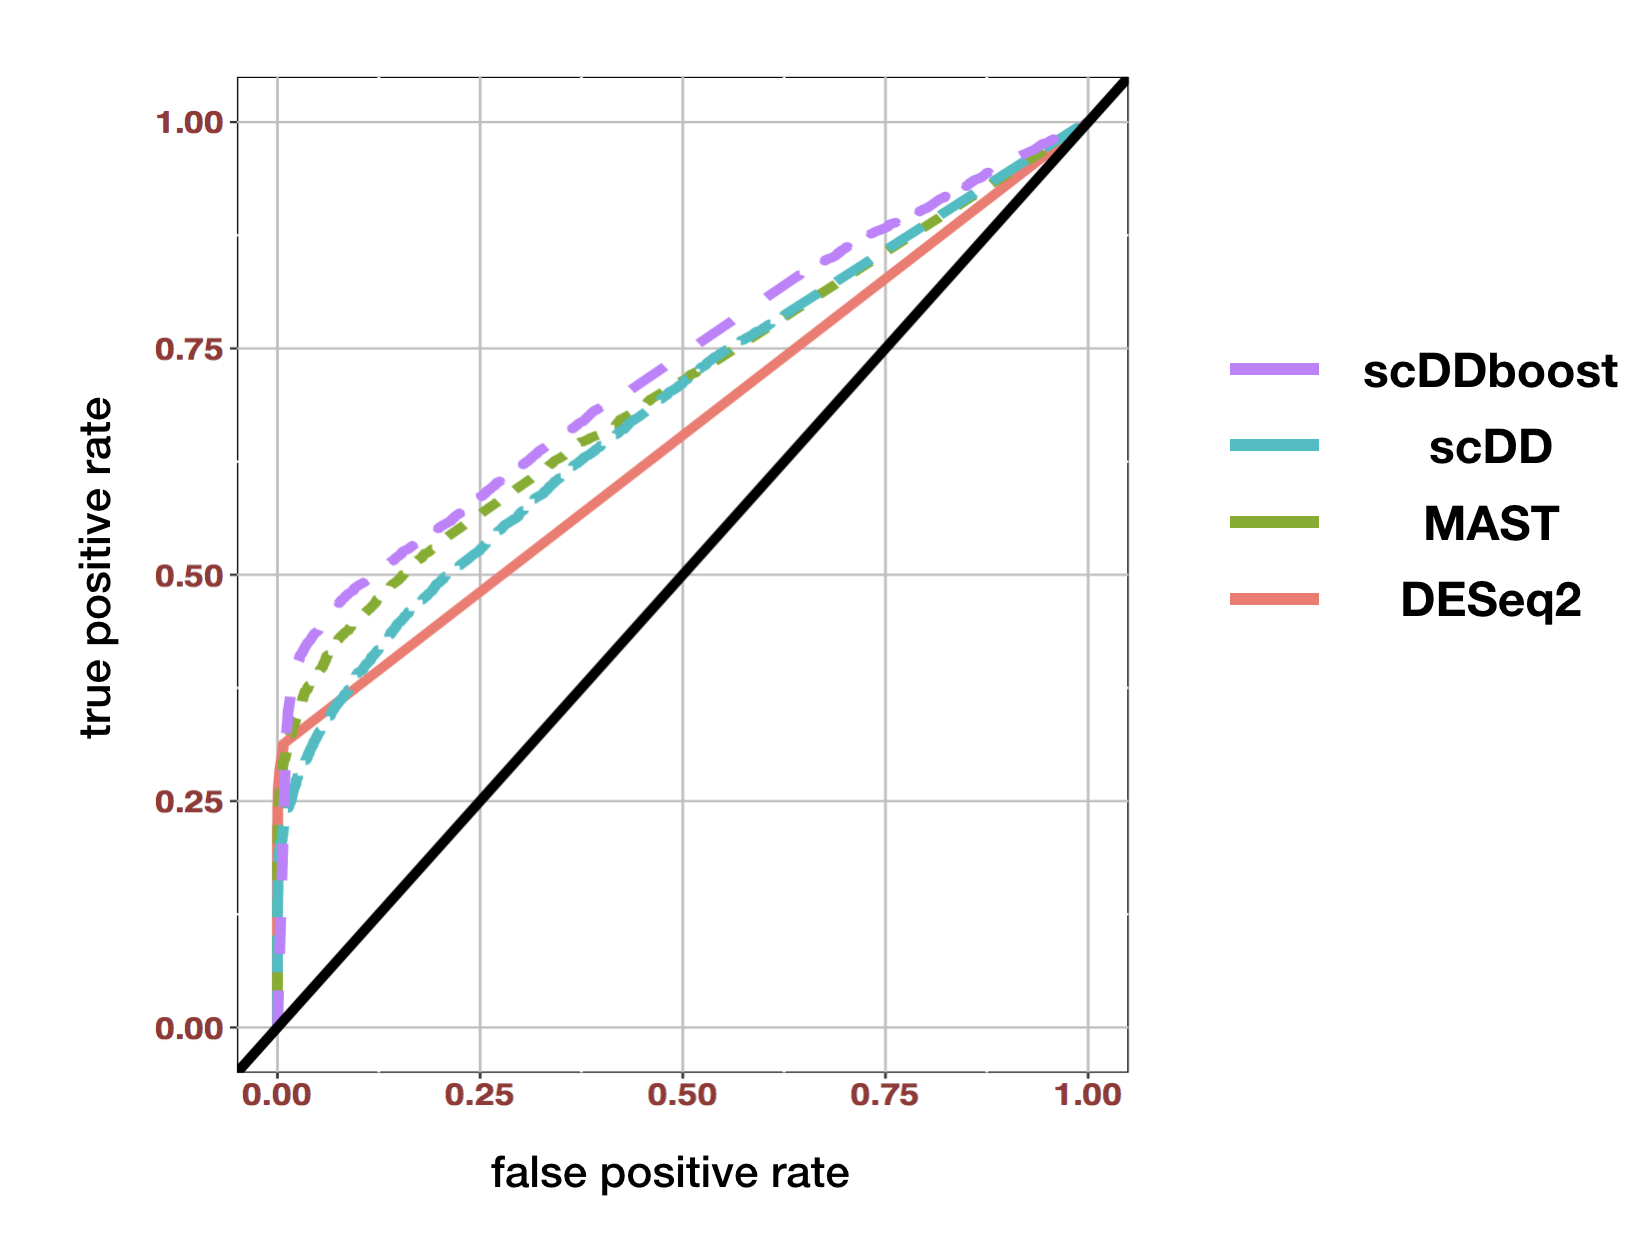
\includegraphics[height = 6cm]{roc.png}
  \caption{Roc curve of scDDboost, scDD, MAST and DESeq2, scDDboost has largest area under the roc curve. Roc curves of Mast and scDD are similar. For those roc curve there is bigger difference at low level of false positive rate, as scDDboost identified twice many true DD genes as other methods.}
  \label{fig:5}
\end{figure}
scDDboost may work poorly, when $(\phi, \psi)\in Q$, like we have discussed in section 2.5, we may underestimate the posterior probability of true proportion change pattern, which reduce the posterior probabilities of true negative and enlarge false positive rate.\\
Since we are modeling gene transcript within each subtype as negative binomial distributed and we only test one parameter(mean) change among subtypes. In some situation, it could be insufficient for modeling the variability within subtype, which leads to another situation that the power of scDDboost could be limited. Even though there is no mean expression change among subtypes but the distribution among subtypes changed, EBSeq would fail to detect the discrepancies between subtypes, thus reduce power of detecting DD genes.\\
\section{Examples}
We use ten datasets from conquer\cite{ref:Cq} to test performance of our method on real data. We compare our results with scDD\cite{ref:scDD}, MAST\cite{ref:MAST} and DESeq2\cite{ref:Des}\\
\begin{center}
\begin{tabular}{ |p{3cm}|p{6cm}|p{2cm}|p{2cm}|p{1cm}|}
\hline
 Data set & Compared cell subsets & Number of cells per condition & Organism & Ref\\
 \hline
 \hline
 GSE45719 & 16-cell stage blastomere vs Mid blastocyst cell (92-94h post- fertilization) & 50, 60 & mouse & \cite{Deng193}\\
 \hline
 GSE45719null &  16-cell stage blastomere & 50 & mouse &  \cite{Deng193}\\
 \hline
 GSE48968-GPL13112 & BMDC (1h LPS stimulation) vs BMDC(4h LPS stimulation) & 96, 95 & mouse & \cite{Shalek}\\
 \hline
 GSE48968-GPL13112null & BMDC (1h LPS stimulation) & 96 & mouse & \cite{Shalek}\\
 \hline
 GSE60749-GPL13112 & v6.5 mouse embryonic stem cells, culture conditions: 2i+LIF vs v6.5 mouse embryonic stem cells, culture conditions: serum+LIF & 90, 94 & mouse & \cite{Kumar}\\
 \hline
 GSE60749-GPL13112null & v6.5 mouse embryonic stem cells, culture conditions: 2i+LIF & 90 & mouse & \cite{Kumar}\\
 \hline
 GSE74596 & NKT0 vs NKT17 & 45,44 & mouse & \cite{Engel}\\
 \hline
 GSE74596null & NKT0 & 45 & mouse & \cite{Engel}\\
 \hline
 
 EMTAB2805 & G1 vs G2M & 96,96 & mouse & \cite{EMTAB}\\
 \hline
 EMTAB2805null & G1 & 96 & mouse & \cite{EMTAB}\\
 \hline
 GSE63818-GPL16791 & Primordial Germ Cells, develop- mental stage: 7 week gestation vs Somatic Cells, developmental stage: 7 week gestation & 39,26 & mouse & \cite{Guo}\\
 \hline
 GSE71585-GPL13112 & Chrna2 tdTpositive vs Cux2 tdTpositive & 84, 124 & mouse & \cite{Tasic}\\
 \hline
GSE71585-GPL13112null & Chrna2 tdTpositive & 84 & mouse & \cite{Tasic}\\
\hline
GSE75748 & NPC vs DEC & 64, 87 & human & \cite{chu}\\
\hline
GSE75748 & NPC & 64 & human & \cite{chu}\\
\hline
GSE75748 & DEC vs EC & 70, 64 & human & \cite{chu}\\
\hline
GSE75748 & DEC & 70 & human & \cite{chu}\\
\hline
GSE64016null & H1 exp1 vs H1 exp2 & 64, 87 & human & \cite{oscope}\\
\hline
\end{tabular}
\captionof{table}{single cell transcripts profiles used for differential expression or distribution method evaluation}
\end{center}
\hfill\\
We have table of numbers of differentially expressed genes of each dataset by MAST and DESeq2, and numbers of differentially distributed genes of each dataset by scDDboost and scDD.\\
\\
\begin{center}
\begin{tabular}{ |p{2cm}|p{2cm}|p{2cm}|p{2cm}|p{2cm}|p{2cm}|p{2cm}|}
\hline
Data set & scDDboost & scDDboost-sc3 & scDD & MAST & DESeq2 & total number of genes\\
\hline
\hline
GSE45719 & 5758 & 4228 & 6416 &5652 & 11202 & 45686\\
\hline
GSE48969-GPL13112 & 11691 & 9819 & 2080 & 3396 & 9542 & 45686\\
\hline
GSE60749-GPL13112 & 19215 & 19168 &  18074 & 13674 & 23178 & 45686\\
\hline
GSE74596 & 1942 & 1353 & 1099 & 540 & 3796 & 45686\\
\hline
EMTAB 2805 & 5295 & 3748 & 2202 & 1088 & 5391 & 45686\\
\hline
GSE63818-GPL16791 & 3948 & 3480 & 1365 & 873 & 8934 & 45686\\
\hline
GSE71585- GPL13112 & 2902 & 1460 & 1622 & 2572 & 7378 & 24057 \\
\hline
NPC-DEC & 4377 & 3211 & 5982 & 6666 & 8439 & 19037\\
\hline
DEC-EC & 3402 & 3023 & 3818 & 5429 & 8127 & 19037\\
\hline
H1 exp1-H1 exp2 &  0 & 0 & 1300 & 2077 & 2841 & 16579\\
\hline
\end{tabular}
\captionof{table}{number of genes detected as significantly DE or DD}
\end{center}
We found that bulk method DESeq2 tends to have the most number of DE genes. But among single cell methods we found that scDDboost usually had the most number of DD genes we indeed increase the power of DD genes detection. Further we observed quite a few genes uniquely identified by scDDboost are likely to have different distribution across conditions. For example, figure 6, we use heatmap to demonstrate the log expression profiles among DEC and EC. \\
\begin{figure}[h]
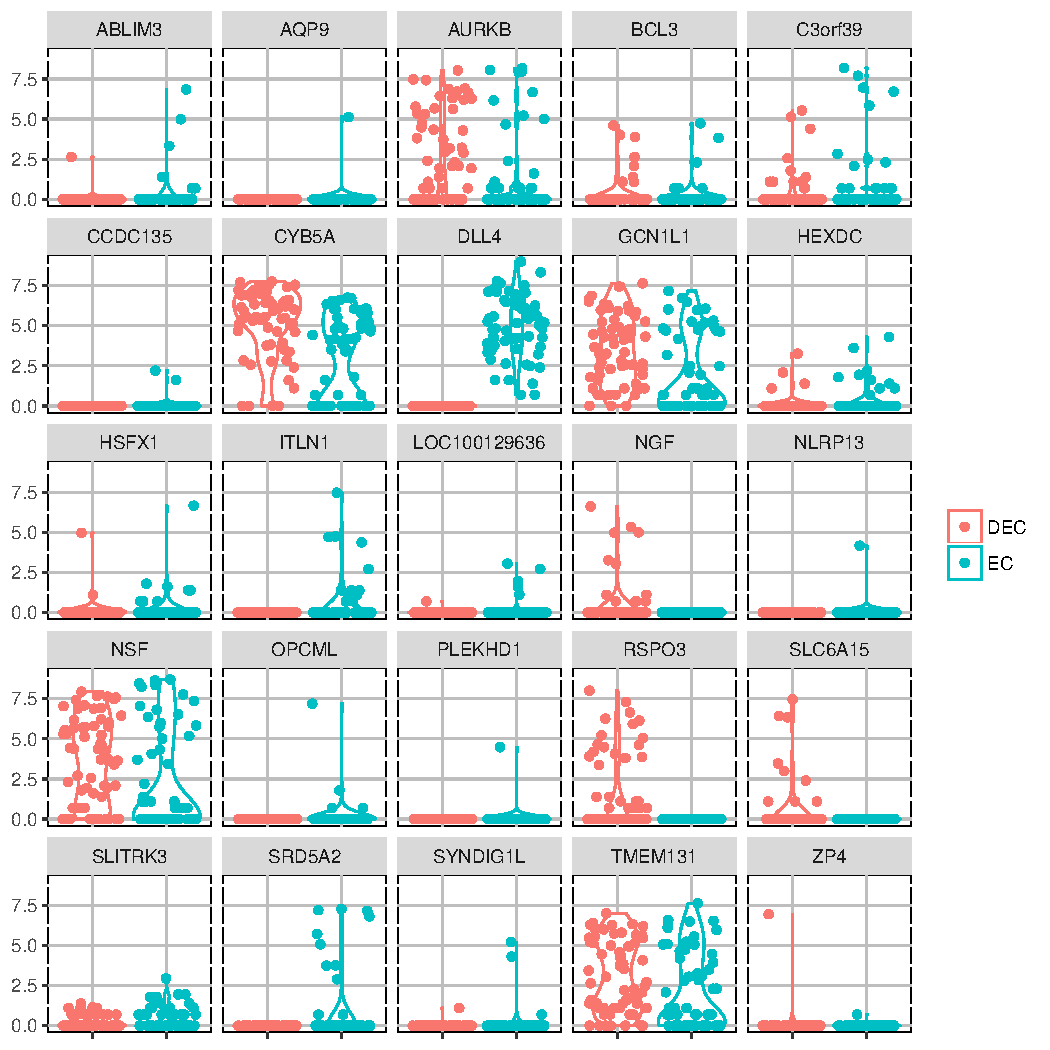
\includegraphics[width = \textwidth]{density.pdf}
 \caption{ Densities of log transformed transcripts 25 DD genes uniquely identified by scDDboost, for data GSE75748, DEC vs. EC, We observe some of the genes are different distributed across conditions. *** may need other plot to further investigate those genes that are appear to be DE but identified as DD***}
  \label{fig:6}
\end{figure}
Although bulk methods seems to be the most powerful one, we found it also has a higher false discovery rate comparing to single cell methods. We validate false discovery rate on ten null datasets from table 1. For each null dataset, we randomly split the cells from one condition into two equal sized subsets and do DE analysis between those subsets. Since those two subsets of cells actually came from same condition, there should not be any differential distributed genes, any positive call would be a false positive. We repeat the random split and testing for five times on each null data set. We evaluate the type I error control for the methods returning nominal p-values, by recording the fraction of genes(with a valid p-value) that are assigned a nomial p-value below 0.05 (figure 5).\\
\begin{figure}[h]
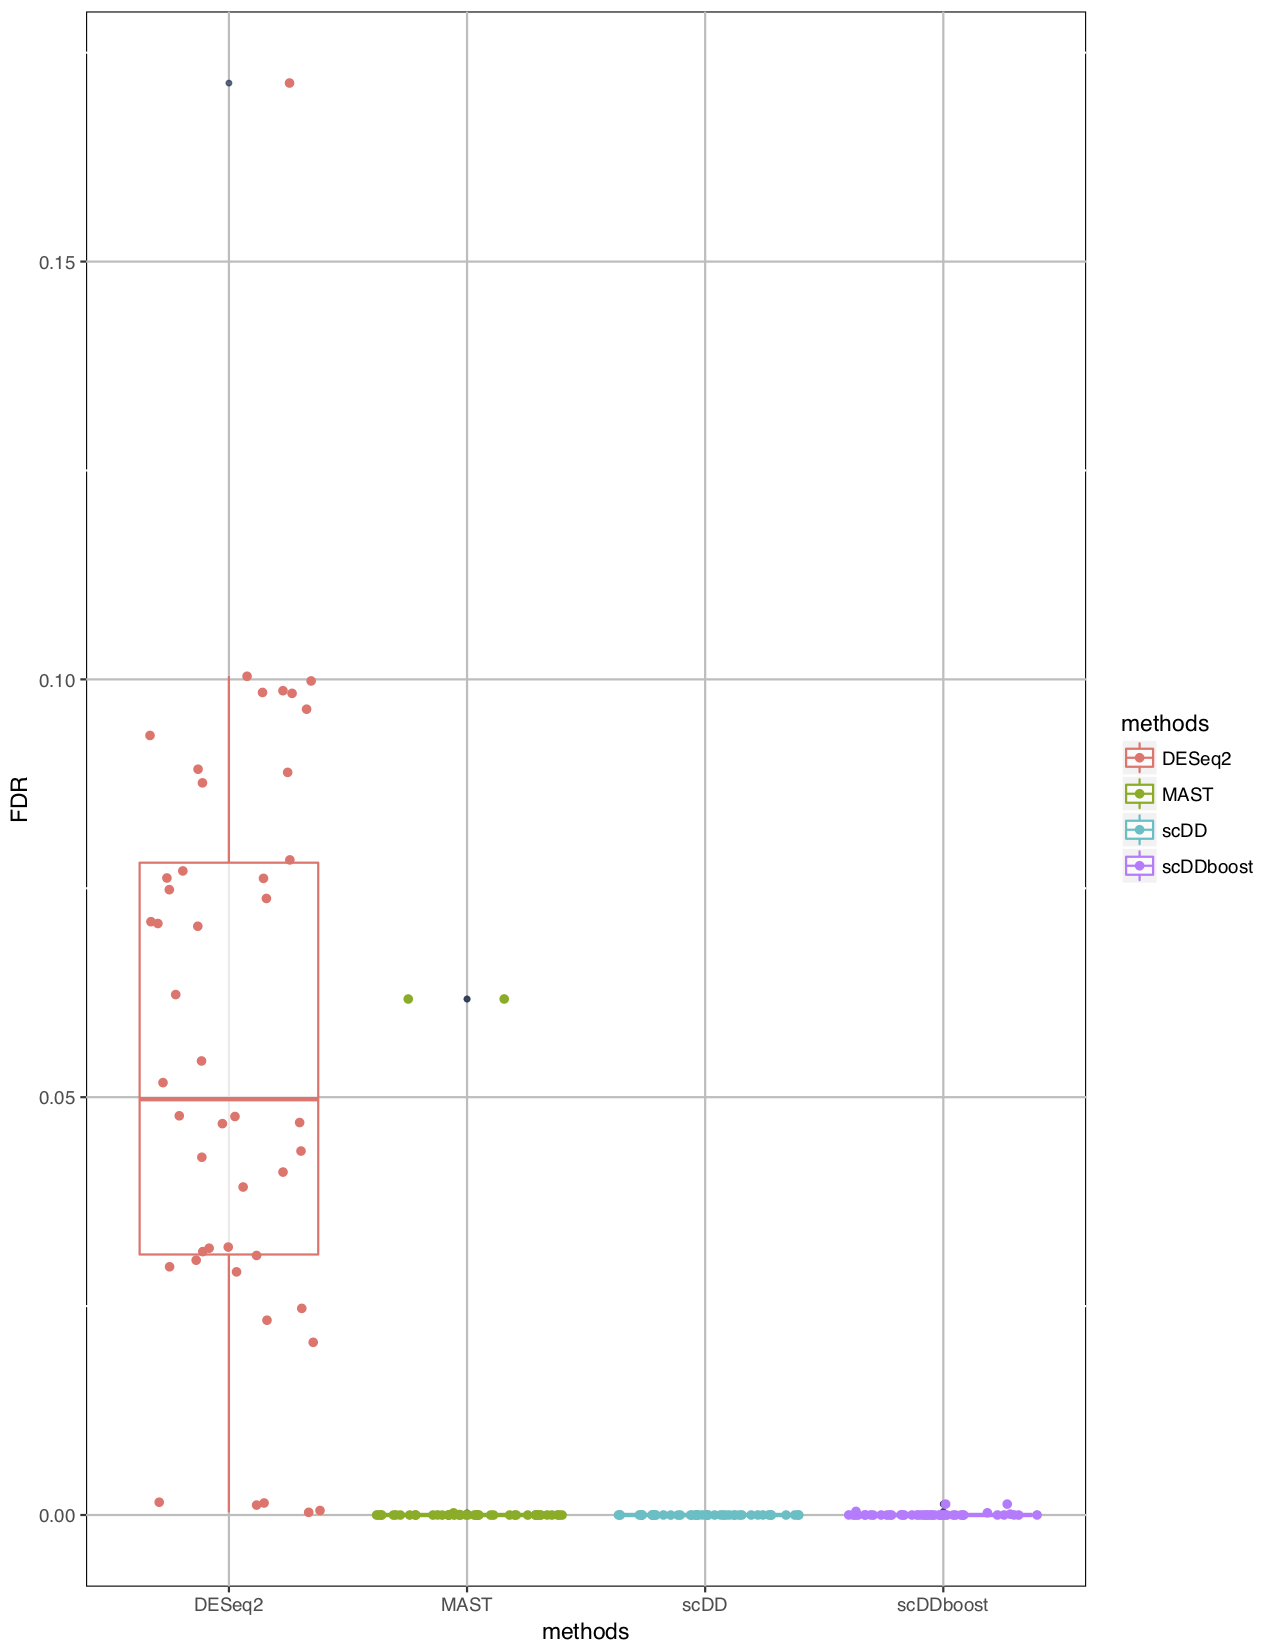
\includegraphics[width = 8cm]{FDR.png}
 \caption{FDR of scDDboost, scDD, MAST and DESeq2 on null dataset from table 1, DESeq2 usually identify a lot but may lose the control of type I error. While other single cell methods could control FDR. ***This procedure for testing FDR,  we randomly split a population into two samples, so it is highly likely proportion of subtypes remain same among these two samples, scDDboost always give small PDD and almost make no false positive call. This is kind different from really examining the FDR of scDDboost, where we have different proportions across conditions, but we do not want false call on those genes without mean expression change even there is proportion change. In this case, it actually reduce to the FDR of EBSeq whether we make correct posterior inference on DE pattern. The test of proportion is only done once, so scDDboost could still control FDR*** }
  \label{fig:7}
\end{figure}
scDDboost could control FDR since we assume cells are sampled from population composed of different subtypes. Cells from one subtype are equal likely to be assigned to either one of the two subsets. Consequently, proportions of subtypes remain unchanged among the two subsets.\\
D3E\cite{ref:d3e} is a distributional method that can identify bursting parameters of transcripts. Rate of promoter activation, rate of promoter inactivation and the rate of transcription when the promoter is in the active state are estimated by D3E.  We investigate DD genes identified by scDDboost and their change of those three parameters on dataset EMTAB2805\\
\begin{figure}[H]
\vspace{-\parskip}
\minipage{0.33\textwidth}
  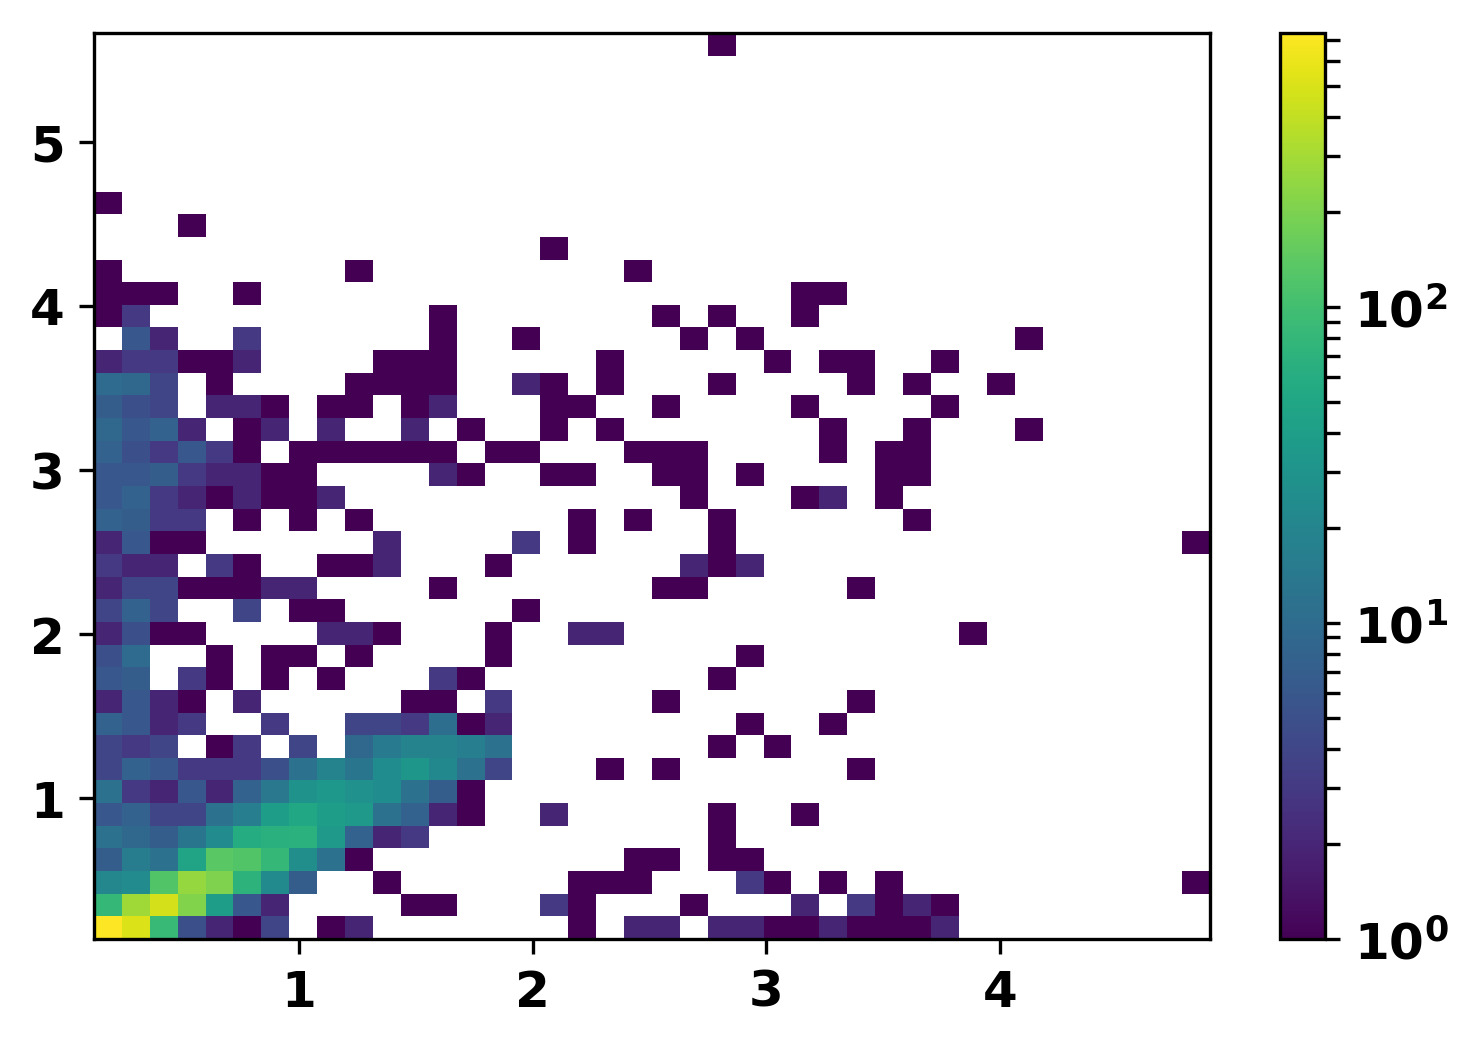
\includegraphics[clip,width=\textwidth]{act.png}
  \captionsetup{labelformat=empty}
  \caption{A}
\endminipage
\minipage{0.33\textwidth}
  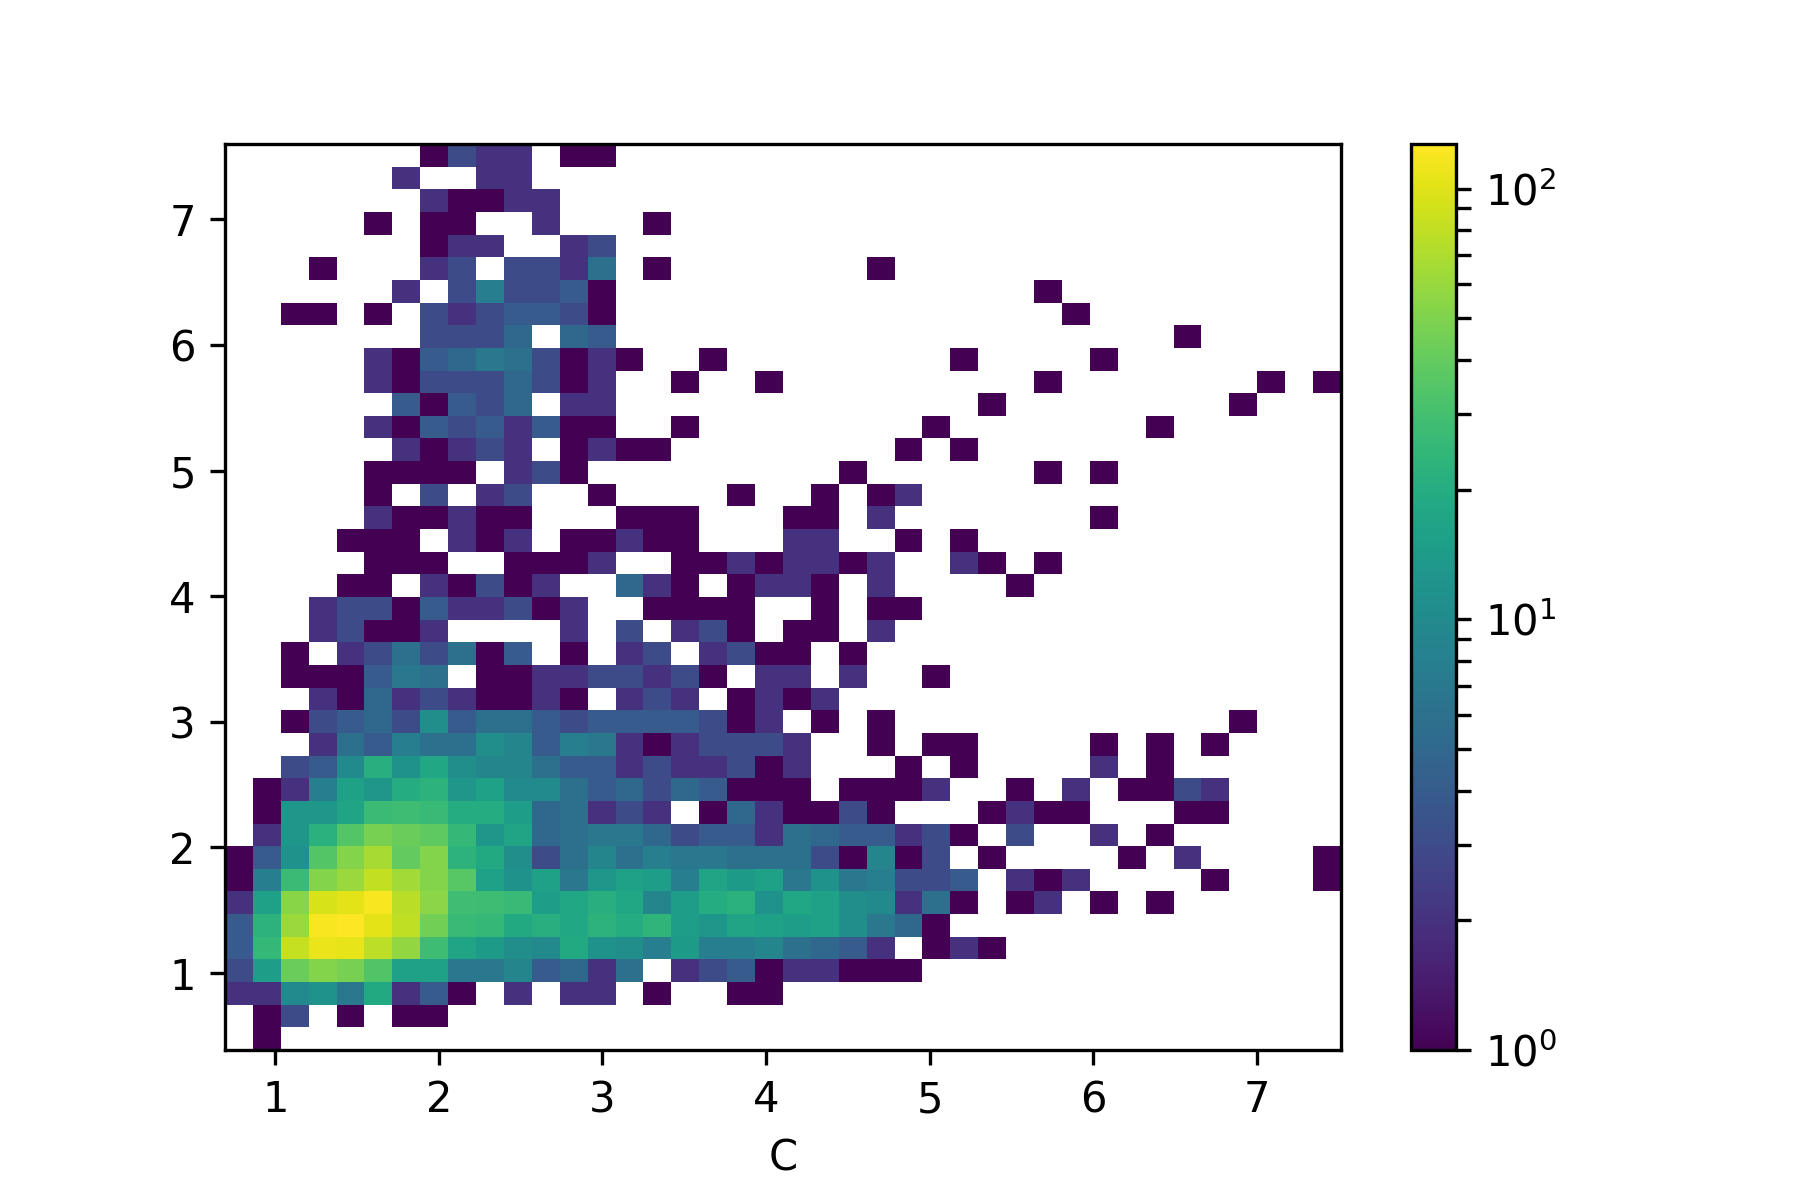
\includegraphics[clip,width=\textwidth]{in_act.png}
  \captionsetup{labelformat=empty}
  \caption{B}
  \endminipage
 \minipage{0.33\textwidth}
  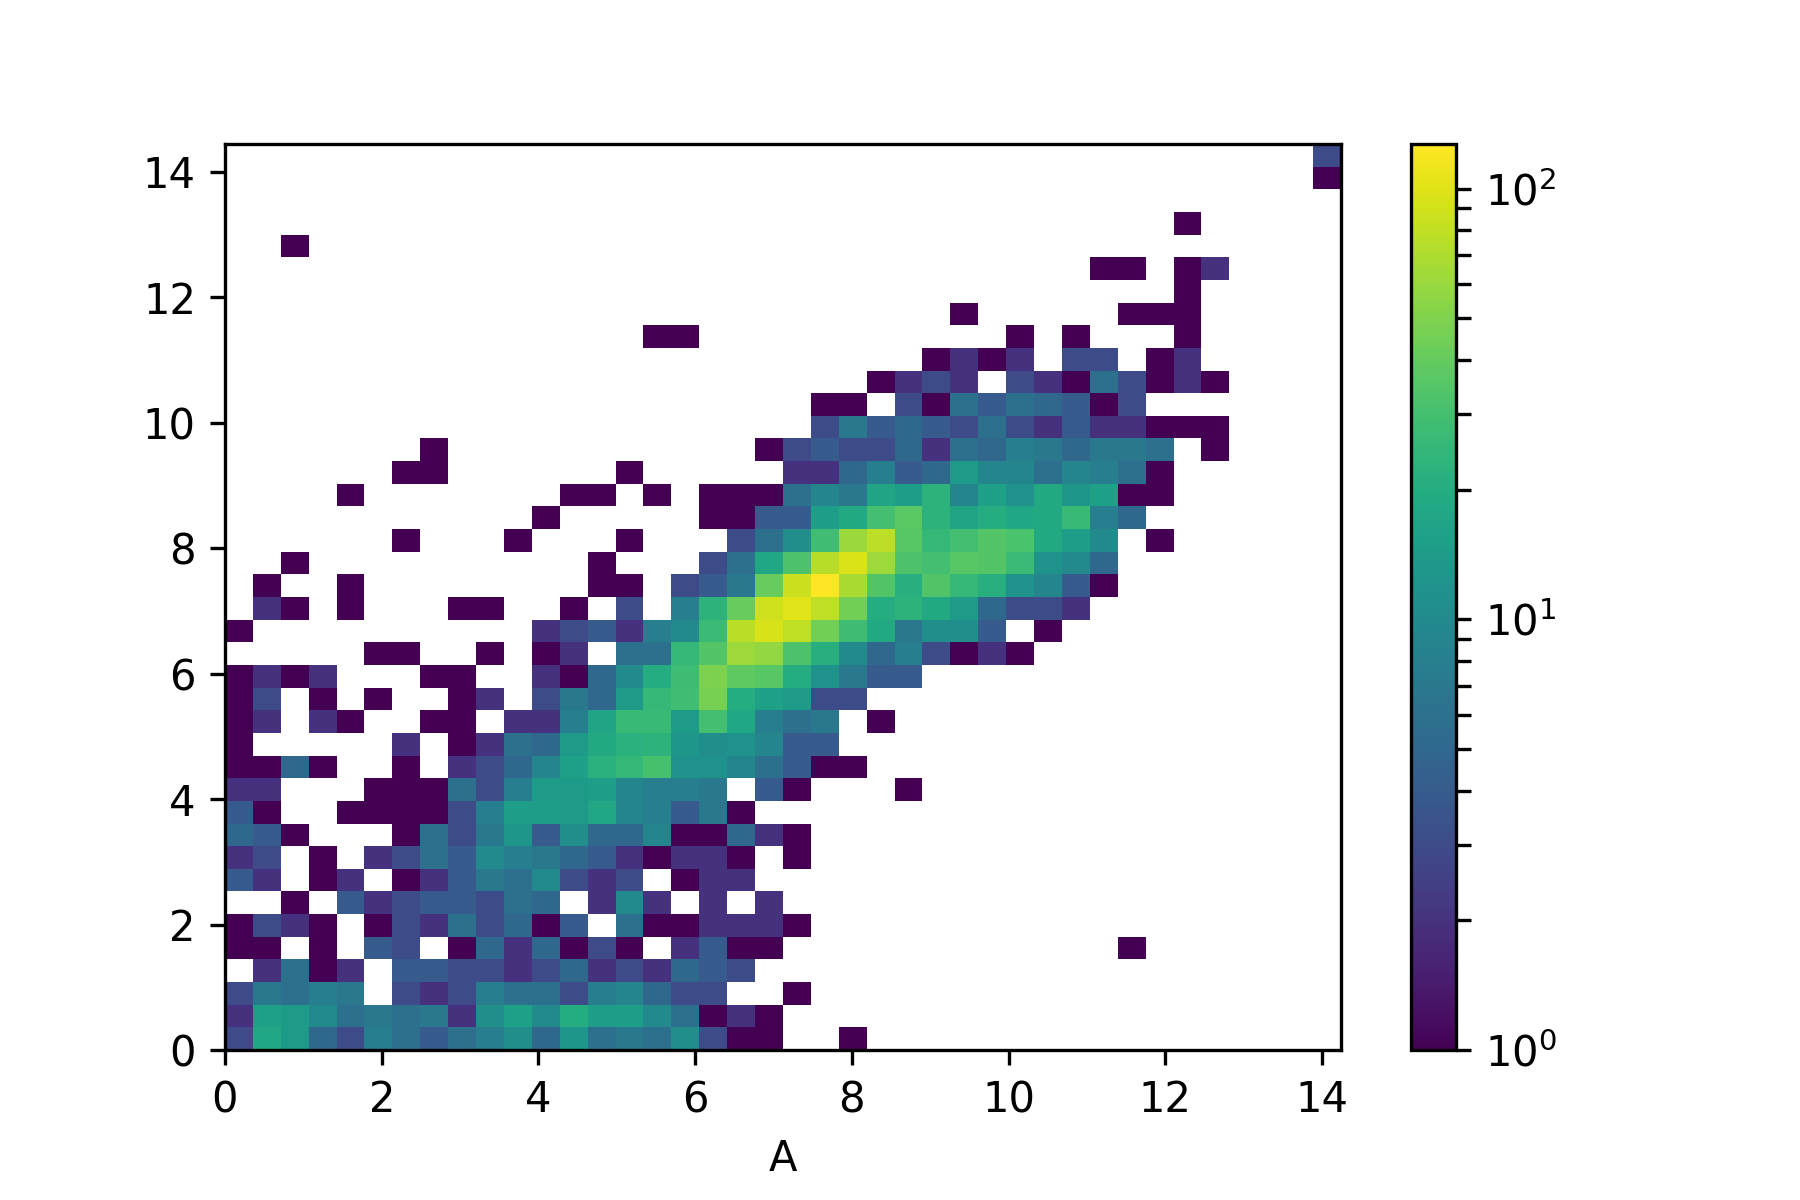
\includegraphics[clip,width=\textwidth]{t_rate.png}
  \captionsetup{labelformat=empty}
  \caption{C}
  \endminipage
\captionof{figure}{2D histogram for bursting parameters of DD genes identified by scDDboost from dataset EMTAB2805 estimated by D3E. Panel A : comparison of rate of promoter activation between two conditions, similarly, panel B : rate of promoter inactivation and panel C : rate of transcription when the promoter is in the active state. We observe that difference between transcription rate is smaller compare to difference between the activation and inactivation rate. ***other methods also observe similar phenomena, this is not unique to scDDboost, main reason is that estimation from D3E tends to give larger difference in activation and inactivation rate than transcription rate. We may argue the major factor to drive DD genes are activation and inactivation rate (proportions of different subtyps), so it make sense to consider mixture model like scDDboost.***}
\end{figure}
We observed that DD genes identified by scDDboost tends to have similar transcription rate when the promoter is active across condition, while there are lots of variabilities in the action and inactivation rate. These results reveal that DD genes identified by scDDboost are driven by the change of activation and inactivation rates. 

\section{Discussion}
Cluster cells is an unsupervised learning, we do not know the true underlying partition and different number of clusters will lead to large differences in posterior probabilities of genes being differentially distributed (figure 7). We propose a modified bootstrap to stabilize our inferences. Instead of resample the cells, we resample the distance matrices of cells by adding noises to original distance matrix. Denote the original distance matrix as $D = (d_{i,j})$, for each time we random sample a vector $e$ with length equal to number of cells and components are i.i.d. exponentially distributed. let $w$ be the standard deviation of $d_{i,j}$. We resample a new $\hat{D}$ by adding nosies: $\hat{d}_{i,j} = d_{i,j} + e_i * w + e_j *w$. For $\hat{D}$ we still have triangle inequality held as $\hat{d}_{i,j} + \hat{d}_{j,k} \geq \hat{d}_{i,k}$ , it is a valid distance matrix. For a fixed number of clusters, we average posterior probabilities over different distance matrices. And we select number of clusters $K$ that posterior probabilities do not vary too much under $K$ and $K+1$. From our empirical experience, it is typical $K$ will not be larger than 8.\\
\begin{figure}[H]
\minipage{0.5\textwidth}
  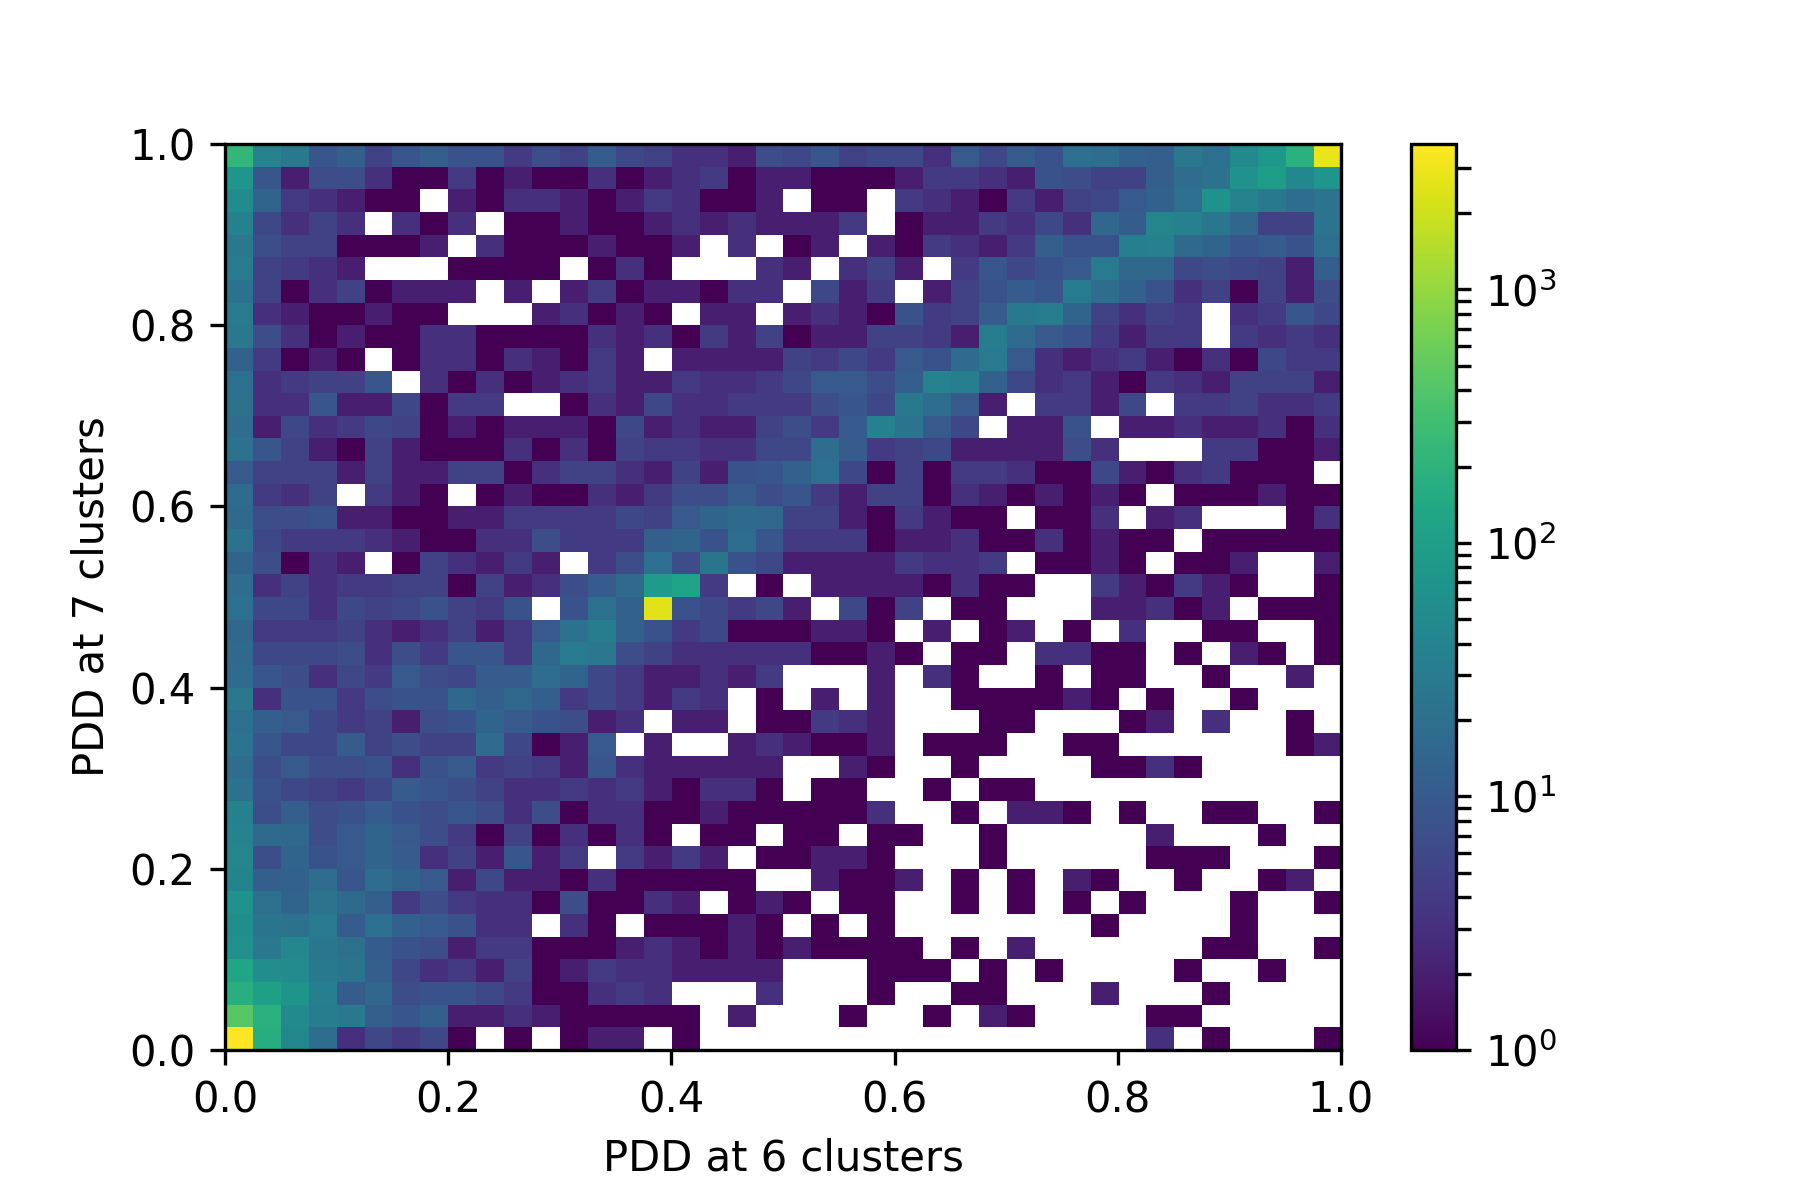
\includegraphics[height = 5cm, width=\linewidth]{DN_67.png}
\endminipage\hfill
\minipage{0.5\textwidth}
  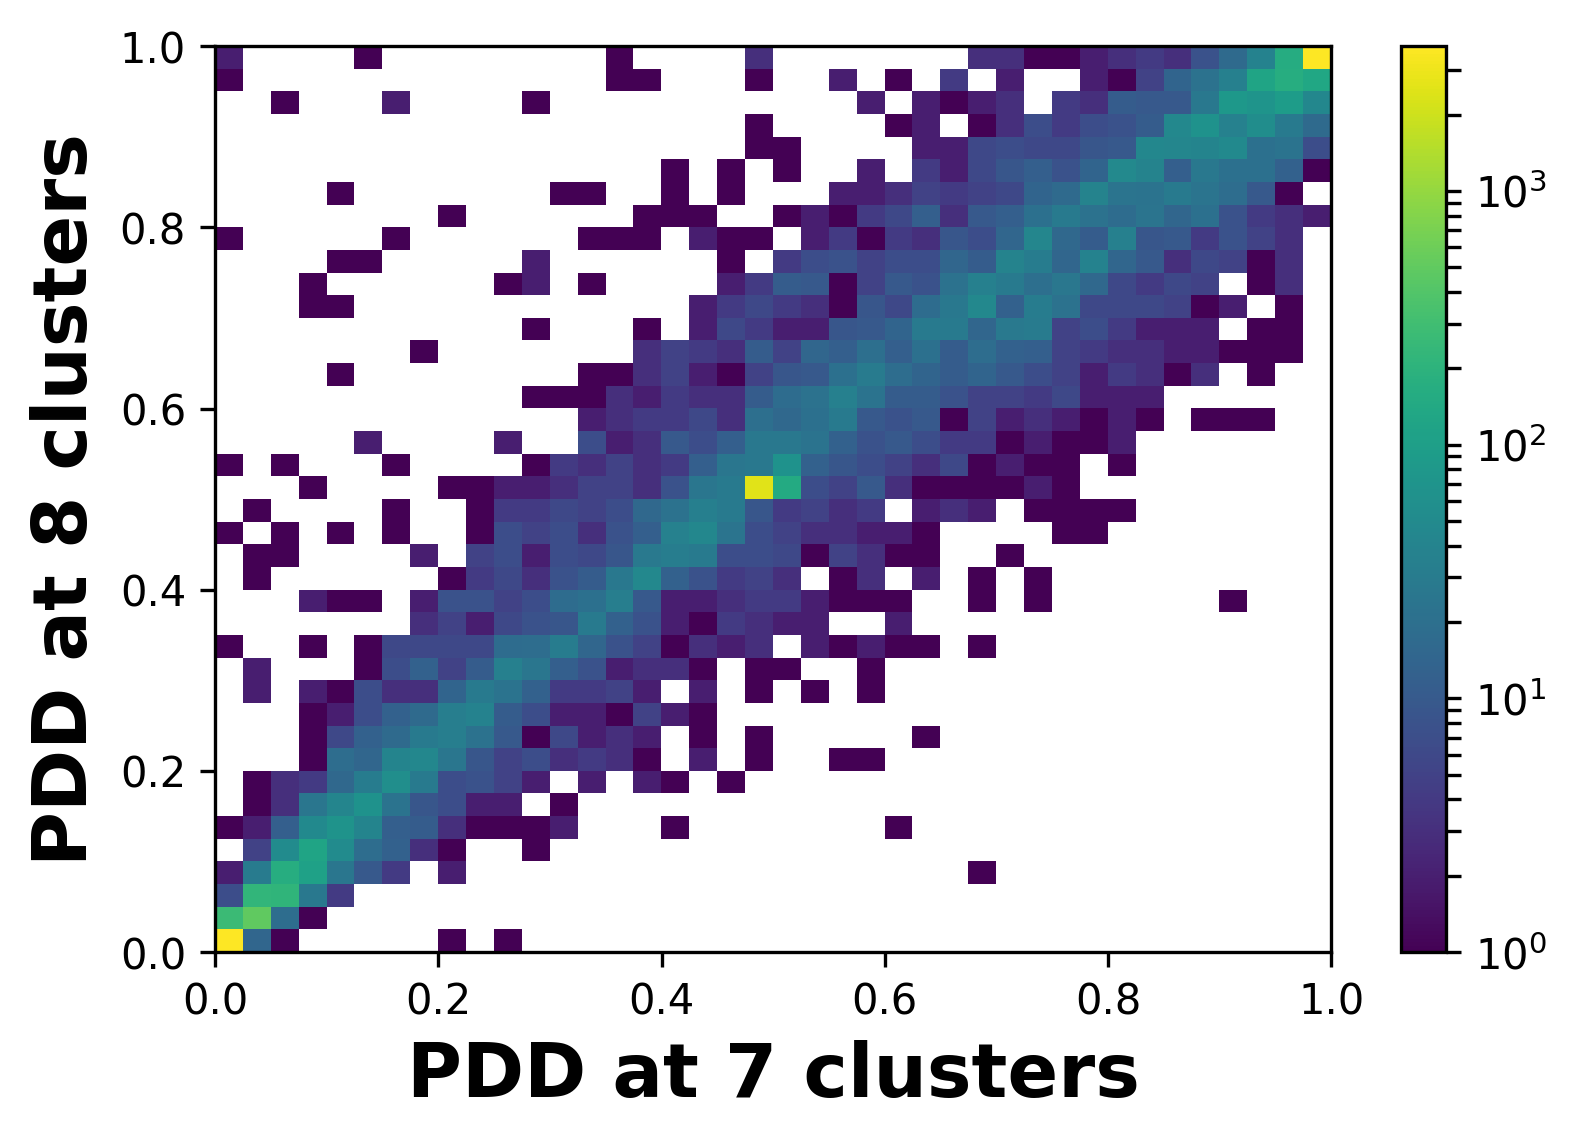
\includegraphics[height = 5cm, width=\linewidth]{DN_78.png}
\endminipage\hfill
\caption{selecting number of subtypes for data GSE75748, we observe posterior probabilities become stable at more than 6 subtypes. Since increasing number of subtypes tends to decrease sample size of each subtypes, make complicate constraints for equivalent distribution and inflate estimated PDD.  We select number of subtypes to be 7}
\end{figure}
\begin{figure}[H]
\minipage{0.5\textwidth}
  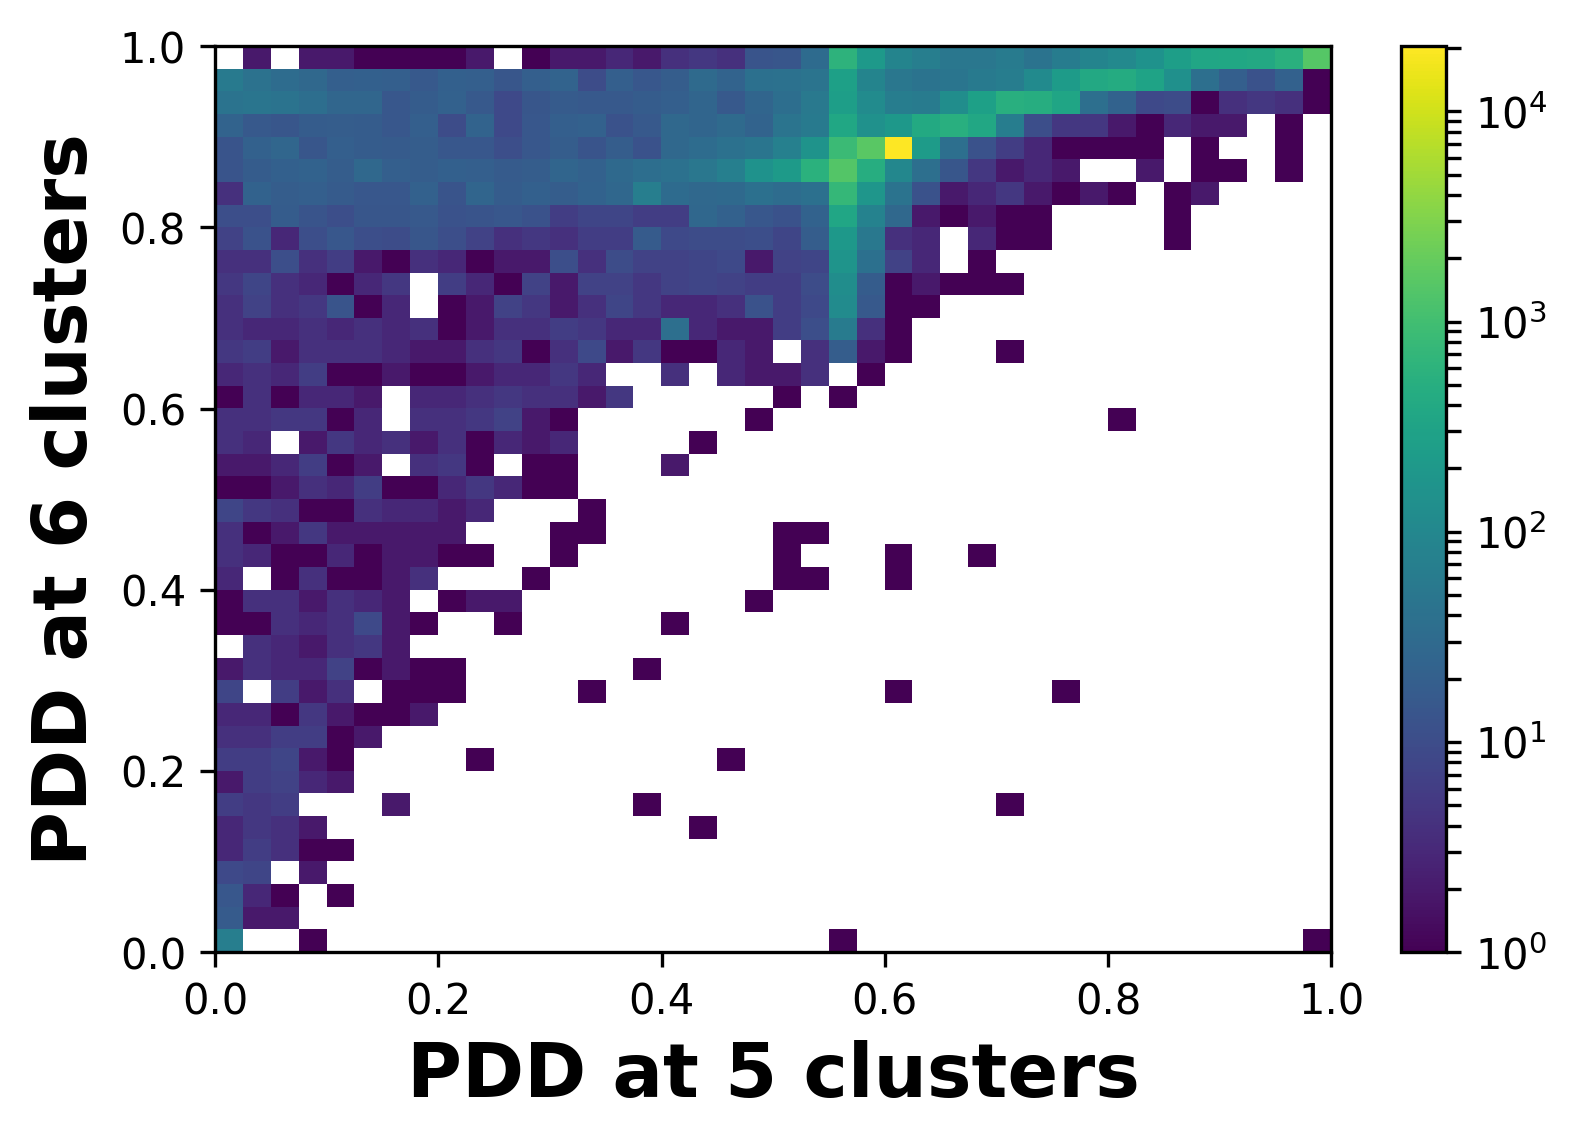
\includegraphics[height = 5cm, width=\linewidth]{G48_56.png}
\endminipage\hfill
\minipage{0.5\textwidth}
  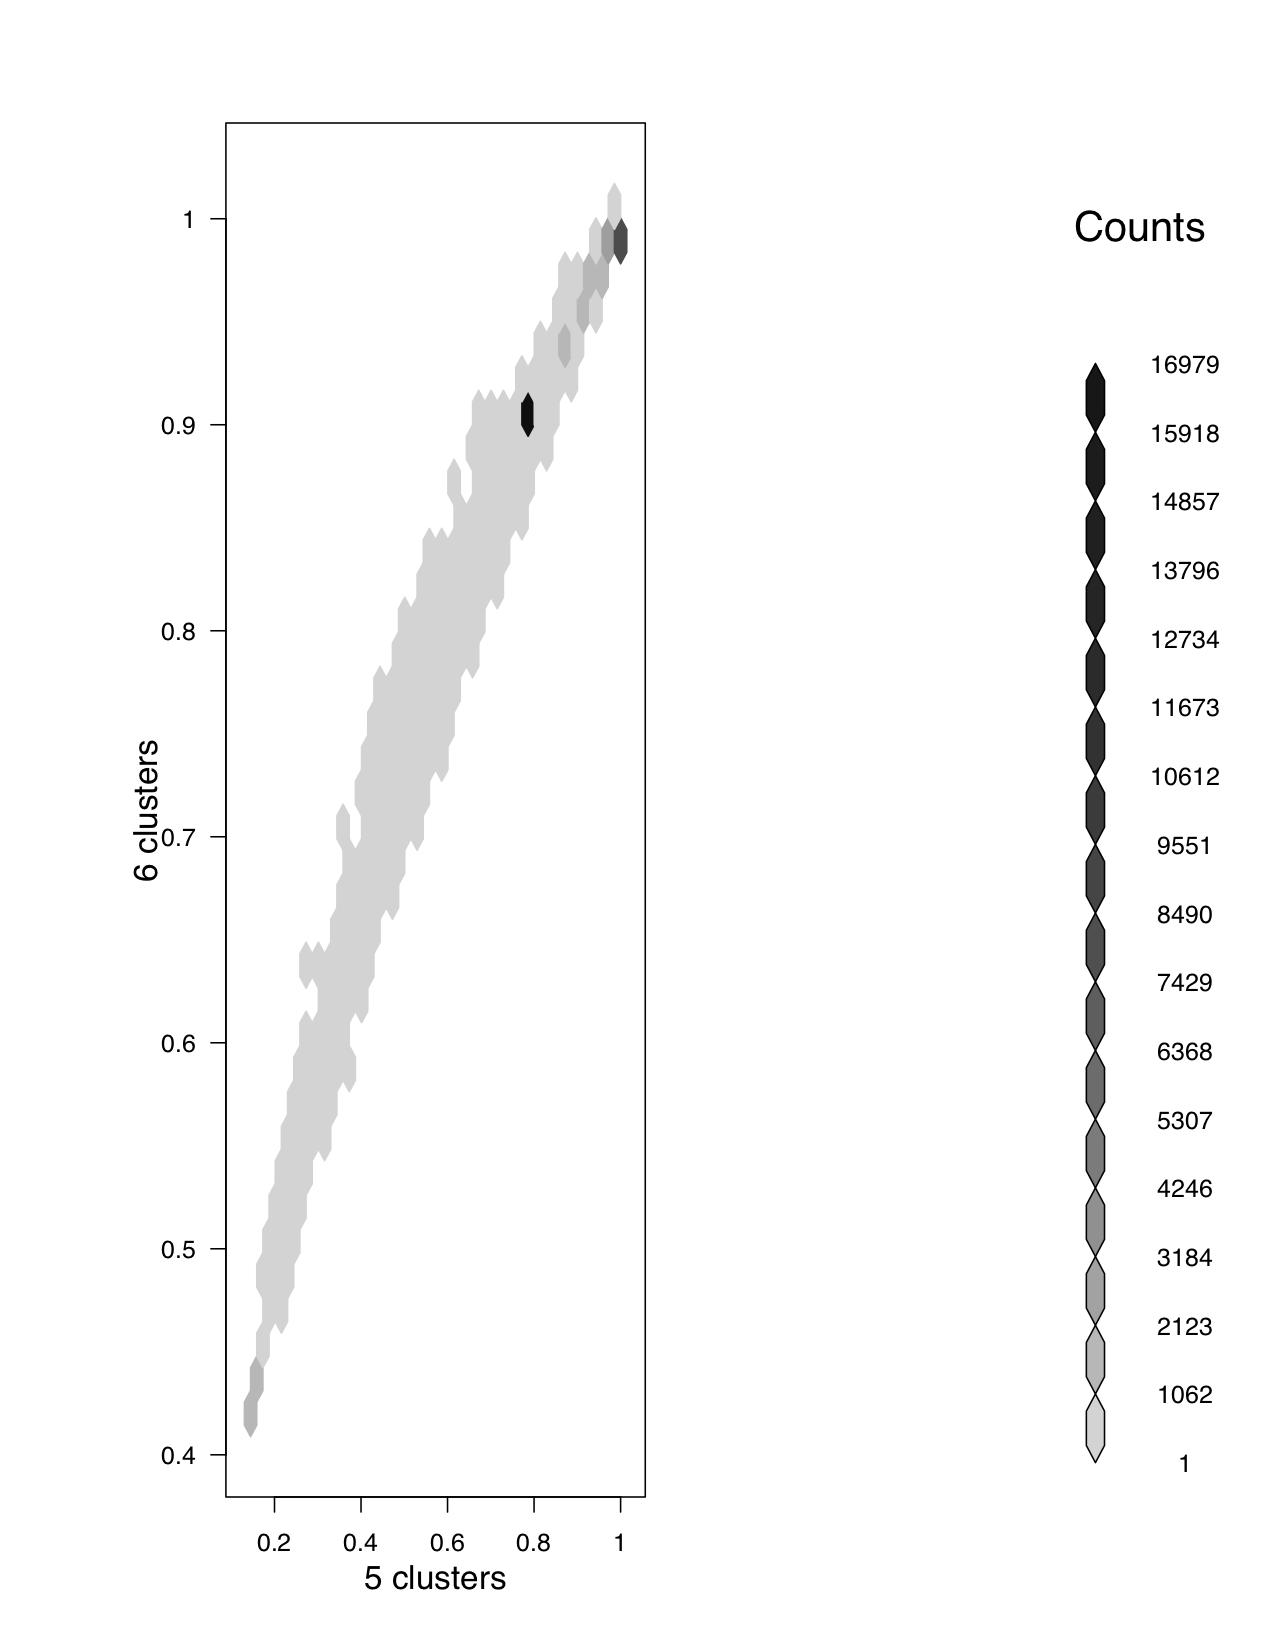
\includegraphics[height = 5cm, width=\linewidth]{G48_67.png}
\endminipage\hfill
\caption{selecting number of subtypes for data GSE48968, we observe posterior probabilities become stable at more than 5 subtypes}
\end{figure}


\newpage
\appendix
\section{}
\hfill\\
Proof of lemma 1
\begin{proof}
Let $V$ denote the orthogonal space of $\phi - \psi$, when $(\phi,\psi)\in A_{\pi_1} \cap A_{\pi_2}$, and $\text{dim}(A_{\pi_1} \cap A_{\pi_2}) = \text{dim}(\phi - \psi) + \text{dim}(\psi) = 2K - \text{dim}(V) - 1$. Also let $\pi_1 = \{b_1^1,...,b_s^1\}, \pi_2 = \{b_1^2,...,b_t^2\}$. The corresponding vectors are $v_1^1,...,v_s^1$ and $v_1^2,...,v_t^2$. We claim there must be a $b_i^1\in \pi$ whose corresponding $v_i^1$ is linear independent with $v_1^2,...,v_t^2$. If not, for every $v_i^1$ there exists $\alpha_1^i,...,\alpha_t^i$ such that 
\[
v_i^1 = \sum_{j = 1}^t \alpha_j^i v_j^2 \quad\quad\quad(*)
\]
If $b_j^2 \cap b_i^1 \neq \emptyset$, then multiply $v_j^2$ on both sides of (*), we obtain $v_i^1 * v_j^2 = \alpha_j^i (v_j^2)^2$, as $v_j^2$ are orthogonal vectors, and $v_i^1 * v_j^2 > 0$ implies $\alpha_j^i > 0$. Consider $x = f(b_j^2\setminus b_i^1)$, we have $x*v_i^1 = 0$ and we multiply $x$ on both sides of (*) to obtain $\alpha_j^i v_j^2*x = 0$, thus x must be zero vector and $b_j^2\setminus b_i^1= \emptyset$, which implies $b_j^2 \subset b_i^1$. That is to say when $b_j^2 \cap b_i^1 \neq \emptyset$, $b_j^2$ must be subset of $b_i^1$. So $b_i^1$ is union of some blocks in $\pi_2$. Which implies $\pi_2$ is refinement of $\pi_1$, contradiction.\\
Consequently there exists $b\in\pi_1$ with $v(b)$ linear independent with $v(b'), b'\in\pi_2$. $\text{dim}(V)$ is at least $N(\pi_2) + 1, \dim(A_{\pi_1} \cap A_{\pi_2}) < \text{dim}(A_{\pi_2})$
\end{proof}
\hfill\\
Proof of theorem 2 and theorem 3
\begin{proof}
Given the condition that $\alpha_k = 1, \forall k$ and $\beta_b = \sum_{k\in b} \alpha_k$, we can simplify $p(z^1, z^2 | A_\pi^*) = p(z^1 | t_{\pi^*}^1)p(z^2 | t_{\pi^*}^2)p(t_{\pi^*}^1, t_{\pi^*}^2 | A_{\pi}^*)$ and obtain $$p(z^1, z^2 | A_\pi^*) = \prod_{b\in \pi}\frac{ \Gamma(\beta_b + t_b^1 + t_b^2)}{\Gamma(\beta_b + t_b^1)\Gamma(\beta_b + t_b^2)}\frac{\Gamma(n + 1)\Gamma(n+1)\Gamma(K)}{\Gamma(2n + K)}$$
Assuming there are $K$ subgroups, since $n_1$ and $n_2$ goes to infinite at same rate, for simplicity we assume $n = \sum_{i = 1}^K z_i^1 = \sum_{i = 1}^K z_i^2 $,  $z^1\sim \text{multinomial}(\phi), z^2\sim \text{multinomial}(\psi)$ and
$t_b^1 = \sum_{i \in b} z_i^1$ and $t_b^2 = \sum_{i \in b} z_i^2$, so $t_b^1 \sim$ binomial $(n, \Phi_b)$ and $t_b^2 \sim$ binomial $(n, \Psi_b)$, where $\Phi_b = \sum_{i \in b}\phi_i$ and $\Psi_b = \sum_{i \in b}\psi_i$. Let $f(n, b) = \frac{\Gamma(\beta_b + t_b^1 + t_b^2)}{\Gamma(\beta_b + t_b^1)\Gamma(\beta_b + t_b^2)}$, then $$p(z^1, z^2 | A_\pi^*) \propto \prod_{b\in \pi} f(n,b)$$\\
log$f(n, b) = $log$(\Gamma(\beta_b + t_b^1 + t_b^2))$ - log$(\Gamma(\beta_b + t_b^1))$ - log$(\Gamma(\beta_b + t_b^2))$, notice that $t_b^1, t_b^2 \text{ and } \beta_b$ are integers, and when $x$ is integer,  $\Gamma(x)$ is the factorial of $(x - 1)$.
We have log$f(n, b) = $log$((\beta_b + t_b^1 + t_b^2 -1)!) - \text{log}((\beta_b + t_b^1 -1)!) - \text{log}((\beta_b + t_b^2 -1)!)$  and when $n$ is large we could use Stirling's approximation, i.e. log$(n!)$ = $n$log$(n) - n + O(\text{log}(n))$, we have log$((\beta_b + t_b^1 + t_b^2 -1)!) - \text{log}((\beta_b + t_b^1 -1)!) - \text{log}((\beta_b + t_b^2 -1)!)\approx (\beta_b + t_b^1 + t_b^2-1)\text{log}(\beta_b + t_b^1 + t_b^2-1) - (\beta_b + t_b^1 -1)\text{log}(\beta_b + t_b^1 -1) - (\beta_b + t_b^2 -1)\text{log}(\beta_b + t_b^2 -1) + O(\text{log}(n))$.\\
Plug into $f(n,b)$ we have:\\
$$\text{log}f(n,b) \approx (\beta_b + t_b^1 -1)\text{log}(1 + \frac{t_b^2}{\beta_b + t_b^1 -1}) + (\beta_b + t_b^2 -1)\text{log}(1 + \frac{t_b^1}{\beta_b + t_b^2 -1}) + O(\text{log}(n))$$\\
as $\beta_b \text{log}(\beta_b + t_b^1 + t_b^2 -1) \sim O(\text{log}(n))$ and by law of large number and slutsky's theorem, $\text{log}(1 + \frac{t_b^2}{\beta_b + t_b^1 -1}) \rightarrow \text{log}(1+\frac{\Psi_b}{\Phi_b})$,
$\text{log}(1 + \frac{t_b^1}{\beta_b + t_b^2 -1}) \rightarrow \text{log}(1+\frac{\Phi_b}{\Psi_b})$ $a.s.$ and $\frac{\text{log}f(n, b)}{n} \rightarrow \Phi_b\text{log}(1+\frac{\Psi_b}{\Phi_b}) + \Psi_b\text{log}(1+\frac{\Phi_b}{\Psi_b})$ a.s. We have:\\
$$ \frac{\text{log}(\prod_{b\in \pi} f(n,b))}{n} \rightarrow \sum_b [\Phi_b\text{log}(1+\frac{\Psi_b}{\Phi_b}) + \Psi_b\text{log}(1+\frac{\Phi_b}{\Psi_b})] \quad a.s.$$
To find the maxima $(\Phi, \Psi)$, we fix $\Psi$ and 
let $C =  \frac{\text{log}(\prod_{b\in \pi} f(n,b))}{n} + \lambda(\underset{b\in\pi}\sum \Phi_b - 1)$, we have $\frac{\partial C}{\partial \Phi_b} =  \text{log}(1+\frac{\Psi_b}{\Phi_b}) + \lambda$, stationary point is $\Phi_b = \Psi_b, \forall b$. and for the hessian matrix $\frac{\partial^2 C}{\partial \Phi_b^2} = -\frac{\Psi_b}{\Phi_b^2 + \Phi_b\Psi_b} < 0$ and $\frac{\partial^2 C}{\partial \Phi_{b}\partial \Phi_{b'}} = 0, \text{if } b \neq b'$, that is to say the hessian matrix is a diagonal matrix with every diagonal elements to be negative, so it is negative definite, and our objective function is concave. The maxima is the stationary point $\Phi = \Psi$. 
And when $\Phi = \Psi$ , $\frac{\text{log}(\prod_{b\in \pi} f(n,b))}{n} = 2\text{ln}(2)$ a constant not dependent on partition $\pi$ and $\Phi$. That is to say if $(\phi,\psi) \in A_{\pi_1}\cap A_{\pi_2}$ and $(\phi,\psi) \notin A_{\pi_3}$. Then we would have 
$\lim_{n\to\infty}\frac{\text{log}(\prod_{b\in \pi_1} f(n,b))}{n} = \lim_{n\to\infty}\frac{\text{log}(\prod_{b\in \pi_2} f(n,b))}{n}$ and  $\lim_{n\to\infty}[\frac{\text{ln}(\prod_{b\in \pi_1} f(n,b))}{n} -  \frac{\text{log}(\prod_{b\in \pi_3} f(n,b))}{n}]  = c > 0 $, which implies:
\[\frac{p(A_{\pi_3^*} | z^1, z^2)}{p(A_{\pi_1^*} | z^1, z^2)} \rightarrow 0\quad a.s. \tag{A}\]
To investigate the limit of $\frac{p(A_{\pi_1^*} | z^1, z^2)}{p(A_{\pi_2^*} | z^1, z^2)}$, We use inequalities that $\sqrt{2\pi}n^{n+\frac{1}{2}}e^{-n} \leq n! \leq en^{n+\frac{1}{2}}e^{-n}$ holds for all nonnegative integers $n$. Plug in $f(n,b)$, we have:\\
\[
\beta_b +\text{log}\sqrt{2\pi} - 3 + g(n,b) 
\leq f(n, b)\leq
\beta_b - 2\text{log}\sqrt{2\pi} + g(n, b)\tag{1}
\]\\
\[g(n,b) =  (\beta_b + t_b^1 - \frac{1}{2})\text{log}(1 + \frac{t_b^2}{\beta_b + t_b^1 -1}) + (\beta_b + t_b^2 - \frac{1}{2})\text{log}(1 + \frac{t_b^1}{\beta_b + t_b^2 -1}) - (\beta_b - \frac{1}{2})\text{log}(\beta_b + t_b^1 + t_b^2 - 1)\]\\
Based on inequalities (1), $\underset{{b\in\pi}}\sum f(n,b)$ only differ with $\underset{b\in\pi}\sum g(n,b)$ by a constant.
By Taylor's expansion $\text{log}(1+x) = \text{log}2 + \frac{1}{2}(x - 1) + O( (x-1)^2)$, we have $\text{log}(1 + \frac{t_b^2}{\beta_b + t_b^1 -1}) = \text{log}2 + \frac{1}{2}(\frac{t_b^1 - t_b^2 + 1 - \beta_b}{\beta_b + t_b^1 -1}) + O_p((\frac{t_b^1 - t_b^2 + 1 - \beta_b}{\beta_b + t_b^1 -1})^2)$ and under condition $\Phi_b = \Psi_b, \frac{(t_b^1 - t_b^2 + 1 - \beta_b)^2}{\beta_b + t_b^1 -1}$ is $O_p(1)$. Plug in $g(n,b)$\\
$$g(n,b) = \text{log}2 * t_b^1 + \text{log}2 * t_b^2  - (\beta_b - \frac{1}{2})\text{log}(\beta_b + t_b^1 + t_b^2 - 1) + O_p(1) $$
and sum up 
\[\sum_{b\in\pi} g(n,b) = 2n\text{log}2 - \sum_{b\in\pi}(\beta_b - \frac{1}{2})\text{log}(\beta_b + t_b^1 + t_b^2 - 1) + O_p(1)  \tag{2} \]
Notice that when two partition $\pi_1$, $\pi_2$ have same number of blocks $b$ and $\Phi_b = \Psi_b$, $\forall b \in \pi_1\cup\pi_2$, 
\begin{align*}
\sum_{b\in\pi_1} g(n,b) - \sum_{b'\in\pi_2} g(n,b') &= \sum_{b'\in\pi_2}(\beta_b' - \frac{1}{2})\text{log}(\beta_b' + t_{b'}^1 + t_{b'}^2 - 1) - \sum_{b\in\pi_1}(\beta_b - \frac{1}{2})\text{log}(\beta_b + t_b^1 + t_b^2 - 1) +  O_p(1)\\
&= \sum_{b'\in\pi_2}(\beta_{b'}- \frac{1}{2})\text{log}(\frac{\beta_b' + t_{b'}^1 + t_{b'}^2 - 1}{n}) -  \sum_{b\in\pi_1}(\beta_b - \frac{1}{2})\text{log}(\frac{\beta_b + t_b^1 + t_b^2 - 1}{n})\\
 &+ \sum_{b'\in\pi_2 - \frac{1}{2}}(\beta_{b'}  - \frac{1}{2})\text{log}(n) - \sum_{b\in\pi_1 - \frac{1}{2}}(\beta_b - \frac{1}{2})\text{log}(n) + O_p(1)\\
&= O_p(1) + \sum_{b'\in\pi_2}\frac{1}{2}\text{log}(n) - \sum_{b\in\pi_1}\frac{1}{2}\text{log}(n) \\
&= O_p(1)
\end{align*}
When $\pi_1$ and $\pi_2$ have same number of blocks,  
\[\frac{p(A_{\pi_1^*} | z^1, z^2)}{p(A_{\pi_2^*} | z^1, z^2)} \rightarrow O_p(1)\quad a.s. \tag{B}\]
When $\pi_1$ have less blocks than $\pi_2$, $\sum_{b'\in\pi_2} g(n,b') - \sum_{b\in\pi_1} g(n,b) = O_p(\text{log}(n))$
\[\frac{p(A_{\pi_1^*} | z^1, z^2)}{p(A_{\pi_2^*} | z^1, z^2)} \rightarrow 0\quad a.s.\tag{C}\]
\end{proof}


\newpage 
we examine log fold change of mean expression across conditions\\
\\
\begin{figure}[H]
\minipage{0.25\textwidth}
  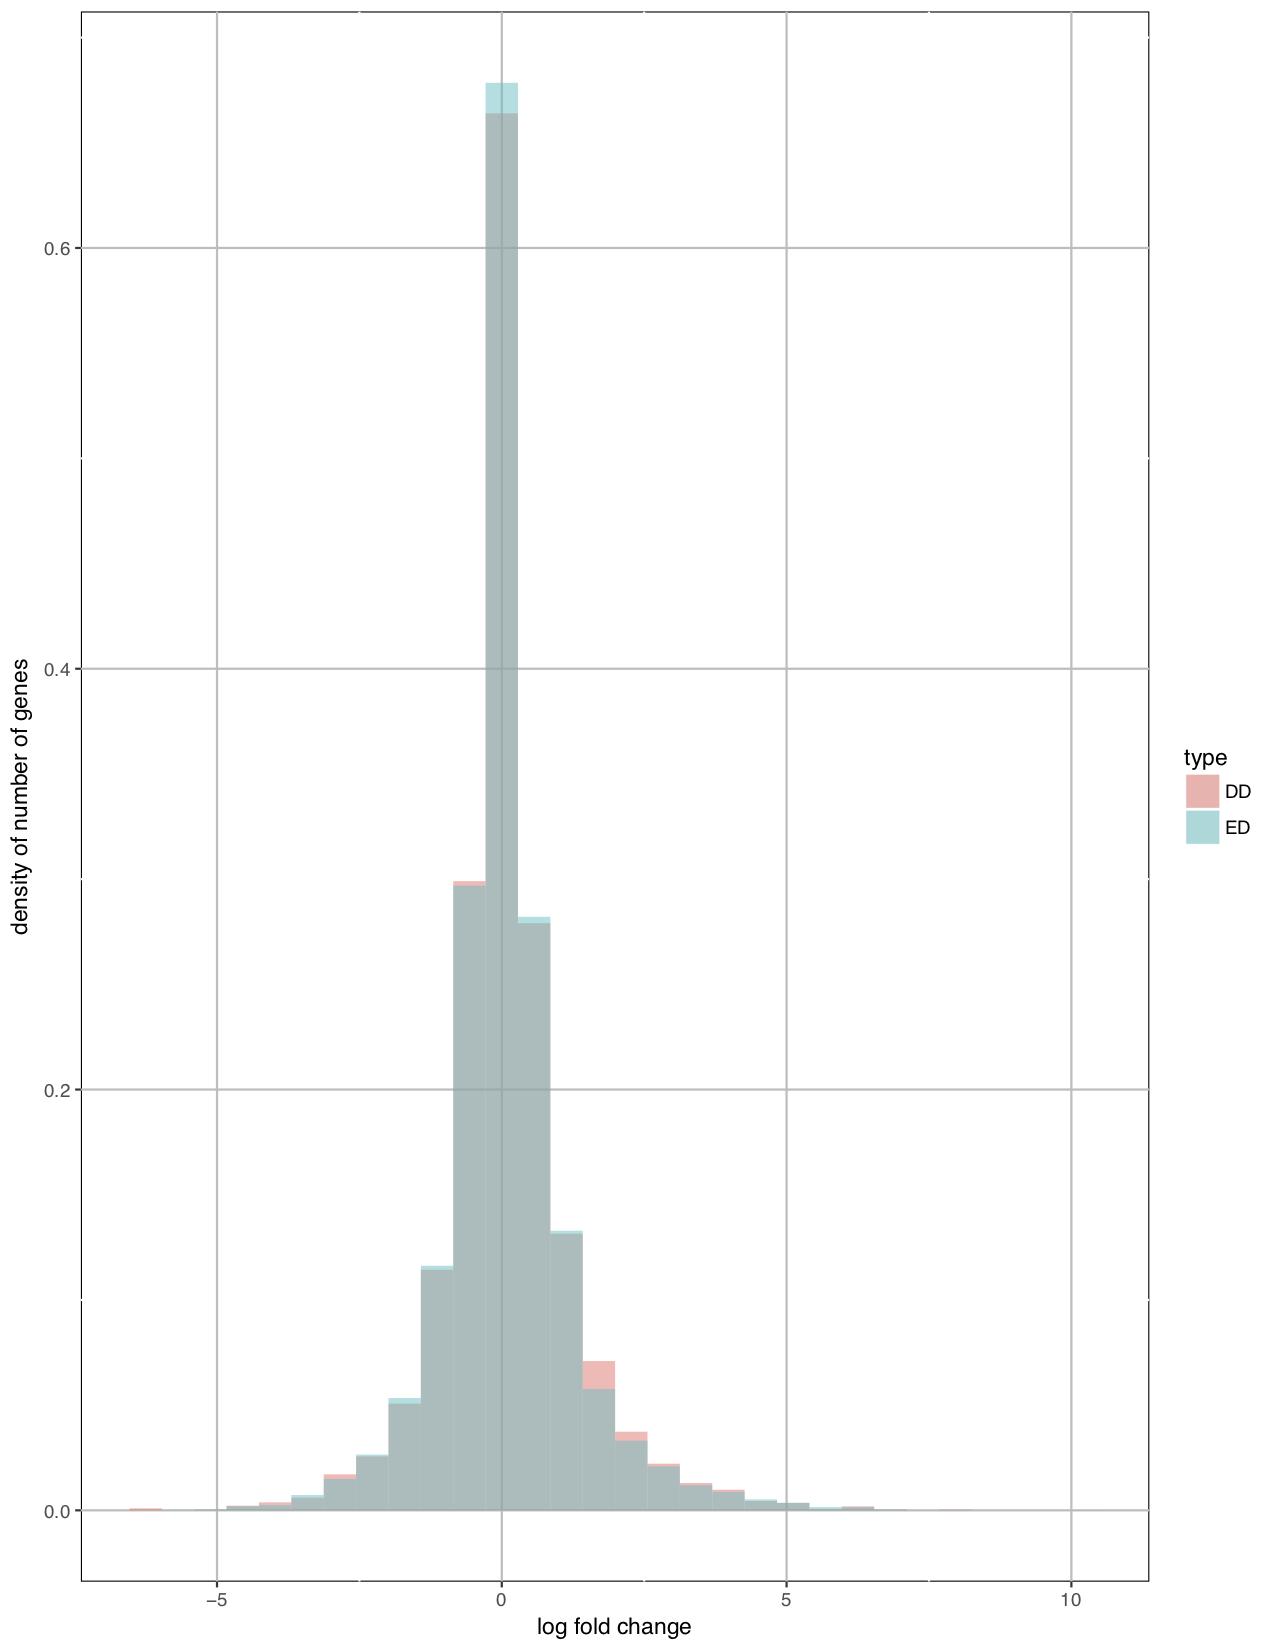
\includegraphics[width=\linewidth]{DEC_NPC_mast.png}
  \caption{MAST}
\endminipage\hfill
\minipage{0.25\textwidth}
  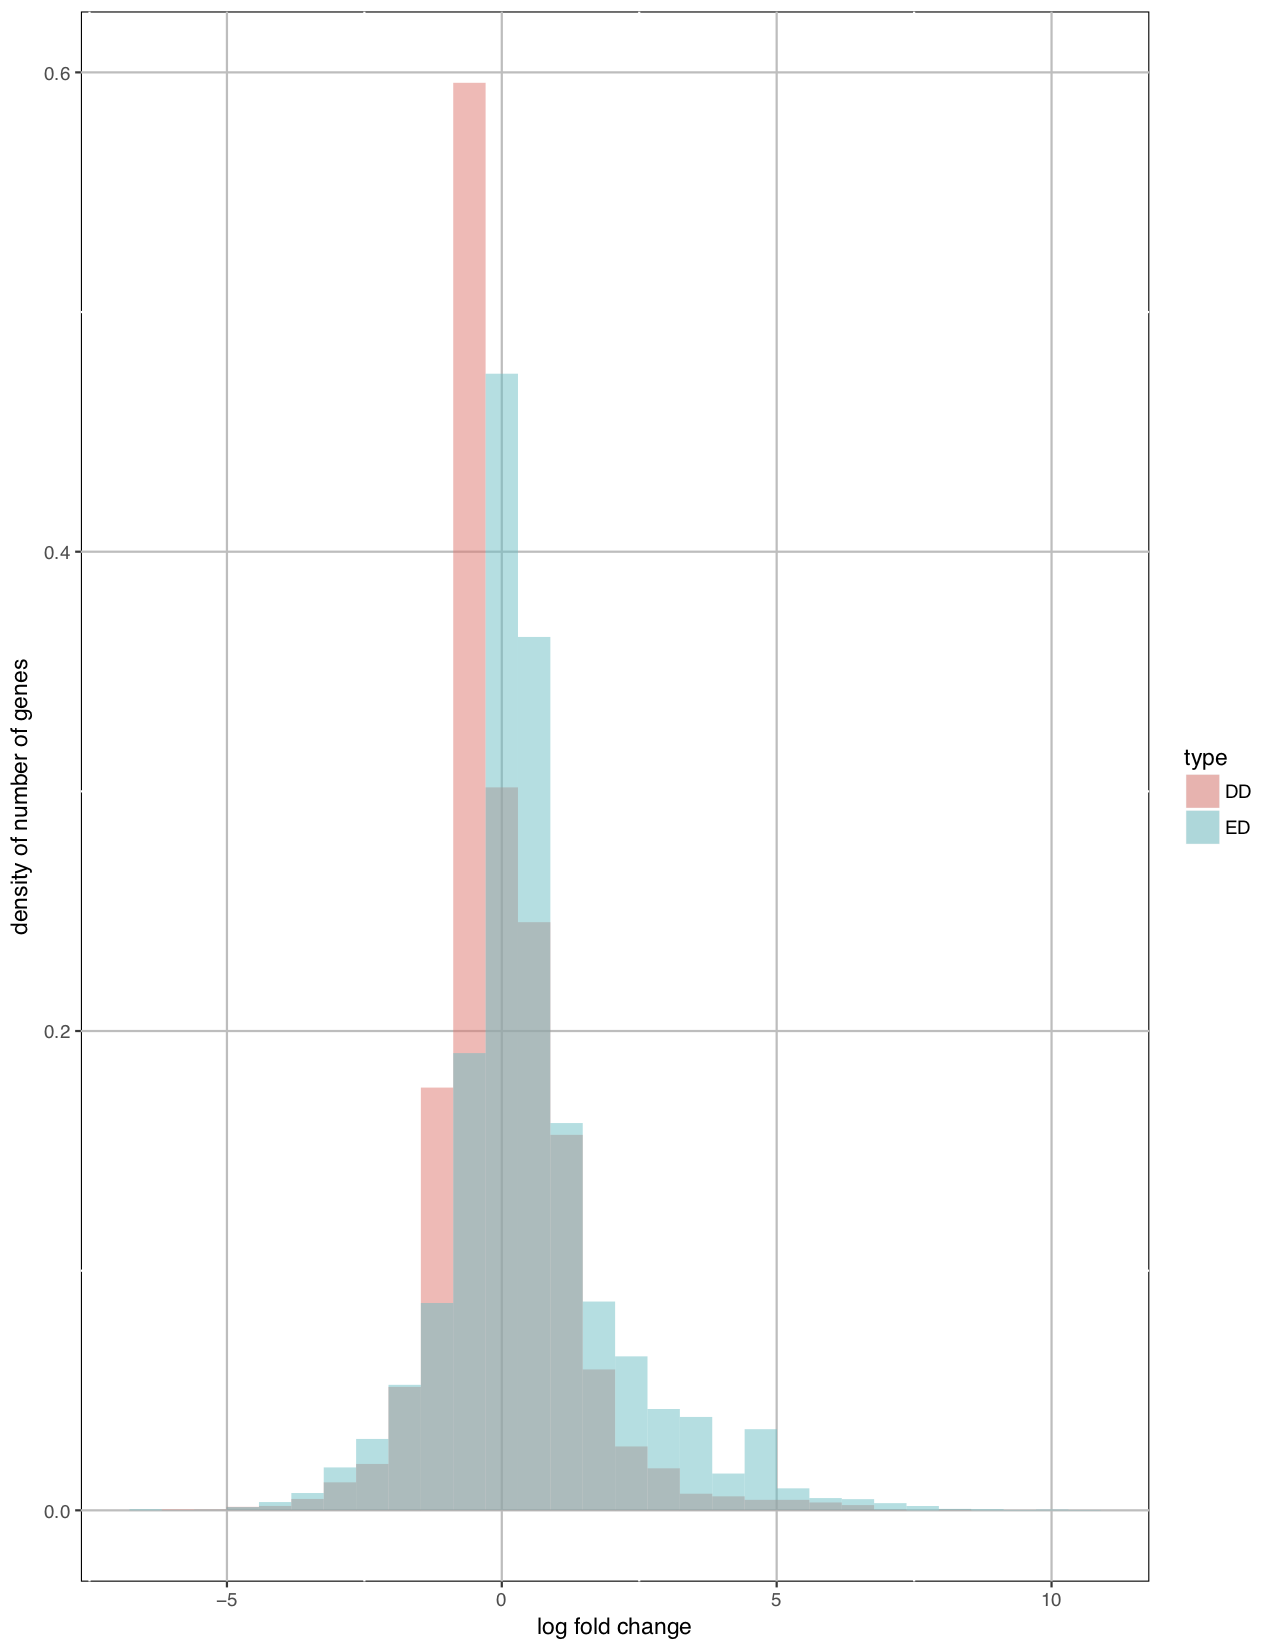
\includegraphics[width=\linewidth]{DEC_NPC_scdd.png}
  \caption{scDD}\label{fig:scDD}
\endminipage\hfill
\minipage{0.25\textwidth}
  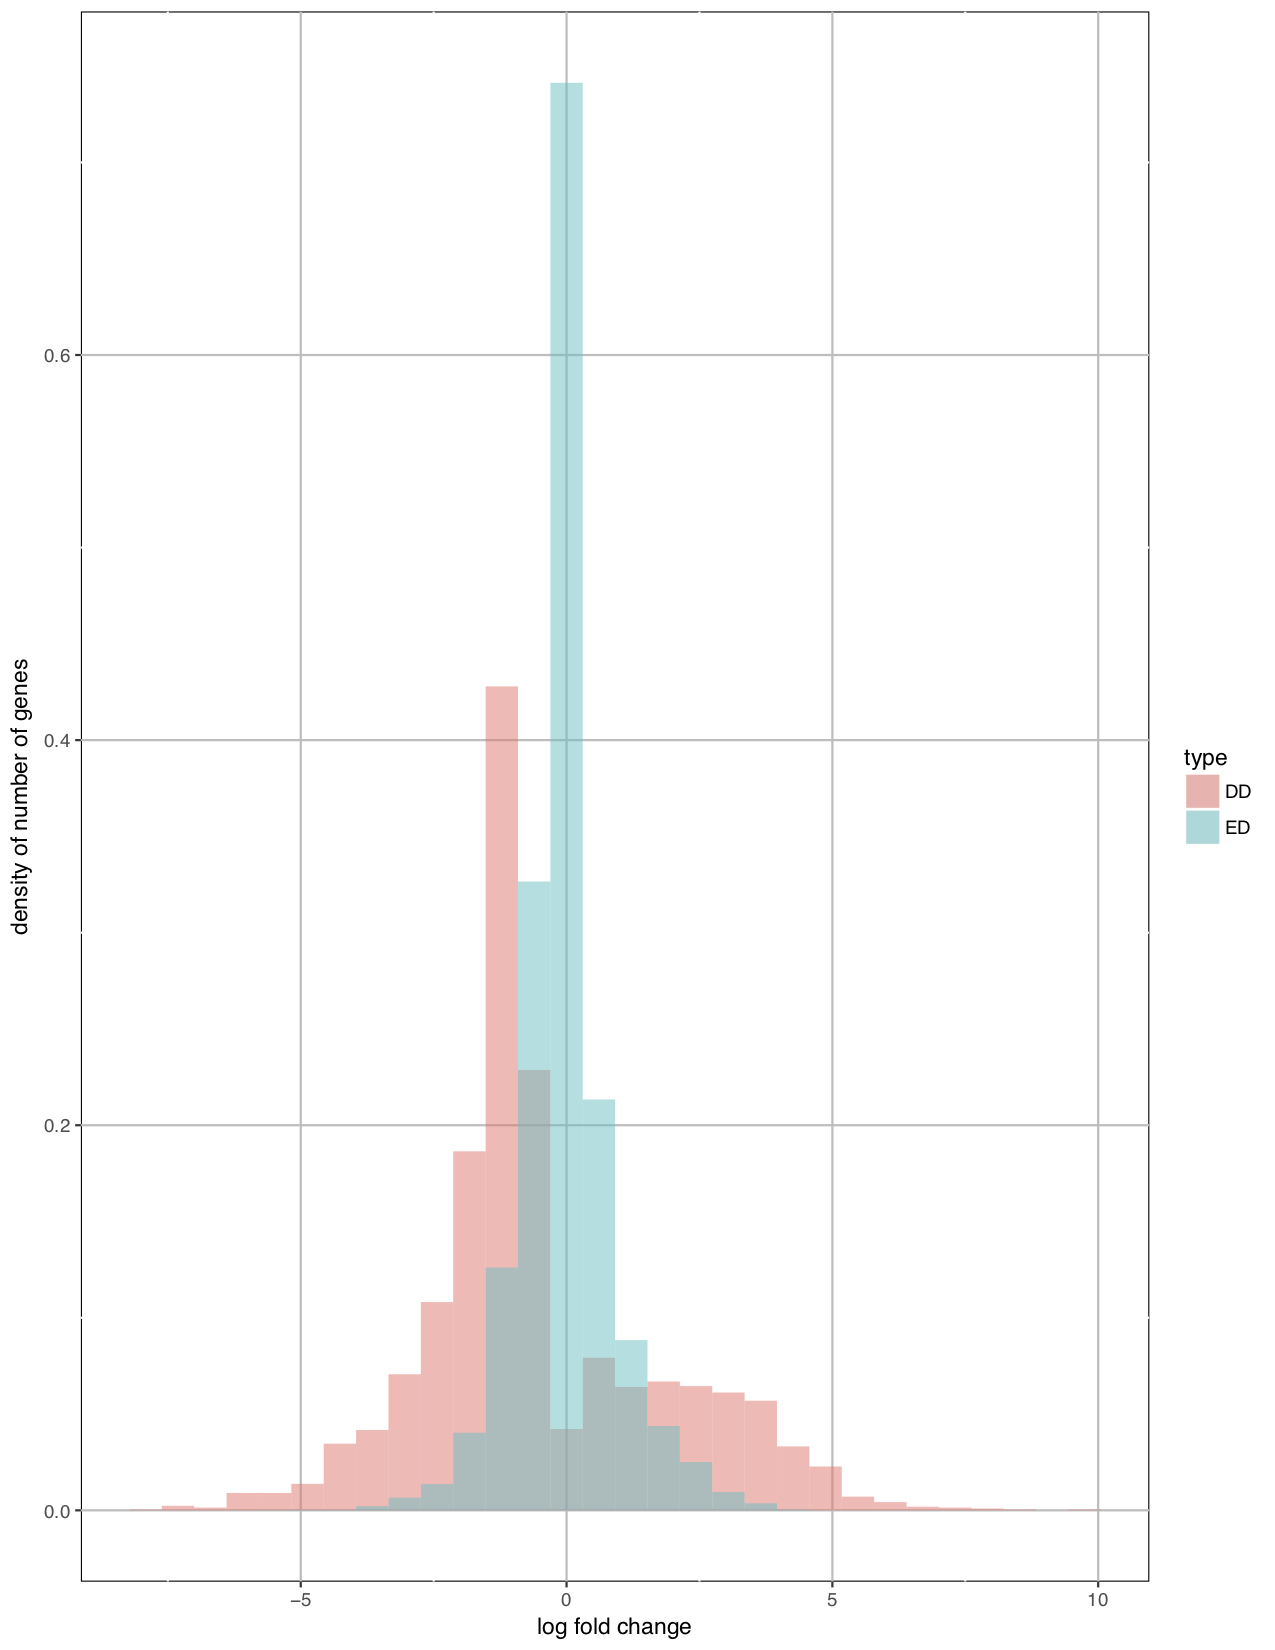
\includegraphics[width=\linewidth]{DEC_NPC_scddb.png}
  \caption{scDDboost}\label{fig:scDDboost}
\endminipage\hfill
\minipage{0.25\textwidth}%
  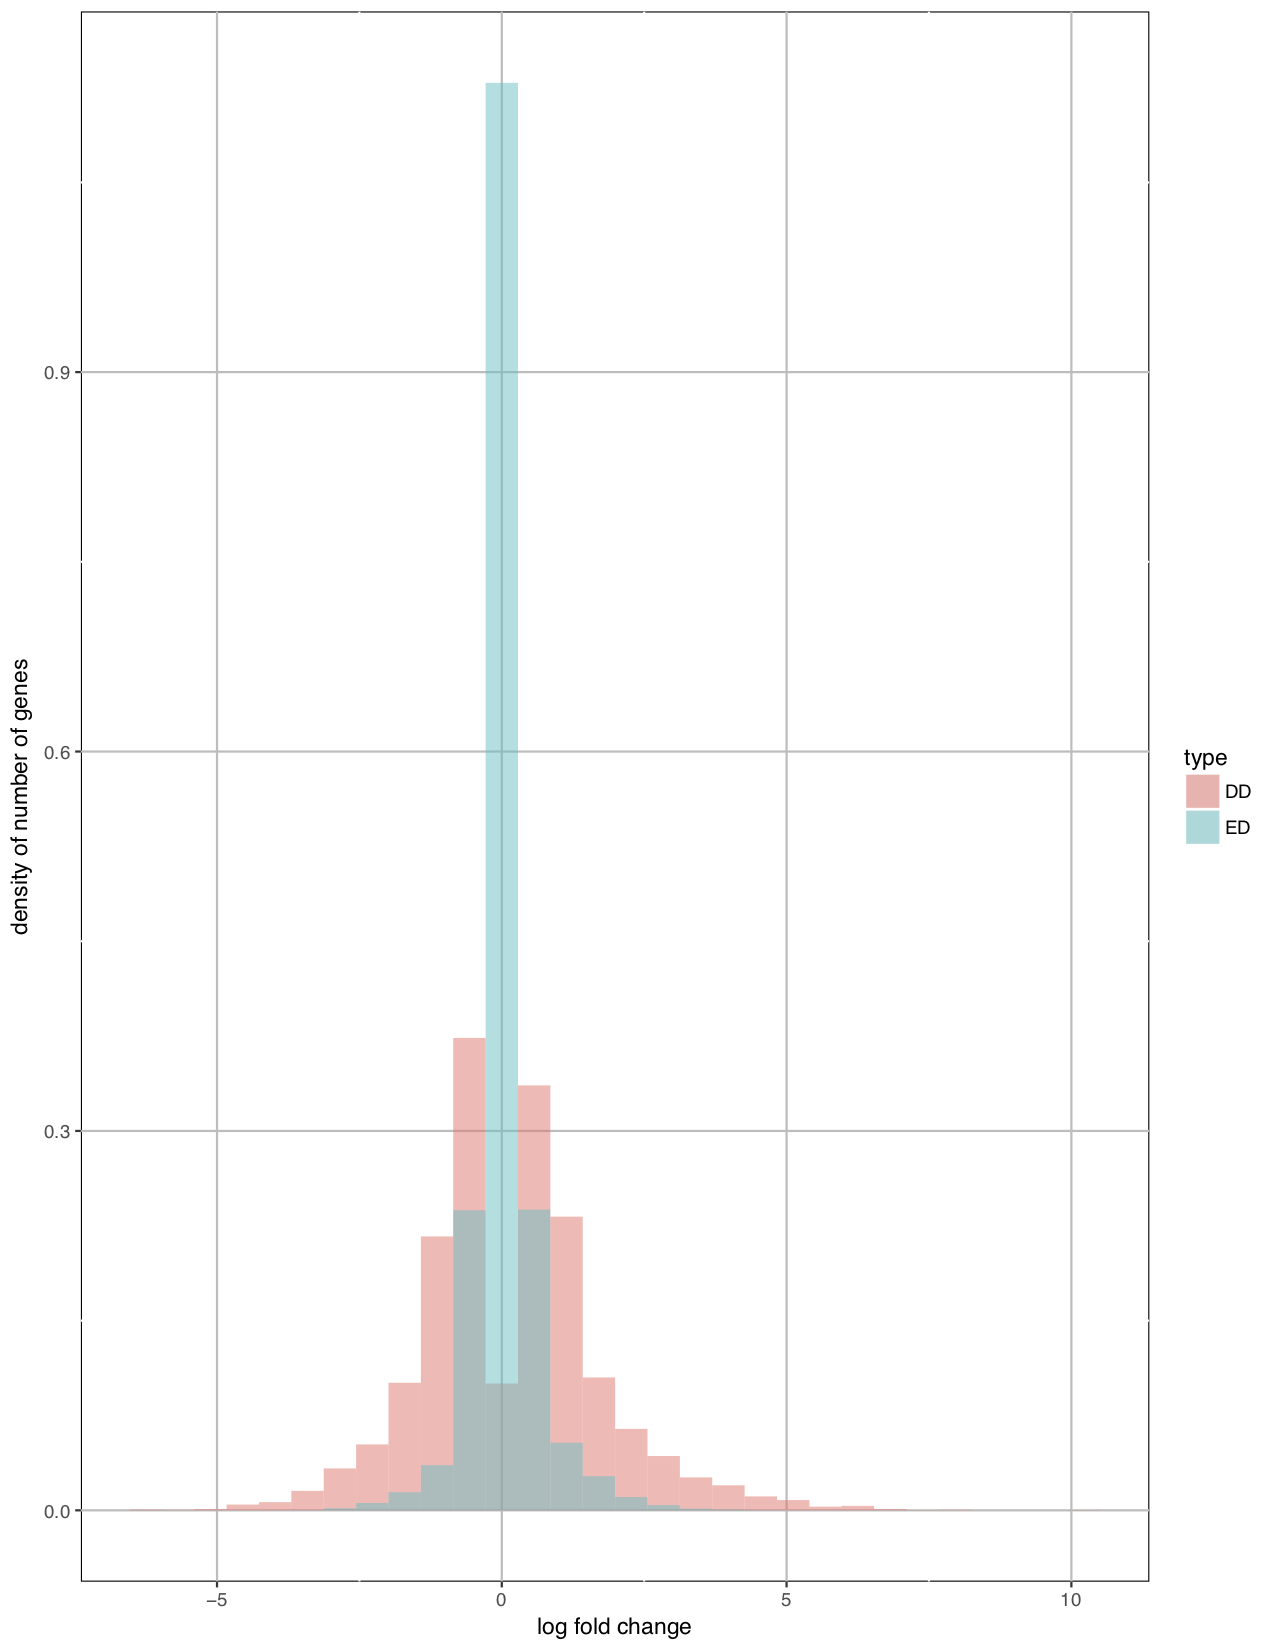
\includegraphics[width=\linewidth]{DEC_NPC_des.png}
  \caption{DESeq2}\label{fig:DESeq2}
\endminipage
\end{figure}

\begin{figure}[ht]
\minipage{0.25\textwidth}
  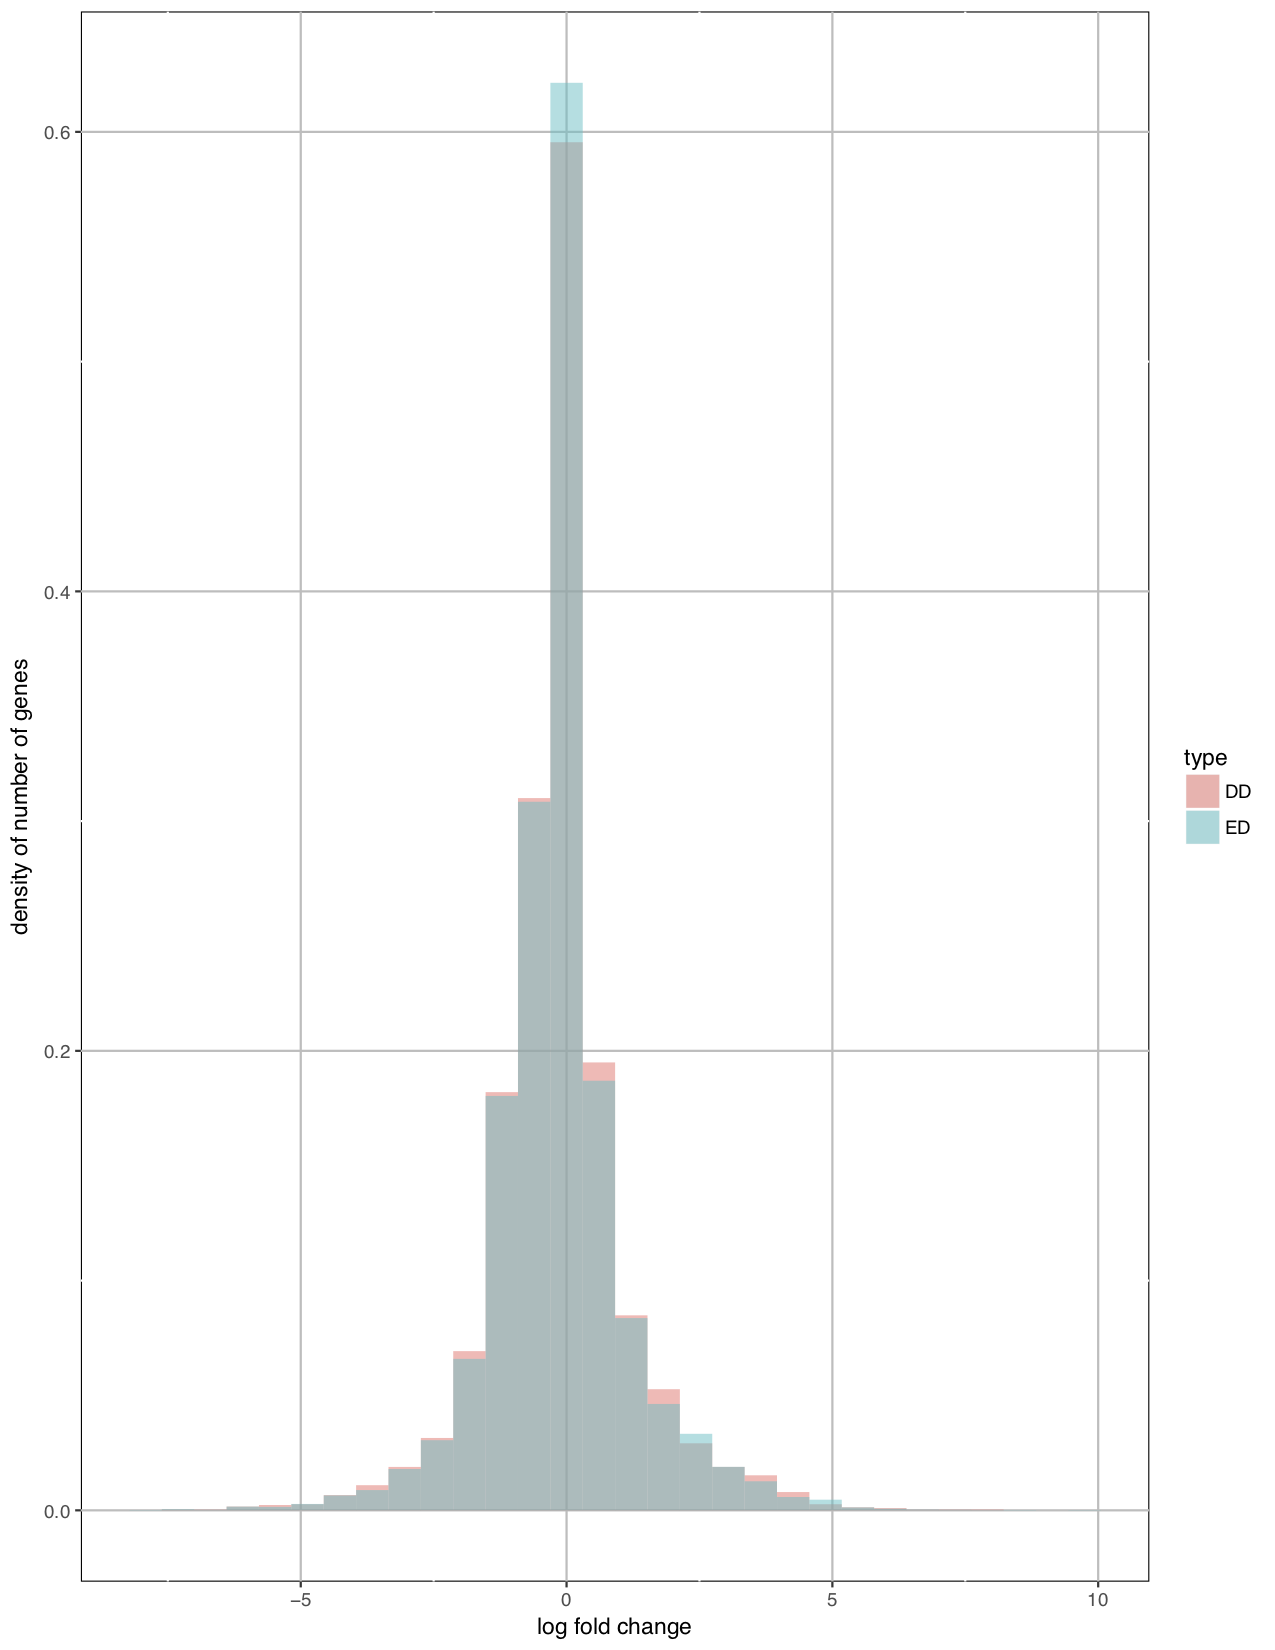
\includegraphics[width=\linewidth]{DEC_EC_mast.png}
  \caption{MAST}
\endminipage\hfill
\minipage{0.25\textwidth}
  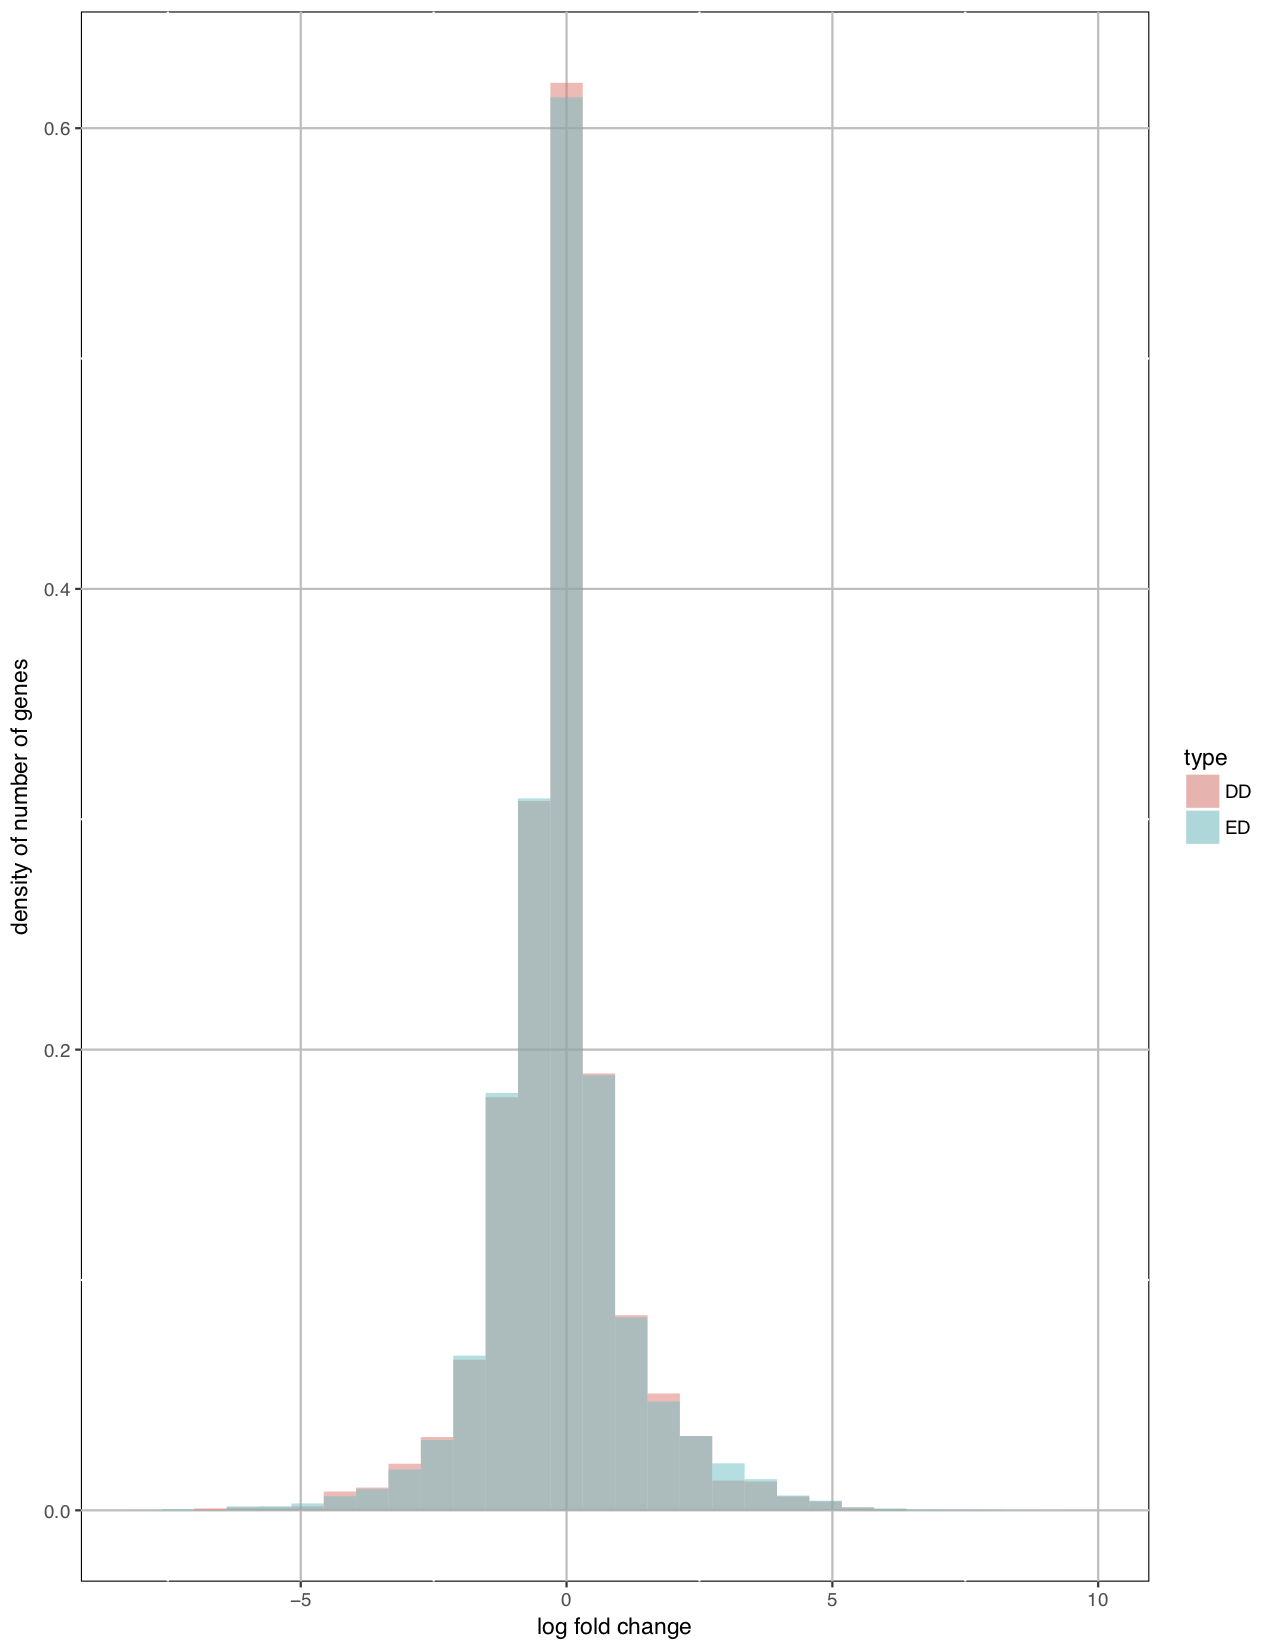
\includegraphics[width=\linewidth]{DEC_EC_scdd.png}
  \caption{scDD}\label{fig:scDD}
\endminipage\hfill
\minipage{0.25\textwidth}
  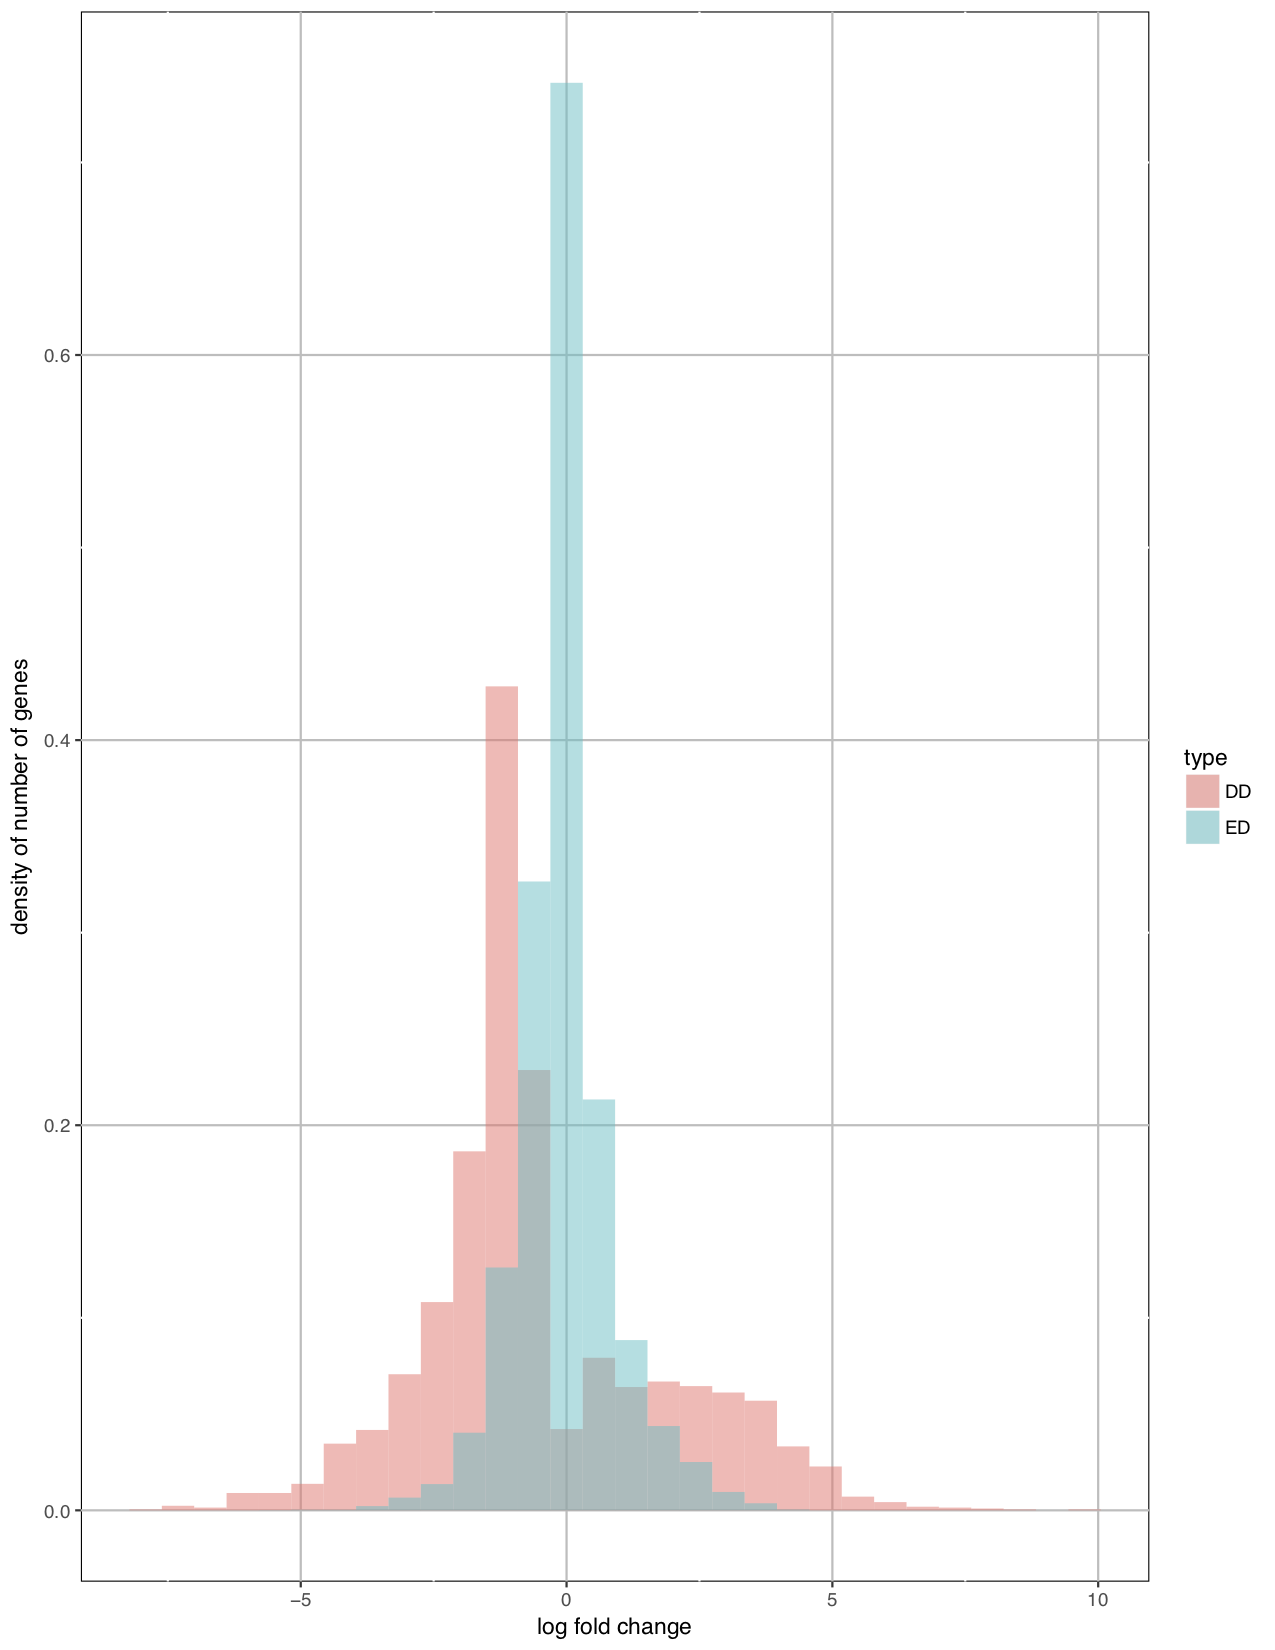
\includegraphics[width=\linewidth]{DEC_EC_scddb.png}
  \caption{scDDboost}\label{fig:scDDboost}
\endminipage\hfill
\minipage{0.25\textwidth}%
  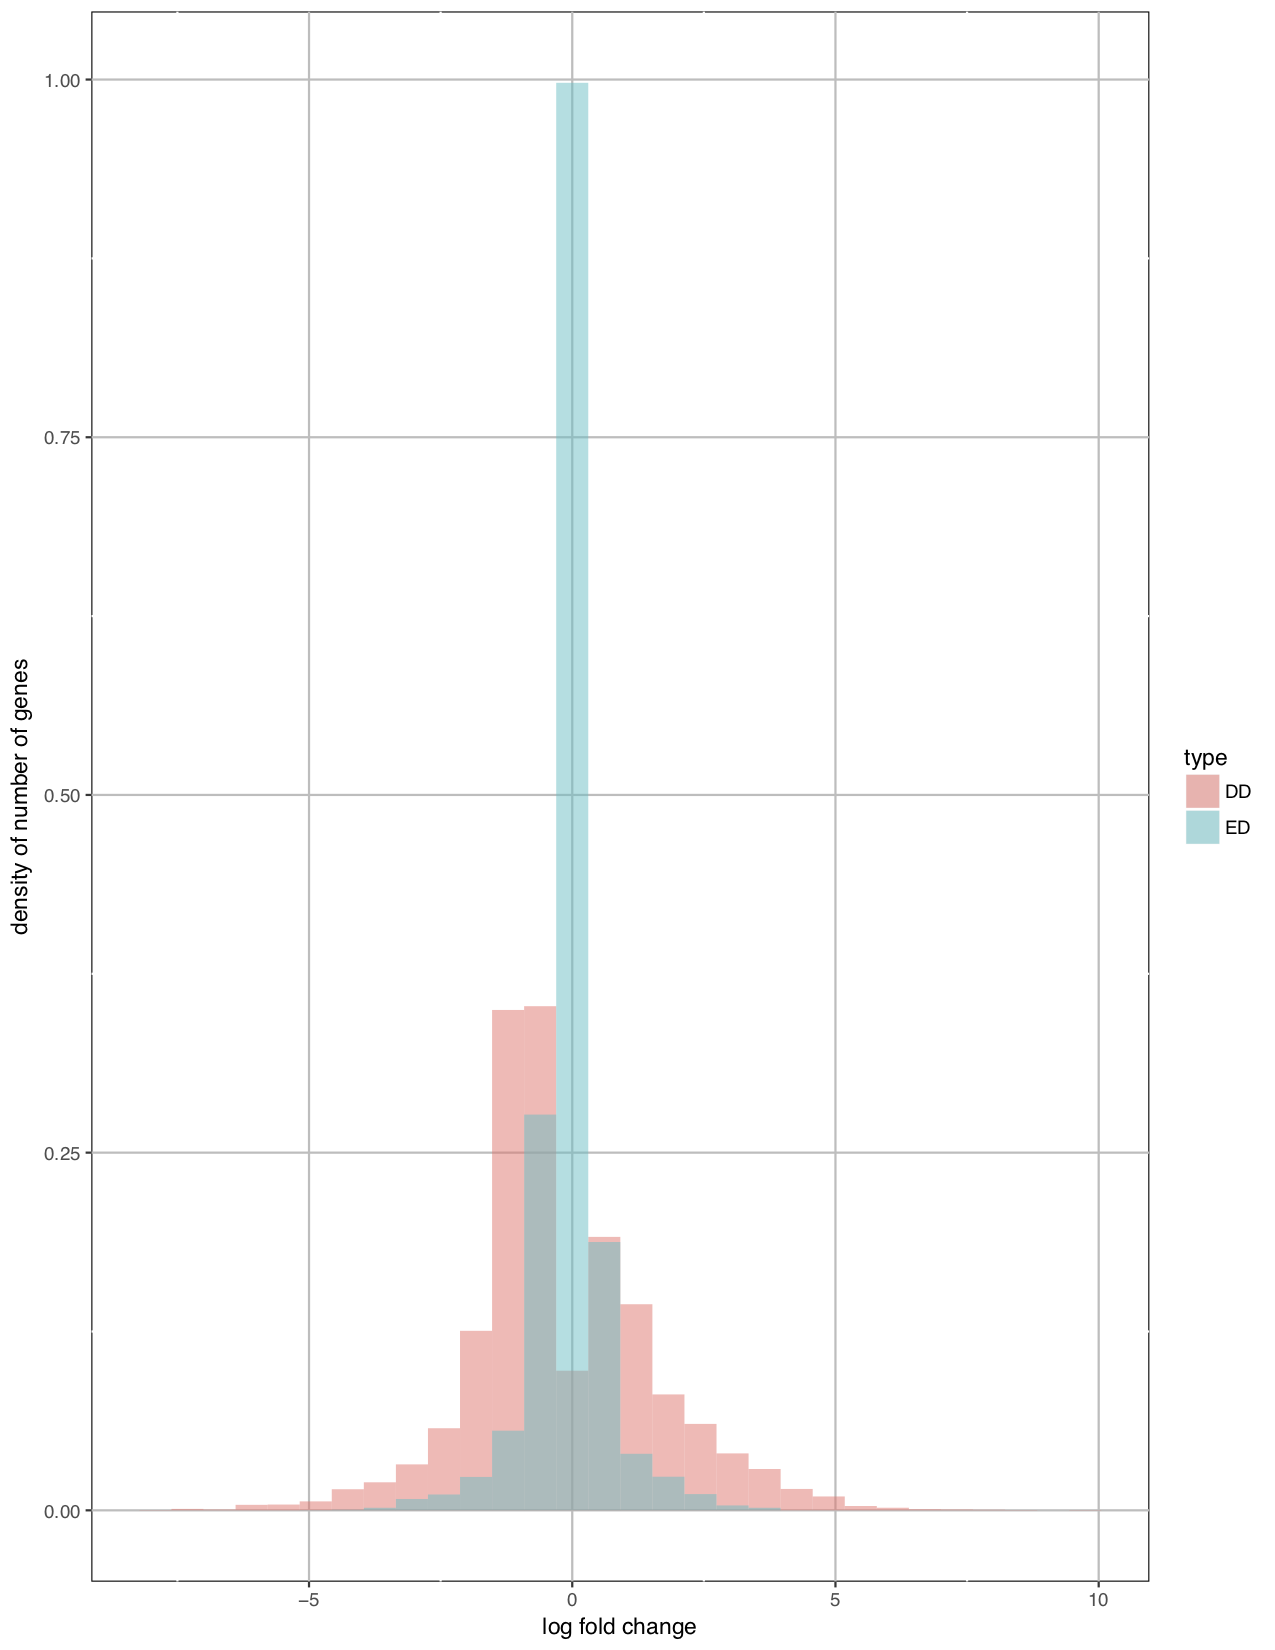
\includegraphics[width=\linewidth]{DEC_EC_des.png}
  \caption{DESeq2}\label{fig:DESeq2}
\endminipage
\end{figure}

\begin{figure}[H]
\minipage{0.25\textwidth}
  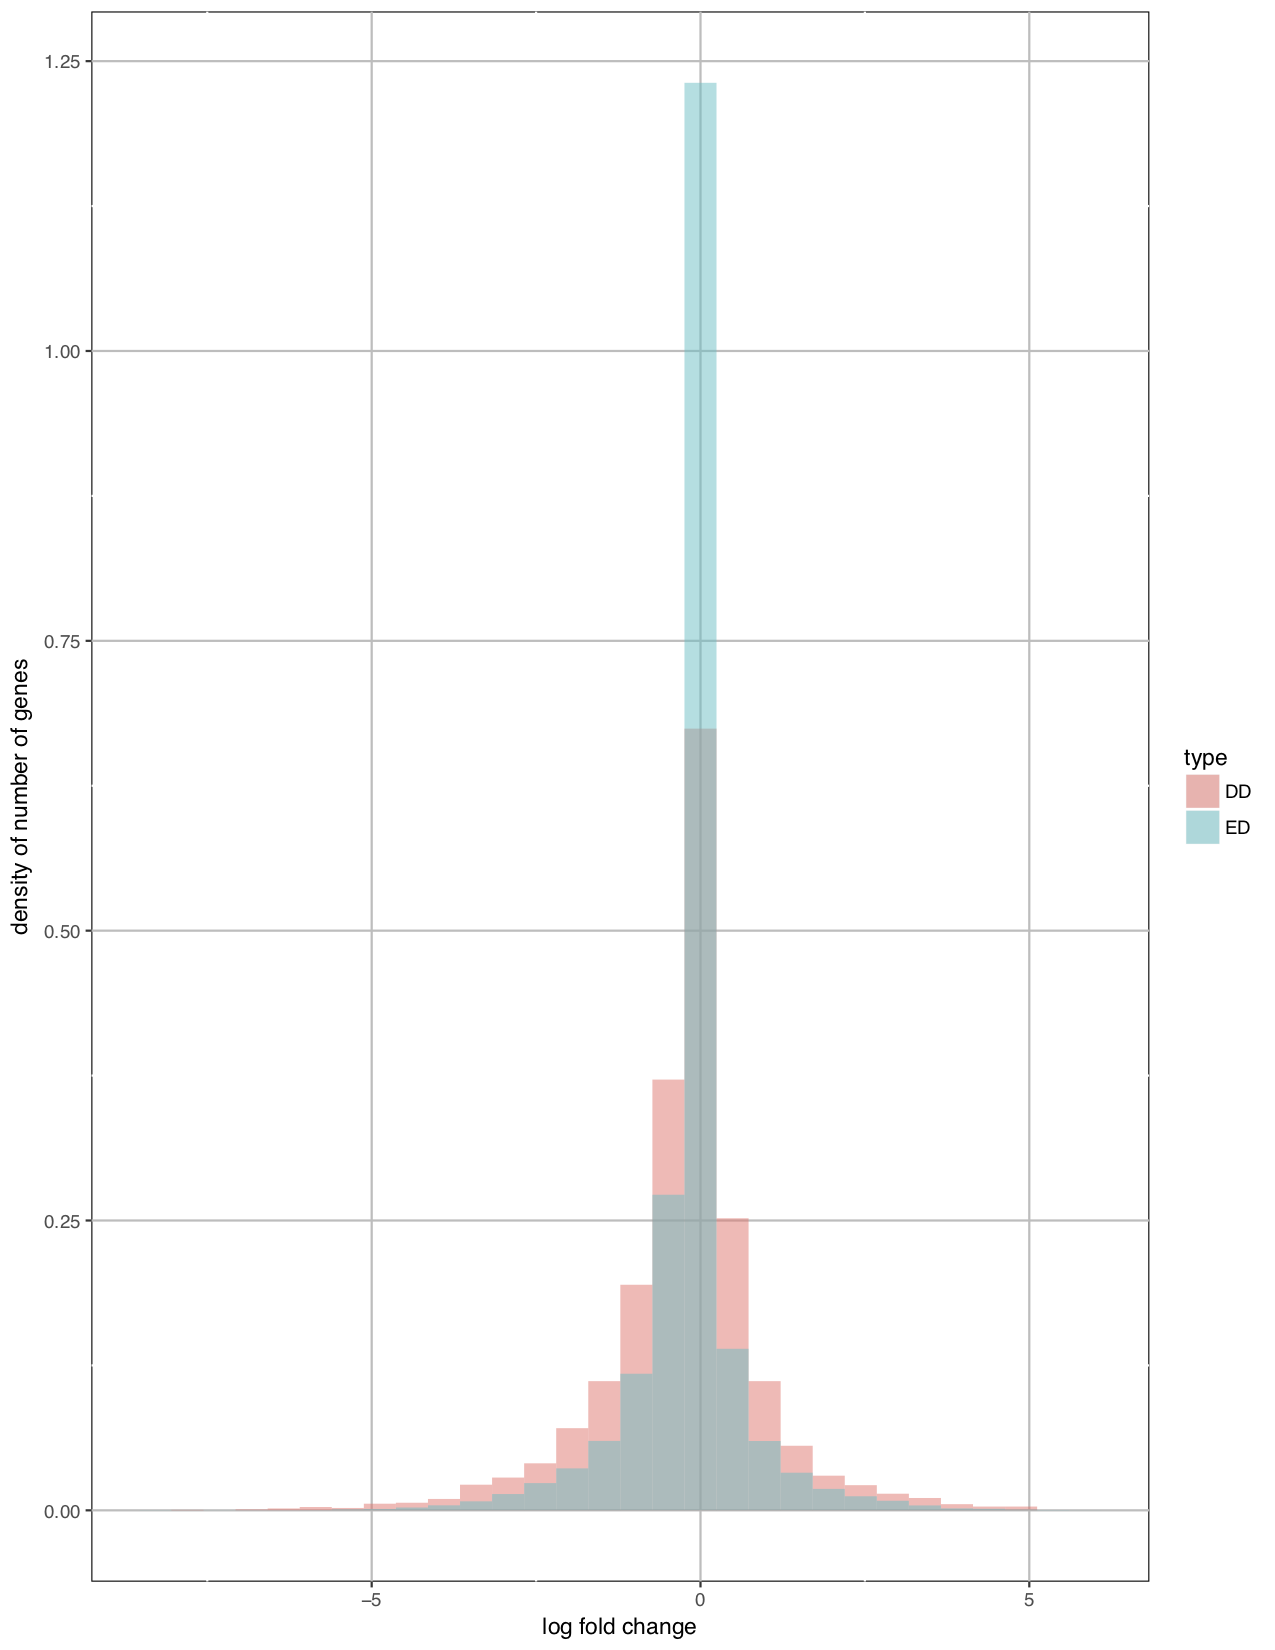
\includegraphics[width=\linewidth]{G45719_mast.png}
  \caption{MAST}
\endminipage\hfill
\minipage{0.25\textwidth}
  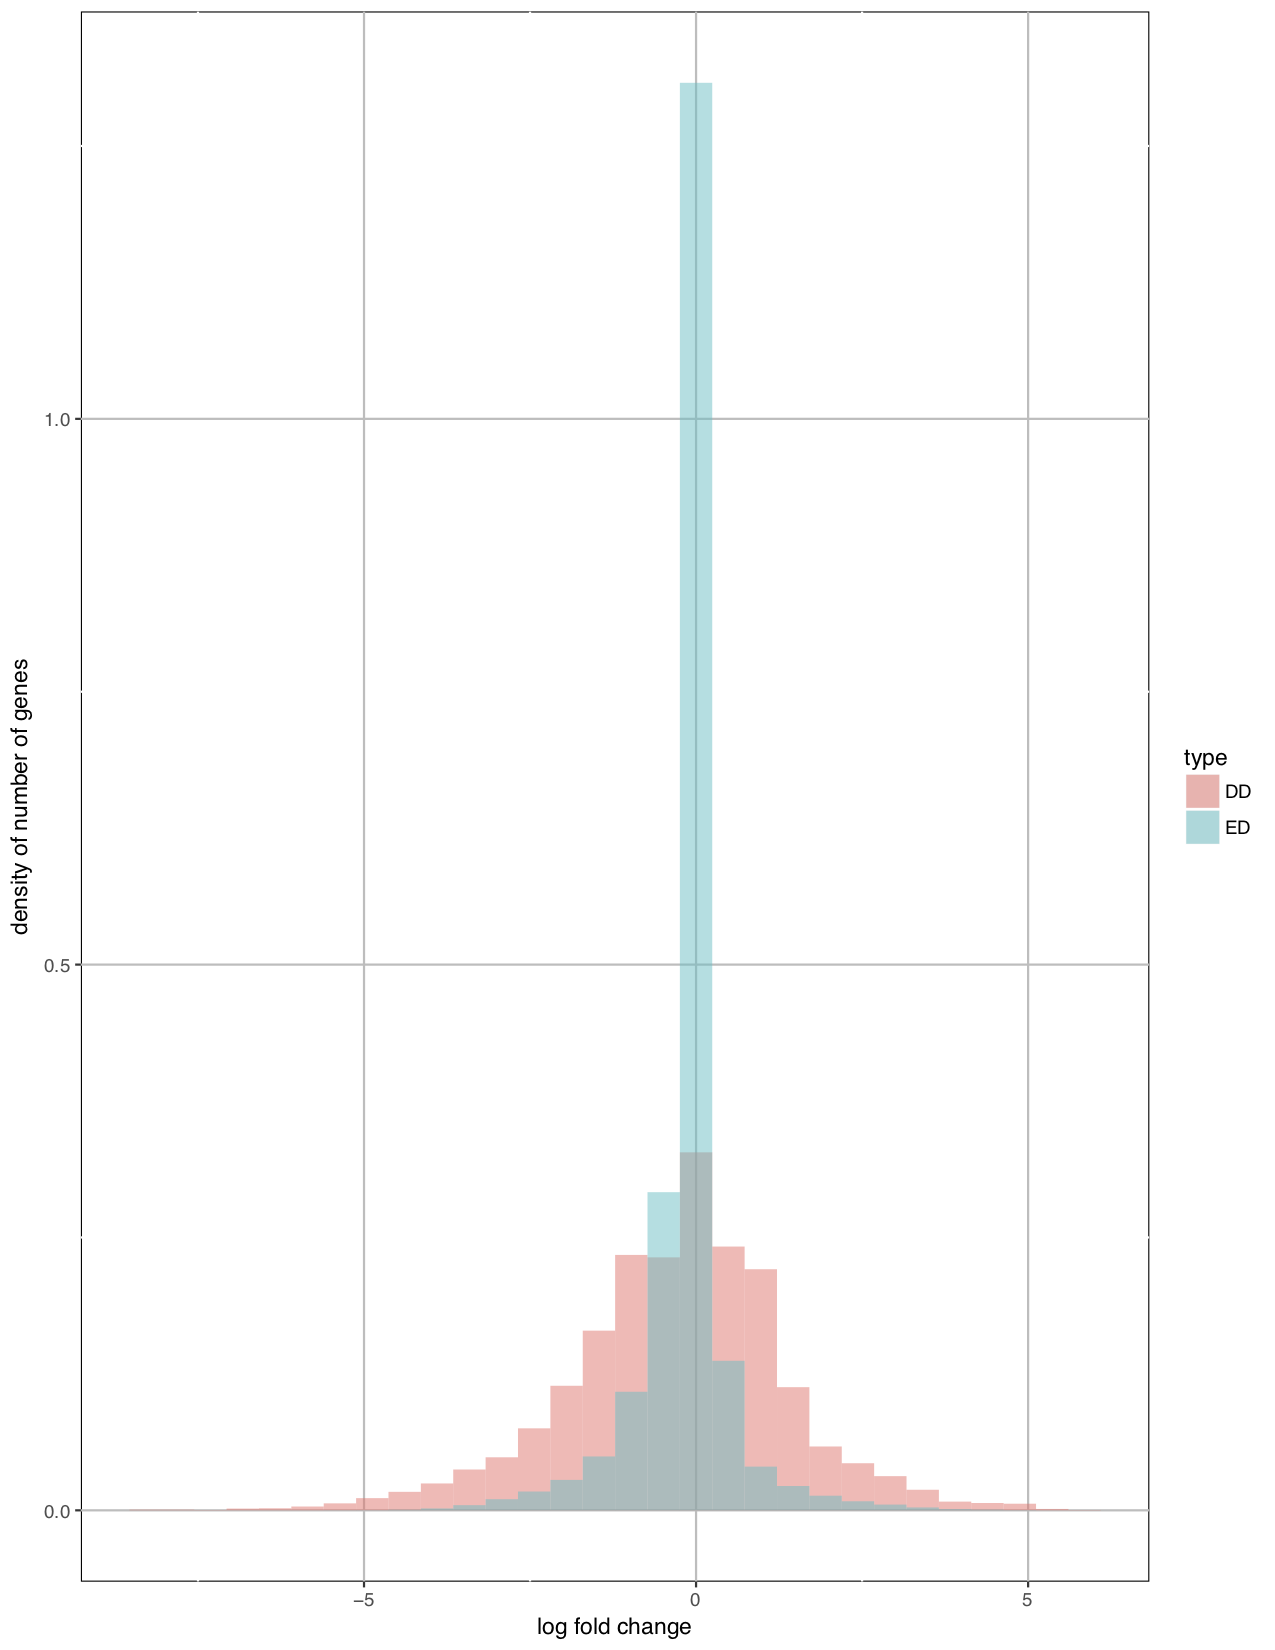
\includegraphics[width=\linewidth]{G45719_scdd.png}
  \caption{scDD}\label{fig:scDD}
\endminipage\hfill
\minipage{0.25\textwidth}
  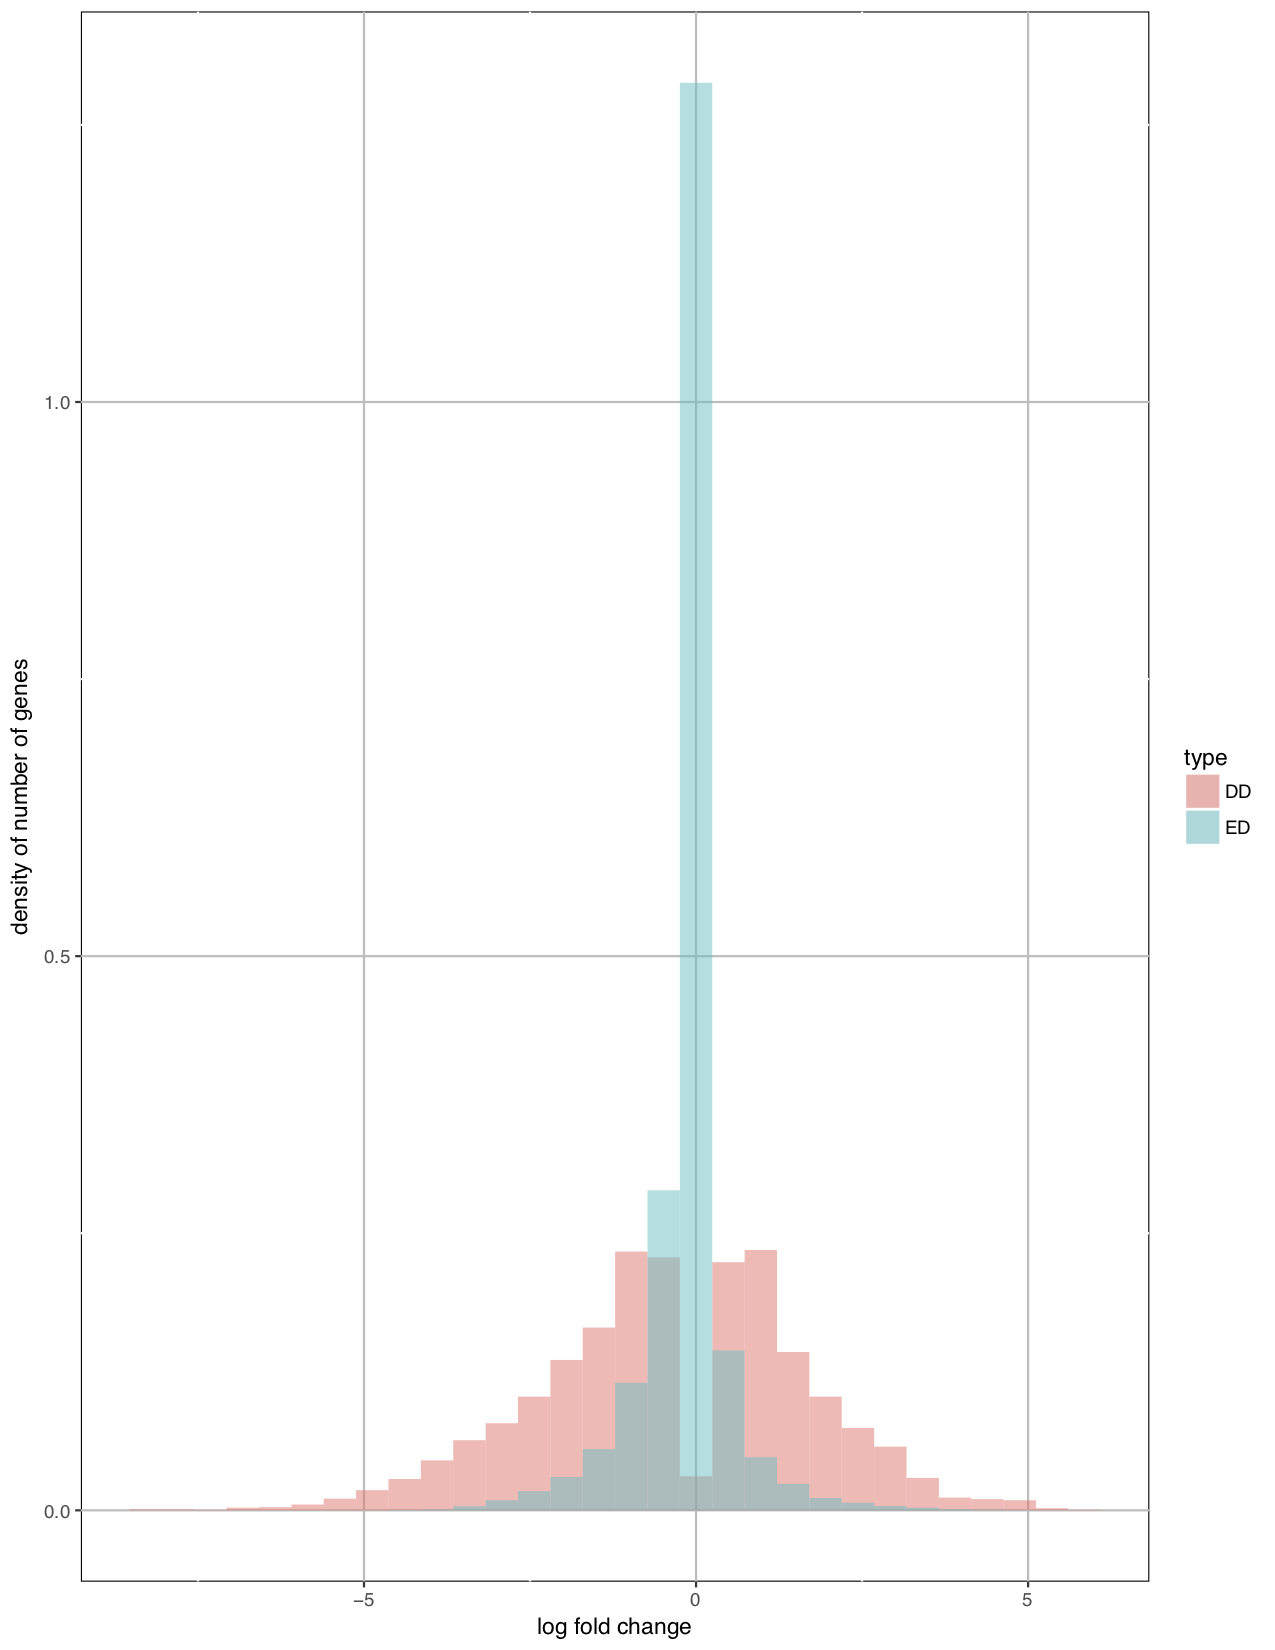
\includegraphics[width=\linewidth]{G45719_scddb.png}
  \caption{scDDboost}\label{fig:scDDboost}
\endminipage\hfill
\minipage{0.25\textwidth}%
  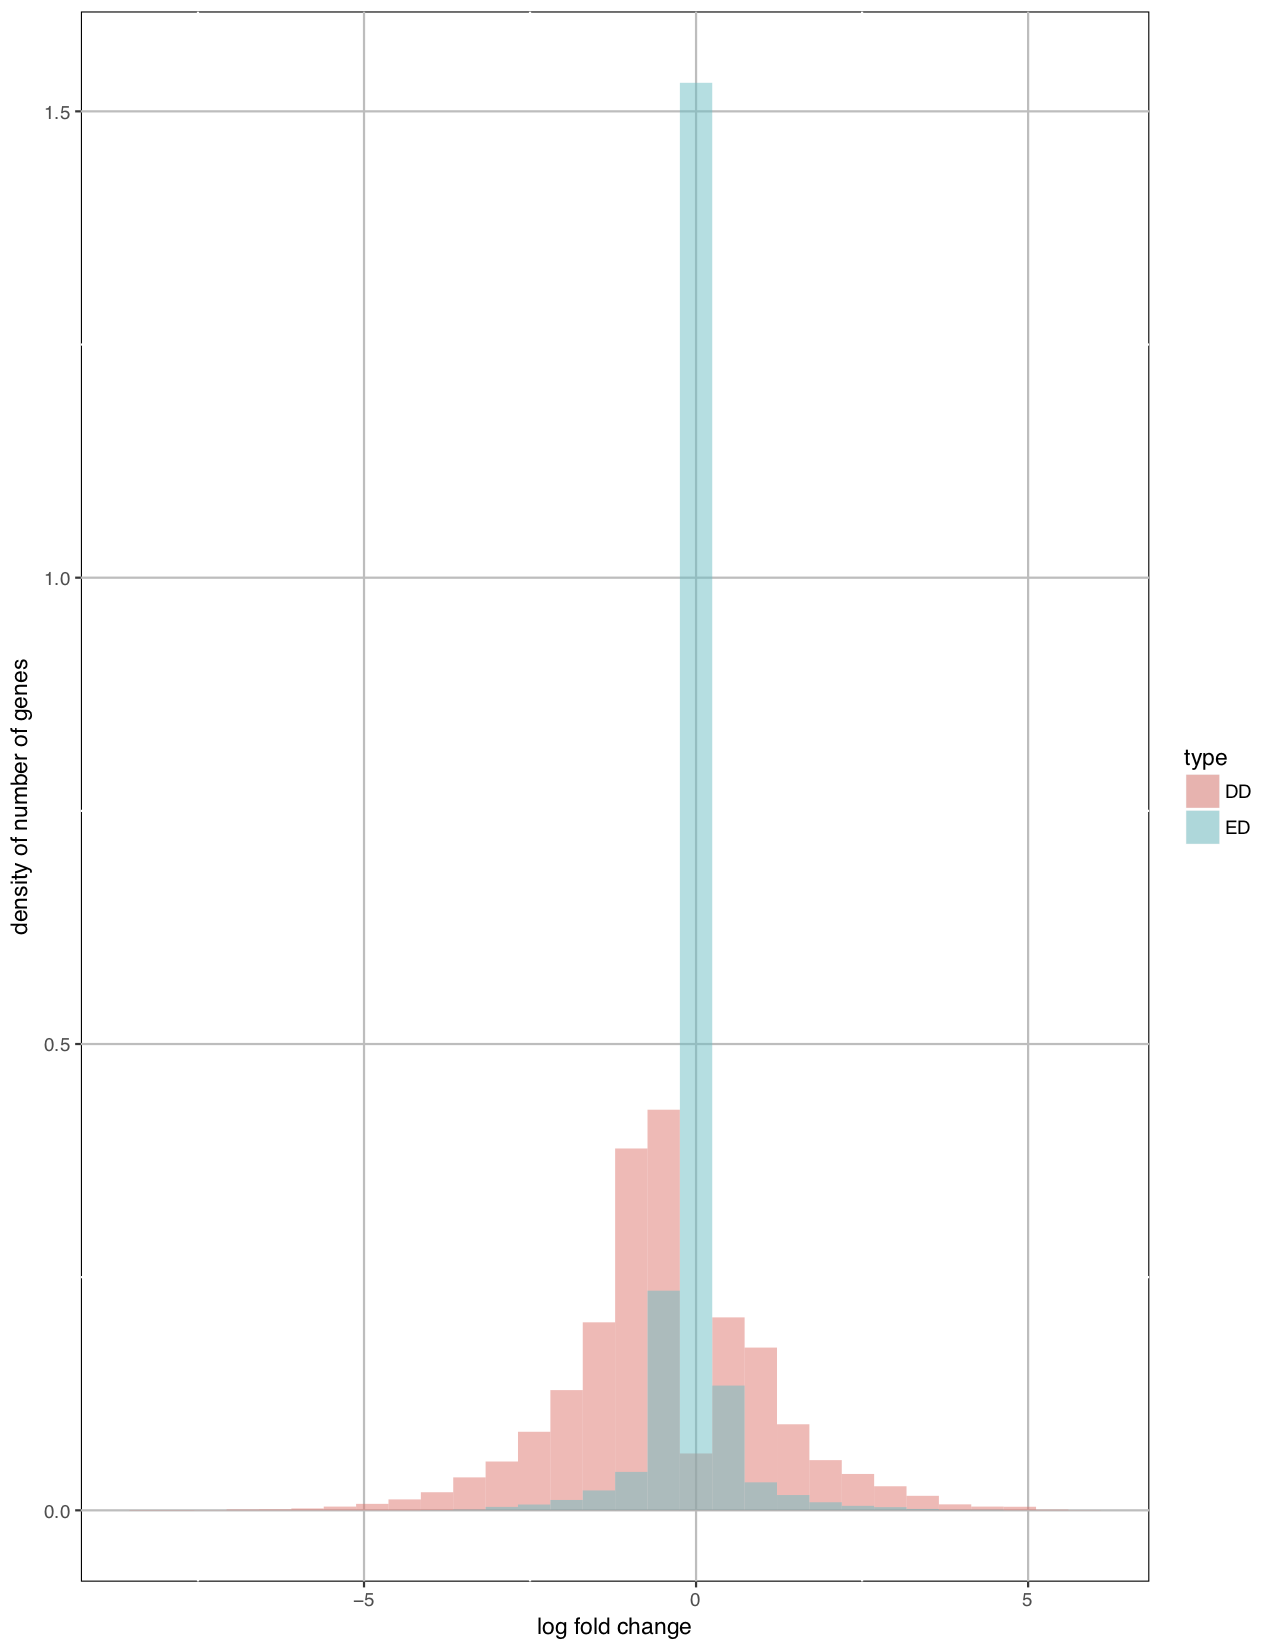
\includegraphics[width=\linewidth]{G45719_des.png}
  \caption{DESeq2}\label{fig:DESeq2}
\endminipage
\end{figure}

\begin{figure}[H]
\minipage{0.25\textwidth}
  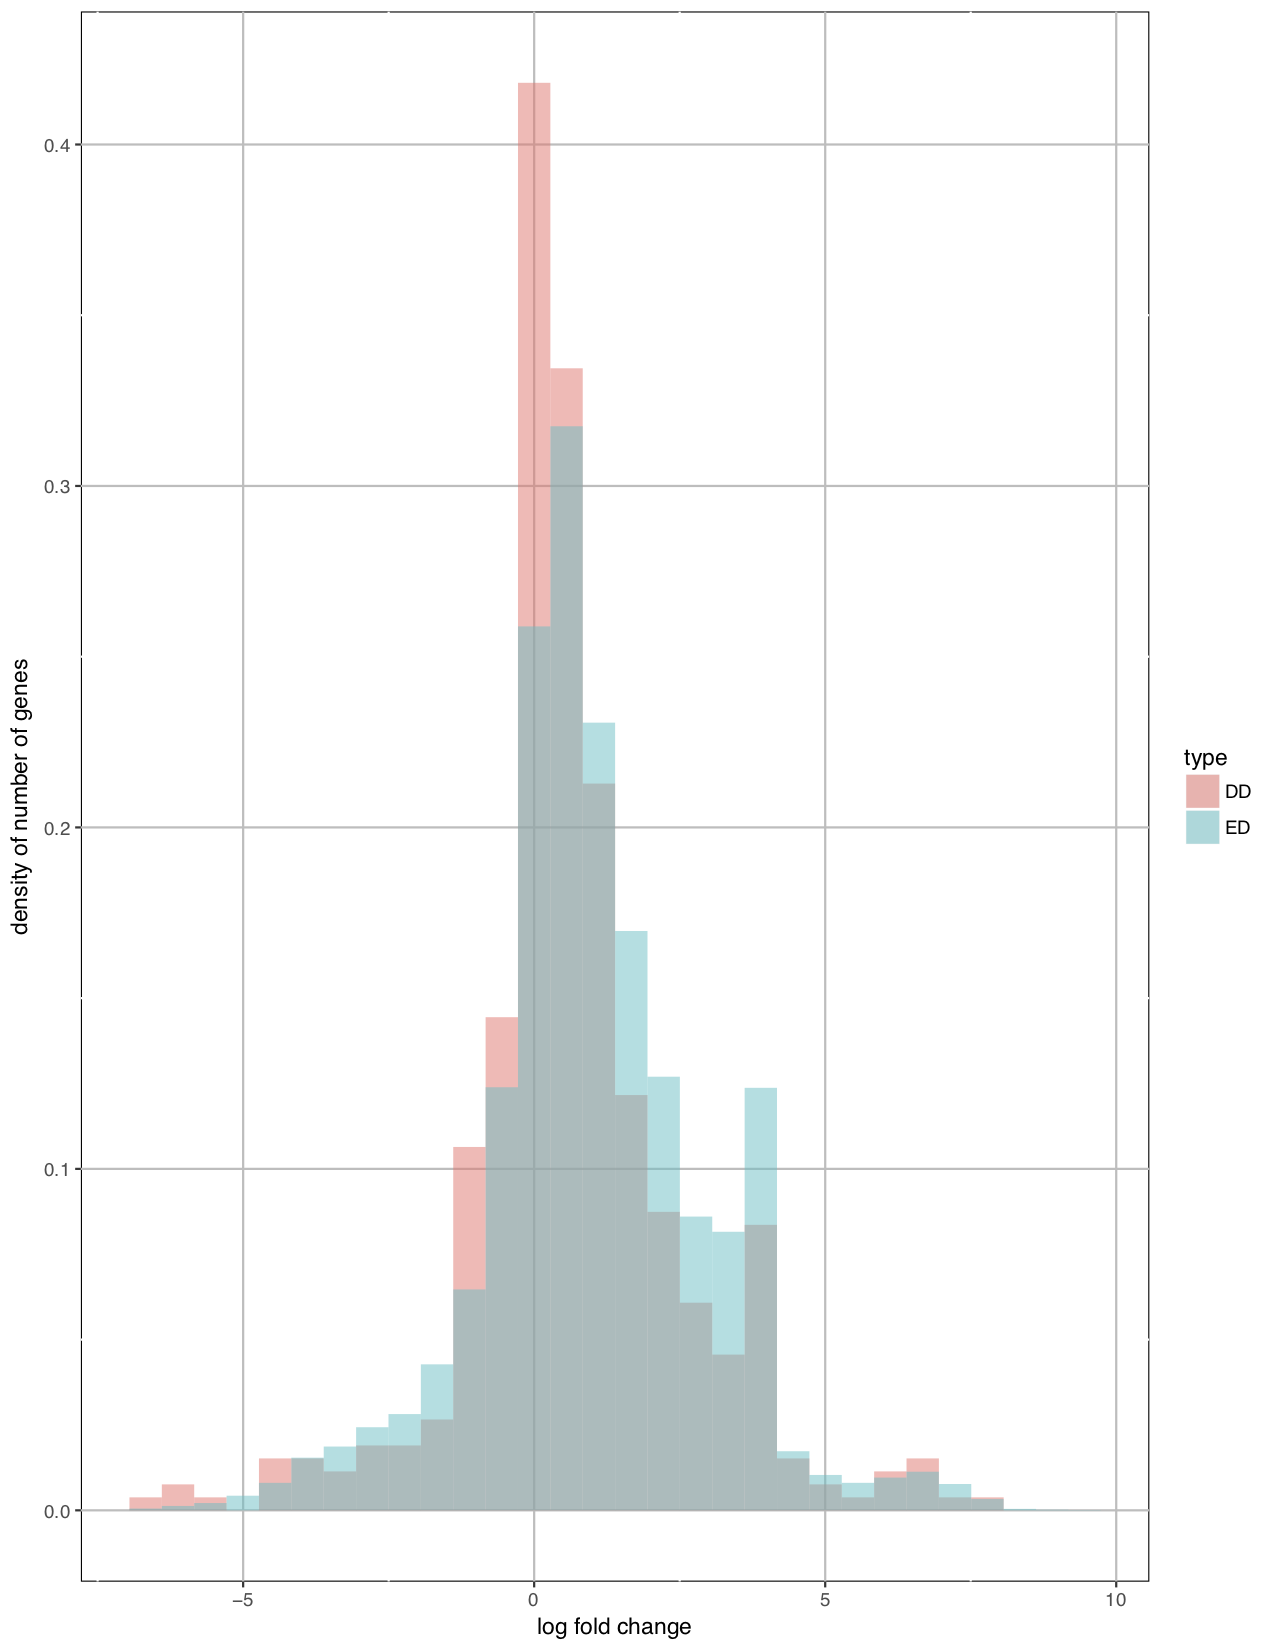
\includegraphics[width=\linewidth]{G74596_mast.png}
  \caption{MAST}
\endminipage\hfill
\minipage{0.25\textwidth}
  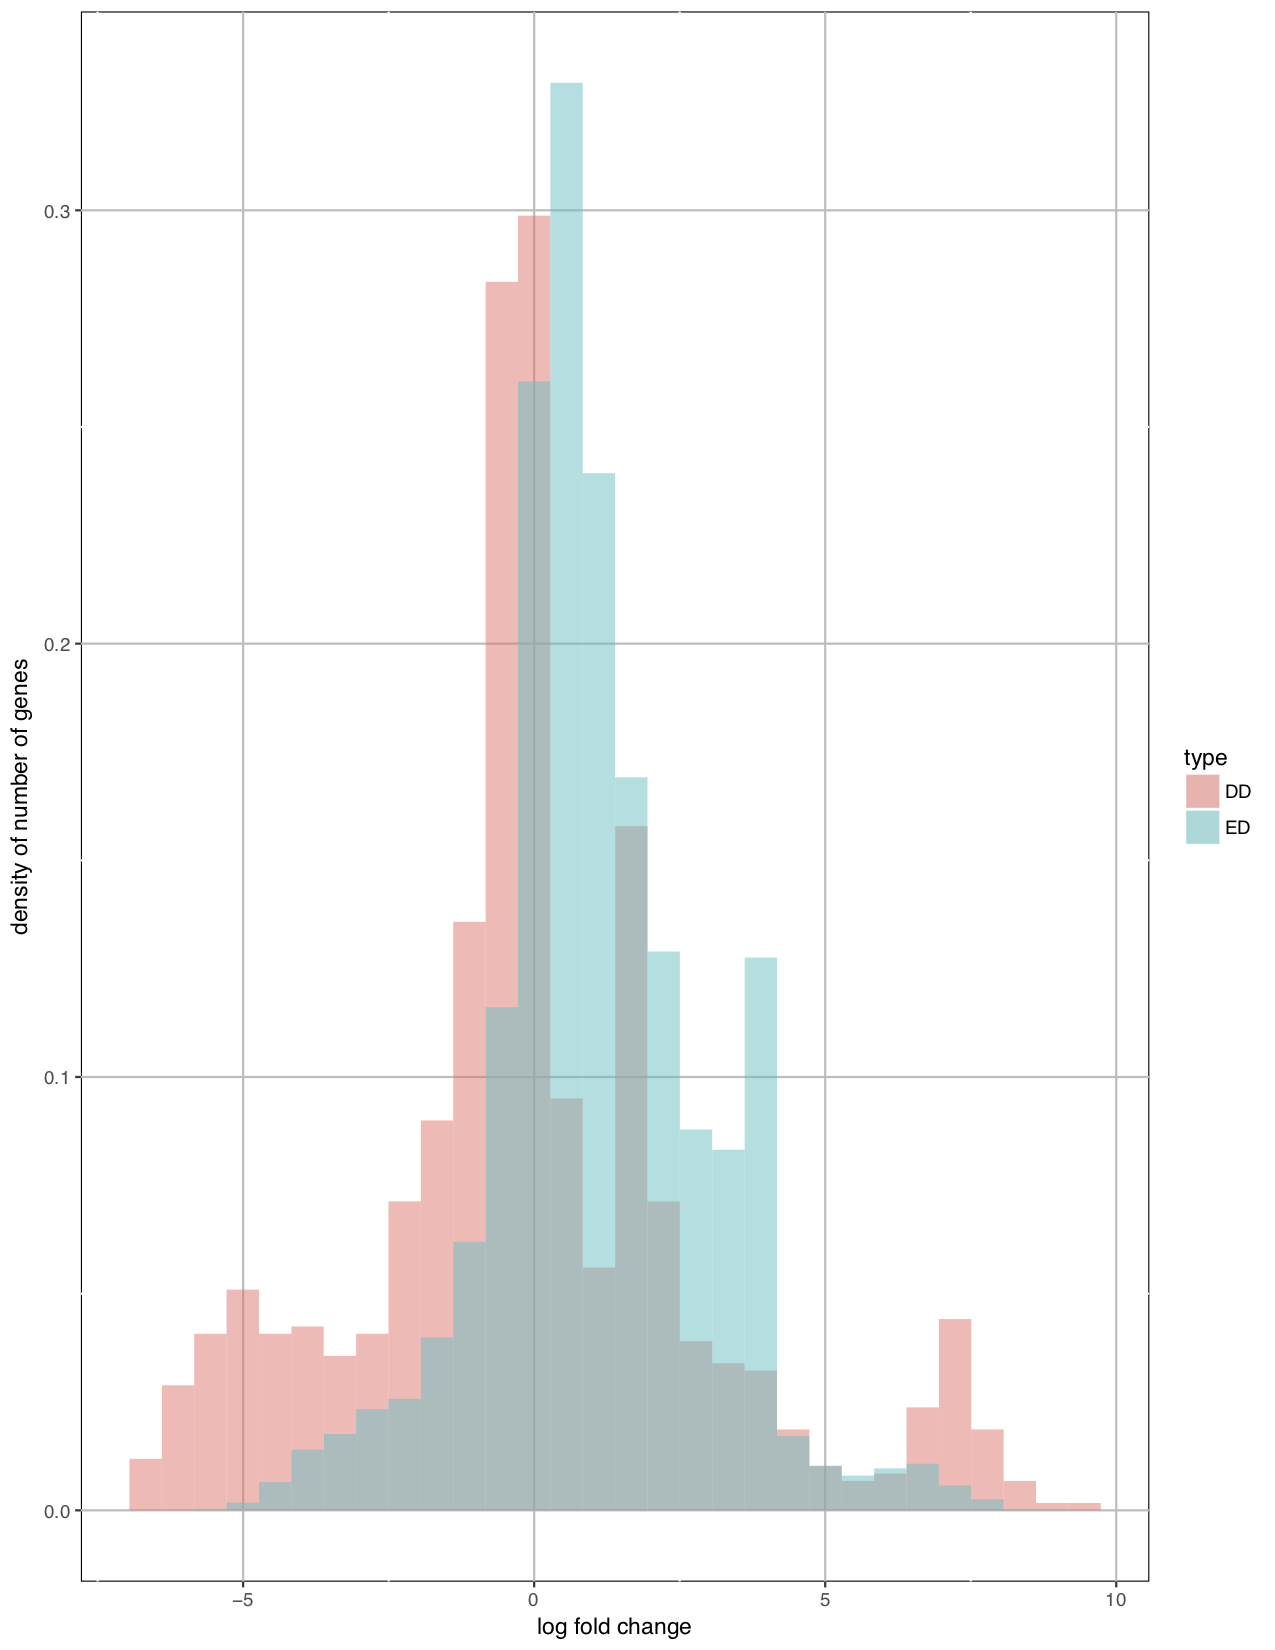
\includegraphics[width=\linewidth]{G74596_scdd.png}
  \caption{scDD}\label{fig:scDD}
\endminipage\hfill
\minipage{0.25\textwidth}
  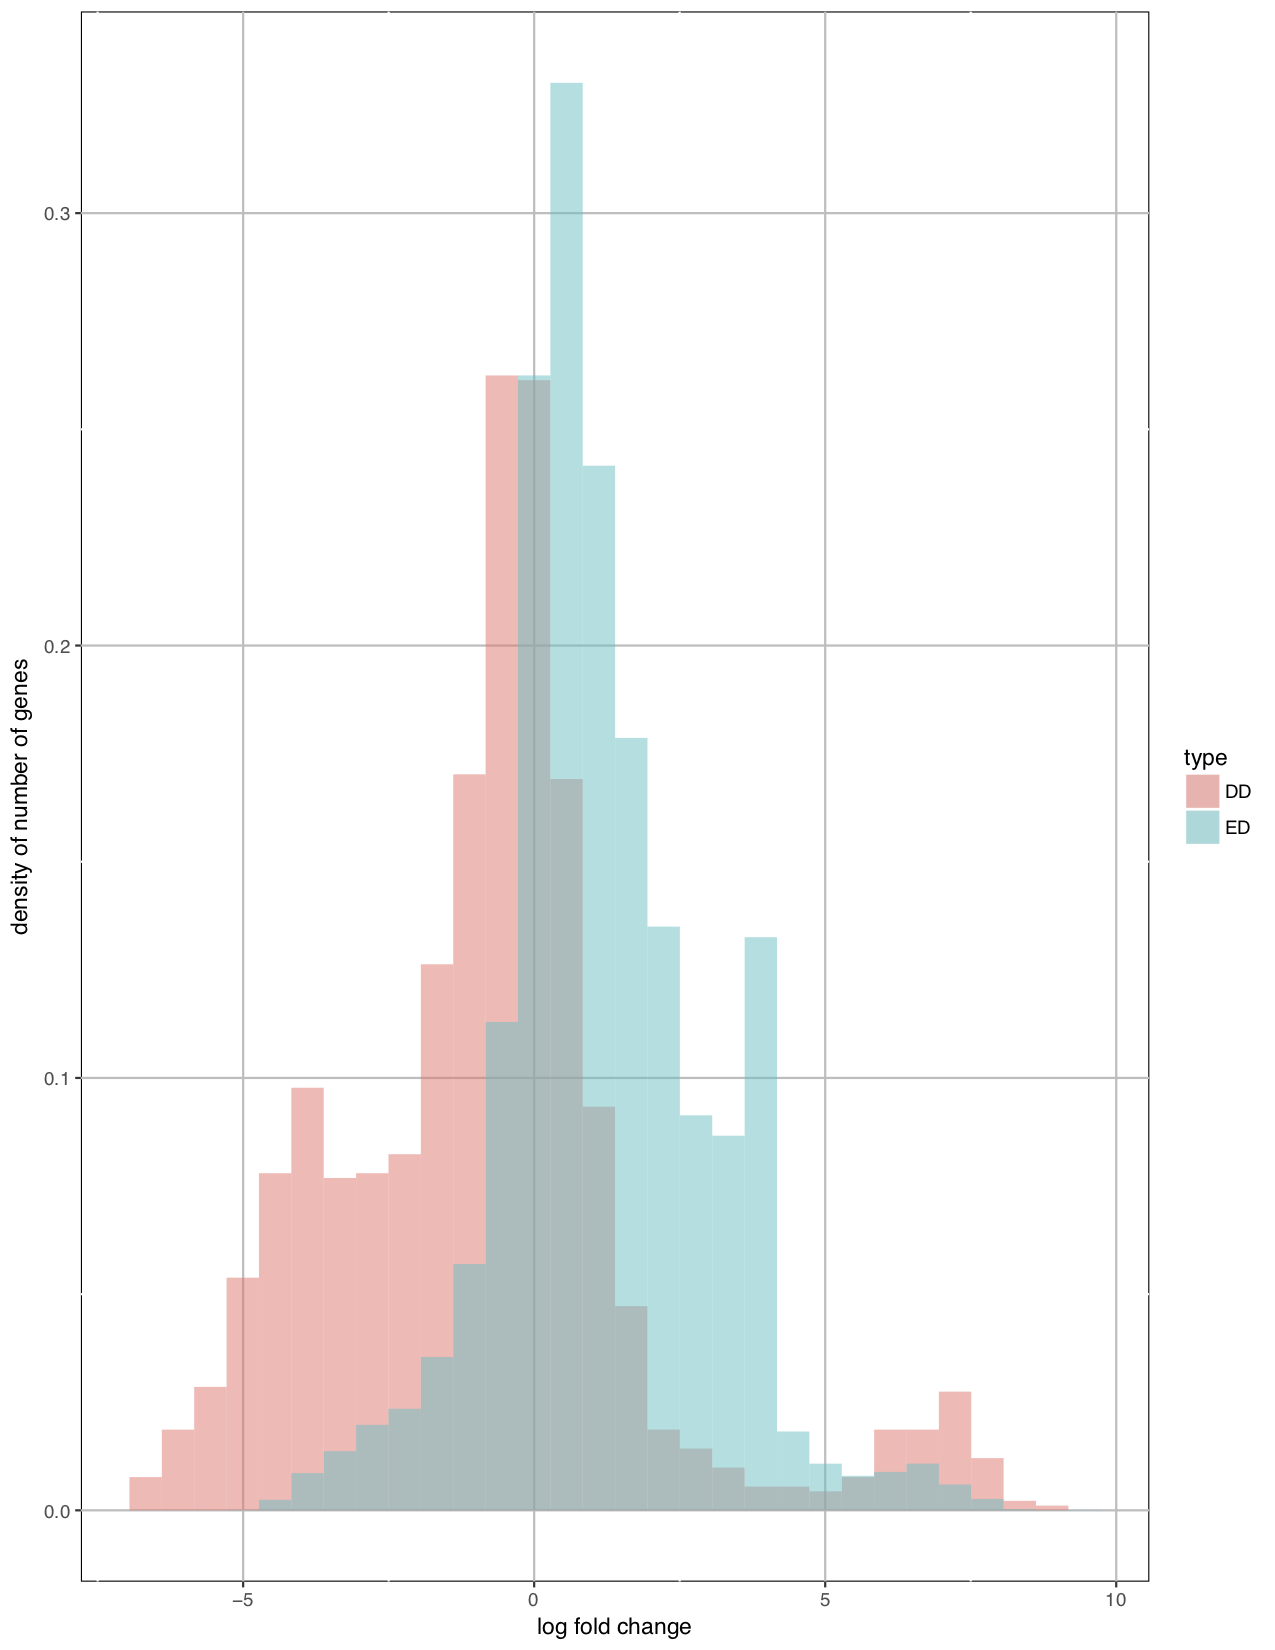
\includegraphics[width=\linewidth]{G74596_scddb.png}
  \caption{scDDboost}\label{fig:scDDboost}
\endminipage\hfill
\minipage{0.25\textwidth}%
  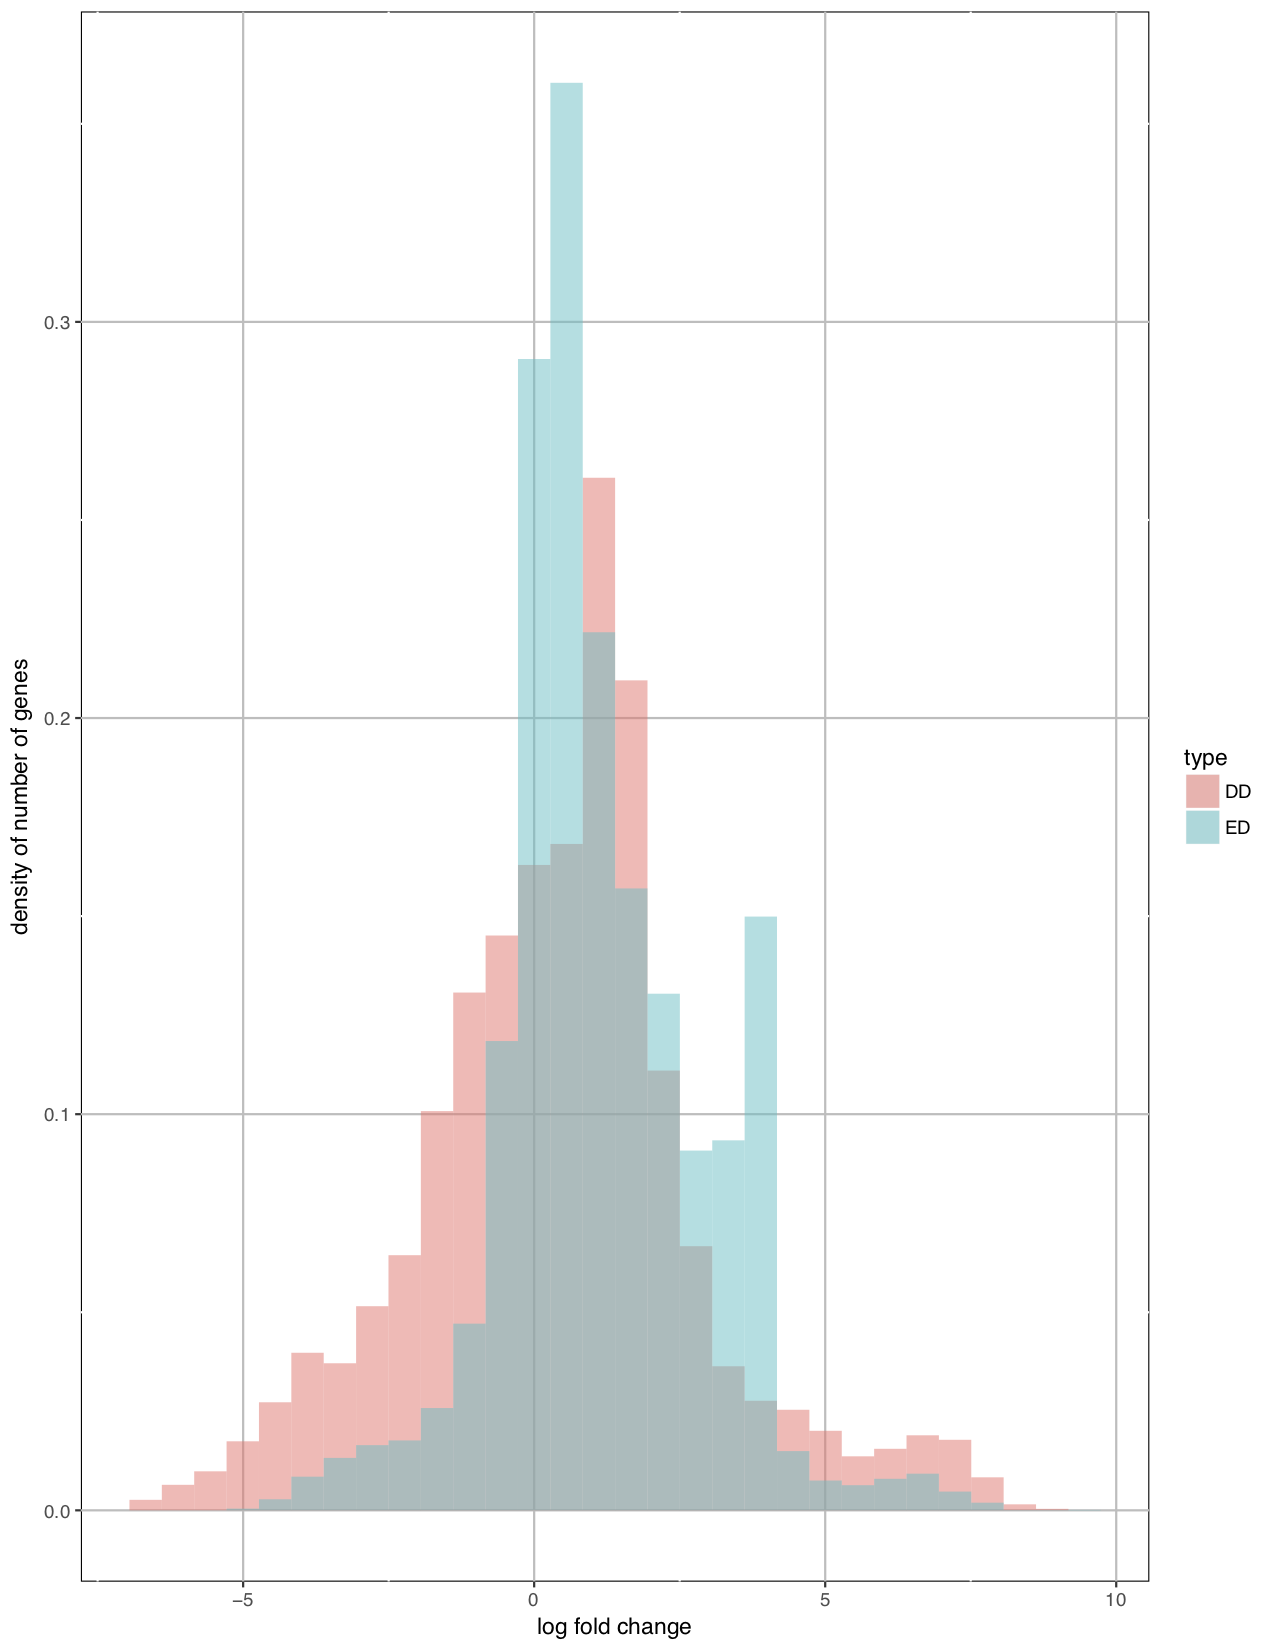
\includegraphics[width=\linewidth]{G74596_des.png}
  \caption{DESeq2}\label{fig:DESeq2}
\endminipage
\end{figure}



\cleardoublepage
\bibliographystyle{IEEEtran}
\bibliography{/Users/xiuyuma/Desktop/scDDboost_paper/scDDboost/paper/references/wlr_ref}

\end{document}  
